%%%%%%%%%%%%%%%%%%%%%%%%%%%%%%%%%%%%%%%%%%%%%%%%%%%
%% LaTeX book template                           %%
%% Author:  Amber Jain (http://amberj.devio.us/) %%
%% License: ISC license                          %%
%%%%%%%%%%%%%%%%%%%%%%%%%%%%%%%%%%%%%%%%%%%%%%%%%%%

\documentclass[a4paper,11pt]{book}
\usepackage[T1]{fontenc}
\usepackage[utf8]{inputenc}
\usepackage{lmodern}
\usepackage{listings}
\usepackage{color}
\usepackage{float}
\usepackage{tikz}
\usetikzlibrary{positioning}
\usepackage{xcolor}
\usepackage{amsmath}
\usepackage{caption}
\usetikzlibrary{matrix}
\usepackage{graphicx}
\usepackage[section]{placeins}


\newcommand*\circled[1]{\tikz[baseline=(char.base)]{
    \node[shape=circle,draw,inner sep=2pt] (char) {#1};}}

\definecolor{dkgreen}{rgb}{0,0.6,0}
\definecolor{gray}{rgb}{0.5,0.5,0.5}
\definecolor{mauve}{rgb}{0.58,0,0.82}
\lstset{frame=tb,
	language=Python,
	aboveskip=3mm,
	belowskip=3mm,
	showstringspaces=false,
	columns=flexible,
	basicstyle={\small\ttfamily},
	numbers=none,
	numberstyle=\tiny\color{gray},
	keywordstyle=\color{blue},
	commentstyle=\color{dkgreen},
	stringstyle=\color{mauve},
	breaklines=true,
	breakatwhitespace=true,
	tabsize=3
}
\usepackage{hyperref}
\usepackage{graphicx}
\usepackage[english]{babel}

%%%%%%%%%%%%%%%%%%%%%%%%%%%%%%%%%%%%%%%%%%%%%%%%%%%%%%%%%%%%%%%%%%%%%%%%%%%%%%%%
% 'dedication' environment: To add a dedication paragraph at the start of book %
% Source: http://www.tug.org/pipermail/texhax/2010-June/015184.html            %
%%%%%%%%%%%%%%%%%%%%%%%%%%%%%%%%%%%%%%%%%%%%%%%%%%%%%%%%%%%%%%%%%%%%%%%%%%%%%%%%
\newenvironment{dedication}
{
   \cleardoublepage
   \thispagestyle{empty}
   \vspace*{\stretch{1}}
   \hfill\begin{minipage}[t]{0.66\textwidth}
   \raggedright
}
{
   \end{minipage}
   \vspace*{\stretch{3}}
   \clearpage
}

%%%%%%%%%%%%%%%%%%%%%%%%%%%%%%%%%%%%%%%%%%%%%%%%
% Chapter quote at the start of chapter        %
% Source: http://tex.stackexchange.com/a/53380 %
%%%%%%%%%%%%%%%%%%%%%%%%%%%%%%%%%%%%%%%%%%%%%%%%
\makeatletter
\renewcommand{\@chapapp}{}% Not necessary...
\newenvironment{chapquote}[2][2em]
  {\setlength{\@tempdima}{#1}%
   \def\chapquote@author{#2}%
   \parshape 1 \@tempdima \dimexpr\textwidth-2\@tempdima\relax%
   \itshape}
  {\par\normalfont\hfill--\ \chapquote@author\hspace*{\@tempdima}\par\bigskip}
\makeatother

%%%%%%%%%%%%%%%%%%%%%%%%%%%%%%%%%%%%%%%%%%%%%%%%%%%
% First page of book which contains 'stuff' like: %
%  - Book title, subtitle                         %
%  - Book author name                             %
%%%%%%%%%%%%%%%%%%%%%%%%%%%%%%%%%%%%%%%%%%%%%%%%%%%

% Book's title and subtitle
\title{\Huge \textbf{Understanding Data Structures and Algorithms}
%\footnote{This is a footnote.} \\ \huge Sample book subtitle \footnote{This is yet another footnote.}
}
% Author
\author{\textsc{Using Python}
%\thanks{\url{www.example.com}}
}

\begin{document}
\frontmatter
\maketitle

\tableofcontents
\newpage

\mainmatter

%%%%%%%%%%%%%%%%
% NEW CHAPTER! %
%%%%%%%%%%%%%%%%
\chapter{Algorithmic Complexity}

\section{Complexity analysis}

The complexity of an algorithm is the amount of time and space required by an algorithm for an input of given size $n$.
\vspace{3mm}

\noindent Metric of measurement:
\begin{itemize}
    \item \textbf{Speed}: Number of operations required (best, average or worst case)
    \item \textbf{Space} Amount of memory usage
\end{itemize}

\noindent To assess the complexity, the order of the count of operation is always considered instead of the exact number of operations. We use asymptotic notation to analyze the running time of an algorithm.

\section{Asymptotic notation}

Suppose,\\
$n = $ The size of input, and \\
$f(n) = $ Number of steps to be executed by the algorithm for input size $n$

\subsubsection{$\Theta$-notation}
% $\Theta\left(g(n)\right) = \{f(n): \exists \text{ positive constant } c_1, c_2 \text{ and } n_0 \text{ such that } 0 \leq c_1g(n) \leq f(n) \leq c_2g(n), \forall n \geq n_0\}$

A function $f(n)$ belongs to set $\Theta\left(g(n)\right)$, if there exist positive constants $c_1$, $c_2$ and $n_0$ such that $c_1g(n) \leq f(n) \leq c_2g(n)$ for sufficiently large $n (n \geq n_0)$.

\subsubsection{$O$-notation (or, Big-$O$-notation)}
A function $f(n)$ belongs to set $O\left(g(n)\right)$, if there exist positive constants $c$ and $n$ such that $0 \leq f(n) \leq c_g(n)$ for $n \geq n_0$. $O$-notation provides an asymptotic upper bound.

\subsubsection{$\Omega$-notation}
A function $f(n)$ belongs to set $\Omega\left(g(n)\right)$, if there exist positive constants $c$ and $n$ such that $0 \leq c_g(n) \leq f(n)$ for $n \geq n_0$. $\Omega$-notation provides an asymptotic lower bound.

\begin{figure}[ht]
	\centering
	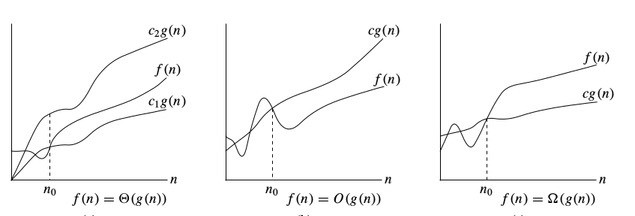
\includegraphics[scale=0.5]{pic/time.jpg}
\end{figure}

\noindent Usually we care most about upper bound on the running time of an algorithm, which is why we most often use the Big-$O$ notation for algorithm analysis.

\begin{table}[ht]
\centering
\begin{tabular}{lr}
\textbf{Time complexity}        & \textbf{Big-$O$ notation}    \\
Constant complexity    & $O(1)$              \\
Logarithmic complexity & $O(\text{log } n)$   \\
Linear complexity      & $O(n)$              \\
Quasilinear complexity & $O(n \text{log } n)$ \\
Quadratic complexity   & $O(n^2)$            \\
Qubic complexity       & $O(n^3)$            \\
Exponential complexity & $O(2^n)$            \\
Factorial complexity   & $O(n!)$            
\end{tabular}
\end{table}

\section{Recursive algorithms}

\noindent Iterative algorithms are easy to analyze which involves counting the number of elementary operations. On the other hand analyzing a recursive algorithm is a difficult task. To analyze a recursive algorithm we need to formulate a \textit{recurrence equation} (a.k.a. \textit{difference equation}). For example for the following script to generate the Fibonacci sequence, the recurrence equation for the number of operation is 
\[
   T(n) = 
\begin{cases}
    T(n-1) + T(n-2) + 4, & \text{if } n\geq 1\\
    1,              & \text{otherwise}
\end{cases}
\]

\noindent Here the constant 4 is coming due to one comparison, one addition and two subtraction operations.
\begin{lstlisting}
def fib(n):
    if (n <= 1):
        return n
    else:
        return fib(n-1) + fib(n-2)
\end{lstlisting}

\noindent We can use the substitution method to solve a recurrence equation. Substitution method involves two steps, which can be informally written as follows:
\begin{itemize}
    \item \textbf{Plug}: Substitute repeatedly
    \item \textbf{Chug}: Simplify the expression
\end{itemize}
\noindent \textbf{Example 1:} Use the substitution method for the following recurrence equation:
\[
   T(n) = 
\begin{cases}
    T(n-1) + 3, & \text{if }  n > 1\\
    4,          & \text{if }  n = 1
\end{cases}
\]

\begin{align*}
	T(n) &= T(n-1) + 3 \text{   (Plug)}\\
	     &= \left[T(n-2) + 3\right] + 3 = T(n-2) + 2\times 3 \text{   (Chug)}\\
	     &= T(n-3) + 3\times 3\\
	     &= \cdots\\
	     &= T(n-k) + k \times 3
\end{align*}
Now let's find the value of $k$ for which $n-k = 1$ i.e. $k=n-1$. Therefore,
\begin{align*}
	T(n) &= T(n-(n-1)) + (n-1)\times 3\\
	     &= T(1) + 3(n-1)\\
	     &= 4 + 3(n-1) \\
	     &= 3n + 1 \in O(n)
\end{align*}

\noindent \textbf{Example 1:} Use the substitution method for the following recurrence equation:
\[
   T(n) = 
\begin{cases}
    T(n-3) + 5, & \text{if }  n \geq 3\\
    4,          & \text{if }  n = 0, 1, 2
\end{cases}
\]

\begin{align*}
	T(n) &= T(n-3) + 5 \text{   (Plug)}\\
	     &= \left[T(n-3-3) + 5\right] + 5 = T(n-2 \times 3) + 2\times 5 \text{   (Chug)}\\
	     &= T(n-3 \times 3) + 3\times 5\\
	     &= \cdots\\
	     &= T(n-k \times 3) + k \times 5
\end{align*}
Now let's find the value of $k$ for which $n-3k = 0$ i.e. $k=\dfrac{n}{3}$. If $k$ is integer, we can write
\begin{align*}
	T(n) &= T(0) + \dfrac{n}{3}\times 5\\
	     &= 4 + \dfrac{5n}{3} \in O(n)
\end{align*}

\noindent If $\dfrac{n}{3}$ is not an integer, then find the value of integer $k = \lfloor \frac{n}{3} \rfloor$ so that,

$$n = 3\times\lfloor \frac{5n}{3} \rfloor + n\%3 $$

\noindent Putting the value of $k= \lfloor \frac{n}{3} \rfloor$ in the expression of $T(n)$
\begin{align*}
	T(n) &= T\left(n - 3\times\lfloor \frac{5n}{3} \rfloor\right) + \lfloor \frac{5n}{3} \rfloor \times 5\\
	     &= T(n\%3) + \lfloor \frac{5n}{3} \rfloor \times 5\\
	     &= 4 + \lfloor \frac{5n}{3} \rfloor \times 5 \in O(n)
\end{align*}

\noindent \textbf{Example 3:} Try the substitution method for the recurrence equation of the Fibonacci sequence:
\[
   T(n) = 
\begin{cases}
    T(n-1) + T(n-2) + c, & \text{if } n > 1\\
    1,                   & \text{if } n = 0, 1
\end{cases}
\]

\begin{align*}
	T(n) &= T(n-1) + T(n-2) + c \\
	     &\leq 2T(n-1) + c \\
	     &= 2\left[2T(n-2) + c\right] + c\\
	     &= 2^2T(n-2) + 2c + c\\
	     &= 2^2\left[2T(n-3) + c\right] + 2c + c\\
	     &= 2^3 T(n-3) + 2^2c + 2c + c\\
	     &= \cdots\\
	     &= 2^k T(n-k) + \underbrace{2^{k-1}c + 2^{k-2}c + \cdots + 2^2c + 2c + c}_{(2^k-1)c}\\
\end{align*}
Now let's find the value of $k$ for which $n-k = 0$ i.e. $k=n$. Therefore,
\begin{align*}
	T(n) &= 2^n T(0) + (2^n-1)\times c\\
	     &= 2^n (1+c) - c \in O(2^n)
\end{align*}

\noindent \textbf{Example 4:} Solve the recurrence equation of the form:
\[
   T(n) = 
\begin{cases}
    T(n-1) + T(n-2) + T(n-3) + c, & \text{if } n > 2\\
    1,                   & \text{if } n = 0, 1, 2
\end{cases}
\]

\noindent In the similar way as before it can be shown that the time complexity for this problem is
$$T(n) \in O(3^n)$$

\noindent \textbf{Example 5:} Solve the recurrence equation of the form (Geometric sequence):
\[
   T(n) = 
\begin{cases}
    rT(n-1) , & \text{if } n > 0\\
    \alpha,                   & \text{if } n = 0
\end{cases}
\]

\begin{align*}
	T(n) &= rT(n-1) \\
	     & r \times \left[rT(n-2)\right] = r^2 T[n-2] \\
	     &= r^2 \times \left[rT(n-3)\right] = r^3 T[n-3]\\
	     &= \cdots\\
	     &= r^k T[n-k]\\
\end{align*}
\noindent Now let's find the value of $k$ for which $n-k = 0$ i.e. $k=n$. Therefore,
\begin{align*}
	T(n) &= r^n T(0)\\
	     &= \alpha r^n \in O(r^n)
\end{align*}

\noindent \textbf{Example 6:} Solve the recurrence equation for calculating factorial:
\[
   T(n) = 
\begin{cases}
    nT(n-1) , & \text{if } n > 0\\
    0,                   & \text{if } n = 0
\end{cases}
\]

\begin{align*}
	T(n) &= nT(n-1) \\
	     & n \times \left[(n-1)T(n-2)\right] = n(n-1) T[n-2] \\
	     &= n(n-1) \times \left[(n-2)T(n-3)\right] = n(n-1)(n-2) T[n-3]\\
	     &= \cdots\\
	     &= n(n-1)(n-2) \cdots (n-(k-1)T[n-k]\\
\end{align*}
\noindent Now let's find the value of $k$ for which $n-k = 0$ i.e. $k=n$. Therefore,
\begin{align*}
	T(n) &= n(n-1)(n-2) \cdots (n-(n-1))T[0]\\
	     &= n(n-1)(n-2) \cdots 1\\
	     &= n! \in O(n!)
\end{align*}
\section{Master Theorem}

\noindent The Master theorem is a general method for solving (getting time complexity for) recurrence relations that arise frequently in \textit{divide and conquer algorithms}, which have the following recurrence relation of the form: 
$$T(n) = a T\left(\dfrac{n}{b}\right)+f(n)$$
\noindent where $a \ge 1$, $b > 1$, and $f(n)$ is an asymptotically positive function. The time complexity of such a recursive relation is given by the following rules:

\begin{enumerate}
\item If $f(n) = O(n^{\log_ba-\epsilon})$ for some constant
$\epsilon>0$, then $T(n) = \Theta(n^{\log_ba})$.
\item If $f(n) = \Theta(n^{\log_ba})$, then $T(n) =
\Theta(n^{\log_ba} \log n)$.
\item If $f(n) = \Omega(n^{\log_ba+\epsilon})$ for some constant $\epsilon>0$, and if $a f(n/b) \le c f(n)$ for some constant $c<1$ and all sufficiently large $n$, then $T(n) = \Theta(f(n))$.
\item If $f(n) = \Theta(n^{\log_ba} \log^k(n))$ for $k\ge 0$, then
$T(n) = \Theta(n^{\log_ba} \log^{k+1} n)$.
\end{enumerate}

\noindent Simply put, if $f(n)$ is polynomially smaller than $n^{\log_b{a}}$, then the runtime is $\Theta(n^{\log_ba})$. If $f(n)$ is instead polynomially larger than $n^{\log_b{a}}$, then the runtime is $\Theta(f(n)$. Finally, if $f(n)$ and $n^{\log_b{a}}$ are asymptotically the same, then the runtime is  $\Theta(n^{\log_ba} \log n)$.
\vspace{3mm}

\noindent \textbf{Example 1.} $T(n) = 9 T(n/3) + n$

\begin{itemize} 
\item Here $a = 9$, $b=3$, $f(n) = n$, $n^{\log_ba} = n^2$.  $n^2$ is
polynomially bigger.
\item So, $T(n) = \Theta(n^{\log_ba}) = \Theta(n^2)$.
\end{itemize}

\noindent \textbf{Example 2.} $T(n) = \Theta(f(n)) = 3 T(n/7) + n^{\frac{3}{4}}$

\begin{itemize} 
\item Here $a = 3$, $b=7$, $f(n) = n^{\frac{3}{4}} = n^{0.75}$,
$n^{\log_ba} \approx n^{0.56}$.  $n^{0.75}$ is polynomially bigger.
\item So, $T(n) = \Theta(f(n)) = \Theta(n^{\frac{3}{4}})$.
\end{itemize}

\noindent Note: Since $a f(n/b) \le c f(n)$ for some constant $c<1$ and all sufficiently large $n$, Master Theorem definitely applies!
\vspace{3mm}

\noindent \textbf{Example 3.} $T(n) = T(4n/5) + \log^2 n$

\begin{itemize} 
\item Here $a = 1$, $b=5/4$, $f(n) = \log^2 n$, $n^{\log_ba} =
1$. $f(n)$ is not polynomially bigger. But Rule 4 applies (with
$k=2$).
\item So, $T(n) = \Theta(\log^3(n))$.
\end{itemize}

\noindent \textbf{Example 4.} $T(n) = 2 T(n/4) + \sqrt{n} \log \log(n)$

\begin{itemize} 
\item Here $a = 2$, $b=4$, $f(n) = \sqrt{n}\log\log n$, $n^{\log_ba}
=n^{1/2}$, so $f(n)$ is not polynomially larger than  $n^{\log_ba}$, it is larger only by a logarithmic factor.
\item So, Master Theorem does not apply.
\end{itemize}

\chapter{Data Structures}

\section{Linked list}

A linked list is a linear collection of data elements in which the linear ordering is maintained by each element pointing to the next (not by physical placements in memory). It is a data structure consisting of a group of nodes which together form a sequence. Each node is composed of two parts: \textbf{data} and a \textbf{reference} (link) to the next node in the sequence.\\

\textbf{Advantages:}
\begin{enumerate}
	\item Unlike list (array), they are dynamic in nature which allocates memory whenever required.
	\item This structure allows efficient insertion and removal of elements.
	\item Stacks and queues can easily be implemented.
	\item Linked list reduces the access time.
\end{enumerate}

\textbf{Disadvantages:}
\begin{enumerate}
	\item The memory is wasted as the reference requires extra memory for storage.
	\item No element can be accessed randomly.
	\item Reverse traversing is difficult.
\end{enumerate}

\subsection{Inserting item into linked list}
\begin{lstlisting}
class Node:
    # Constructor
    def __init__(self, data):
        self.data = data
        self.next = None

class LinkedList:
    # Constructor
    def __init__(self):
        self.head = None

    # Display the linked list
    def display(self):
        cur_node = self.head
        while cur_node:
            print('['+str(cur_node.data)+'] ---> ', end='')
            cur_node = cur_node.next
        print('None')

    # Returns the length of the linked list
    def length(self):
        count = 0
        cur_node = self.head

        while cur_node:
            count += 1
            cur_node = cur_node.next
        return count

    # Insert item at the end of linked list
    # Time complexity: O(n)
    def insertLast(self, data):
        new_node = Node(data)

        if self.head is None:
            self.head = new_node
            return None

        last_node = self.head
        while last_node.next:
            last_node = last_node.next
        last_node.next = new_node

    # Insert item at the beginning of linked list
    # Time complexity: O(1)
    def insertFirst(self, data):
        new_node = Node(data)

        new_node.next = self.head
        self.head = new_node

    # Insert item at a specific position of linked list
    def insert_at_pos(self, pos, data):
        if pos < 0 or pos > self.length():
            print('No node exists at this position')
            return None
        
        new_node = Node(data)
        cur_node = self.head
        if pos == 0:
            self.insertFirst(data)
        else:
            for _ in range(pos-1):
                cur_node = cur_node.next
            new_node.next = cur_node.next
            cur_node.next = new_node

if __name__ == "__main__":
    linklist_obj = LinkedList()
    linklist_obj.insertLast("B")
    linklist_obj.insertLast("C")
    linklist_obj.insertFirst("A")
    linklist_obj.display()

    linklist_obj.insert_at_pos(2, 'D')
    linklist_obj.insert_at_pos(1, 5)
    linklist_obj.display()
\end{lstlisting}
\textbf{Output}
\begin{lstlisting}
[A] ---> [B] ---> [C] ---> None
[A] ---> [5] ---> [B] ---> [D] ---> [C] ---> None
\end{lstlisting}

\subsection{Deleting item from linked list}
\vspace{5mm}

To delete a node from the linked list, we need to do the following steps.
\begin{itemize}
    \item Find the previous node of the node to be deleted.
    \item Make the previous node point to the node which is after the node to be deleted.
    \item Free memory for the node to be deleted.
\end{itemize}

\begin{center}
    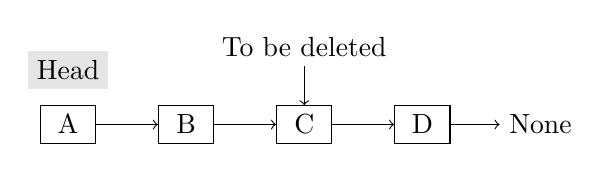
\begin{tikzpicture}[
    every node/.style = {minimum width = 2em, draw, rectangle, node distance={15mm}},
      level/.style = {sibling distance = 30mm/#1}
    ]
    \node (1) {A};
    \node[draw=none, fill=gray!20] (1a) [above=.2cm of 1] {Head};
    \node (2) [right of=1] {B};
    \node (3) [right of=2] {C}; 
    \node[draw=none] (3a) [above=.5cm of 3] {To be deleted};
    \node (4) [right of=3] {D};
    \node[draw=none] (5) [right of=4] {None};
    \draw[->] (1) -- (2);
    \draw[->] (2) -- (3);
    \draw[->] (3a) -- (3);
    \draw[->] (3) -- (4);
    \draw[->] (4) -- (5);
    \end{tikzpicture}
\end{center}

\begin{center}
    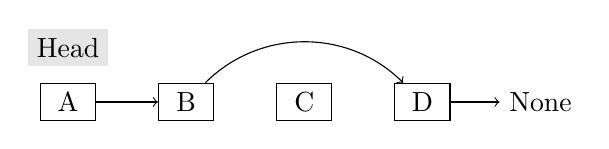
\begin{tikzpicture}[>=to, 
    every node/.style = {minimum width = 2em, draw, rectangle, node distance={15mm}},
      level/.style = {sibling distance = 30mm/#1}
    ]
    \node (1) {A};
    \node[draw=none, fill=gray!20] (1a) [above=.2cm of 1] {Head};
    \node (2) [right of=1] {B};
    \node (3) [right of=2] {C};
    \node (4) [right of=3] {D};
    
    \node[draw=none] (5) [right of=4] {None};
    \draw[->] (1) -- (2);
    \draw[->] (2) to[out=45, in=135] (4);
    \draw[->] (4) -- (5);
    \end{tikzpicture}
\end{center}

\begin{center}
    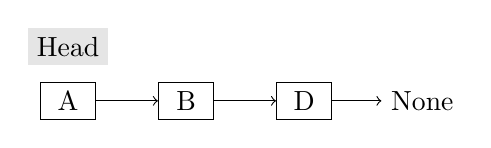
\begin{tikzpicture}[>=to, 
    every node/.style = {minimum width = 2em, draw, rectangle, node distance={15mm}},
      level/.style = {sibling distance = 30mm/#1}
    ]
    \node (1) {A};
    \node[draw=none, fill=gray!20] (1a) [above=.2cm of 1] {Head};
    \node (2) [right of=1] {B};
    \node (4) [right of=2] {D};
    
    \node[draw=none] (5) [right of=4] {None};
    \draw[->] (1) -- (2);
    \draw[->] (2) -- (4);
    \draw[->] (4) -- (5);
    \end{tikzpicture}
\end{center}

\noindent Time complexity: $O(n)$

\begin{lstlisting}
# Delete item by value (key)
def delete_by_key(self, key):

    cur_node = self.head

    if cur_node and cur_node.data == key:
        self.head = cur_node.next
        cur_node = None
        return None

    prev_node = None 
    while cur_node and cur_node.data != key:
        prev_node = cur_node
        cur_node = cur_node.next

    if cur_node is None:
        return None

    prev_node.next = cur_node.next
    cur_node = None

# Delete item by position(index)
def delete_at_pos(self, pos):

    cur_node = self.head

    if pos == 0:
        self.head = cur_node.next
        cur_node = None
        return None

    prev_node = None
    count = 1
    while cur_node and count != pos:
        prev_node = cur_node 
        cur_node = cur_node.next
        count += 1

    if cur_node is None:
        return 

    prev_node.next = cur_node.next
    cur_node = None
\end{lstlisting}

\subsection{Search element in a linked list using key}
\vspace{5mm}

\noindent Time complexity: $O(n)$

\begin{lstlisting}
# Search element in a linked list using key
def searchkey(self, key):
    cur_node = self.head
    pos = 0
    
    if self.head == None:
        print('No such value found in the Linked List')
    else:
        while cur_node:
            if cur_node.data == key:
                print("Search value index = "+str(pos))
                return None
            cur_node = cur_node.next
            pos += 1
        if cur_node == None:
            print('No such value found in the Linked List')
\end{lstlisting}

\subsection{Reversing a linked list}
\vspace{5mm}

\noindent Iterative method:

\begin{enumerate}
    \item Initialize pointers \lstinline{prev_node} as NULL, \lstinline{cur_node} as \lstinline{head}.
    \item Iterate through the linked list. In loop, do following.
    \begin{enumerate}
        \item Create a \lstinline{next_node} pointer for saving \lstinline{current_node.next}
        \item Point the \lstinline{cur_node} point to the previous node.
        \item Move \lstinline{prev_node} and \lstinline{cur_node} one step forward 
    \end{enumerate}
\end{enumerate}

\begin{center}
    \begin{tikzpicture}[>=to, 
    every node/.style = {minimum width = 2em, draw, rectangle, node distance={23mm}},
      level/.style = {sibling distance = 30mm/#1}
    ]
    \node[draw=none] (0) [left of=1] {None};
    \node[draw=none, fill=gray!20] (0a) [below=.4cm of 0] {\lstinline{prev_node}};
    \node (1) {A};
    \node[draw=none, fill=gray!20] (1a) [below=.4cm of 1] {\lstinline{cur_node}};
    \node (2) [right of=1] {B};
    \node[draw=none, fill=gray!20] (2a) [below=.4cm of 2] {\lstinline{next_node}};
    \node (3) [right of=2] {C};
    
    \node[draw=none] (4) [right of=3] {None};
    \draw[->] (1) -- (2);
    \draw[->] (2) -- (3);
    \draw[->] (3) -- (4);
    \end{tikzpicture}
\end{center}

\begin{center}
    \begin{tikzpicture}[>=to, 
    every node/.style = {minimum width = 2em, draw, rectangle, node distance={23mm}},
      level/.style = {sibling distance = 30mm/#1}
    ]
    \node[draw=none] (0) [left of=1] {None};
    \node[draw=none, fill=gray!20] (0a) [below=.4cm of 0] {\lstinline{prev_node}};
    \node (1) {A};
    \node[draw=none, fill=gray!20] (1a) [below=.4cm of 1] {\lstinline{cur_node}};
    \node (2) [right of=1] {B};
    \node[draw=none, fill=gray!20] (2a) [below=.4cm of 2] {\lstinline{next_node}};
    \node (3) [right of=2] {C};
    
    \node[draw=none] (4) [right of=3] {None};
    \draw[->] (1) -- (0);
    \draw[->] (2) -- (3);
    \draw[->] (3) -- (4);
    \end{tikzpicture}
\end{center}

\begin{center}
    \begin{tikzpicture}[>=to, 
    every node/.style = {minimum width = 2em, draw, rectangle, node distance={23mm}},
      level/.style = {sibling distance = 30mm/#1}
    ]
    \node[draw=none] (0) [left of=1] {None};
    \node[draw=none, fill=gray!20] (0a) [below=.4cm of 1] {\lstinline{prev_node}};
    \node (1) {A};
    \node[draw=none, fill=gray!20] (1a) [below=.4cm of 2] {\lstinline{cur_node}};
    \node (2) [right of=1] {B};
    \node[draw=none, fill=gray!20] (2a) [below=.4cm of 3] {\lstinline{next_node}};
    \node (3) [right of=2] {C};
    
    \node[draw=none] (4) [right of=3] {None};
    \draw[->] (1) -- (0);
    \draw[->] (2) -- (3);
    \draw[->] (3) -- (4);
    \end{tikzpicture}
\end{center}

\begin{center}
    \begin{tikzpicture}[>=to, 
    every node/.style = {minimum width = 2em, draw, rectangle, node distance={23mm}},
      level/.style = {sibling distance = 30mm/#1}
    ]
    \node[draw=none] (0) [left of=1] {None};
    \node[draw=none, fill=gray!20] (0a) [below=.4cm of 1] {\lstinline{prev_node}};
    \node (1) {A};
    \node[draw=none, fill=gray!20] (1a) [below=.4cm of 2] {\lstinline{cur_node}};
    \node (2) [right of=1] {B};
    \node[draw=none, fill=gray!20] (2a) [below=.4cm of 3] {\lstinline{next_node}};
    \node (3) [right of=2] {C};
    
    \node[draw=none] (4) [right of=3] {None};
    \draw[->] (1) -- (0);
    \draw[->] (2) -- (1);
    \draw[->] (3) -- (4);
    \end{tikzpicture}
\end{center}

\begin{center}
    \begin{tikzpicture}[>=to, 
    every node/.style = {minimum width = 2em, draw, rectangle, node distance={23mm}},
      level/.style = {sibling distance = 30mm/#1}
    ]
    \node[draw=none] (0) [left of=1] {None};
    \node[draw=none, fill=gray!20] (0a) [below=.4cm of 2] {\lstinline{prev_node}};
    \node (1) {A};
    \node[draw=none, fill=gray!20] (1a) [below=.4cm of 3] {\lstinline{cur_node}};
    \node (2) [right of=1] {B};
    \node[draw=none, fill=gray!20] (2a) [below=.4cm of 4] {\lstinline{next_node}};
    \node (3) [right of=2] {C};
    
    \node[draw=none] (4) [right of=3] {None};
    \draw[->] (1) -- (0);
    \draw[->] (2) -- (1);
    \draw[->] (3) -- (4);
    \end{tikzpicture}
\end{center}

\begin{center}
    \begin{tikzpicture}[>=to, 
    every node/.style = {minimum width = 2em, draw, rectangle, node distance={23mm}},
      level/.style = {sibling distance = 30mm/#1}
    ]
    \node[draw=none] (0) [left of=1] {None};
    \node[draw=none, fill=gray!20] (0a) [below=.4cm of 2] {\lstinline{prev_node}};
    \node (1) {A};
    \node[draw=none, fill=gray!20] (1a) [below=.4cm of 3] {\lstinline{cur_node}};
    \node (2) [right of=1] {B};
    \node (3) [right of=2] {C};
    
    \draw[->] (1) -- (0);
    \draw[->] (2) -- (1);
    \draw[->] (3) -- (2);
    \end{tikzpicture}
\end{center}

\noindent Time complexity: $O(n)$\\
\noindent Space complexity: $O(1)$

\begin{lstlisting}
 def reverse(self):
    cur_node = self.head
    prev_node = None
    
    while cur_node:
        next_node = cur_node.next
        # next_node for saving cur_node.next
        cur_node.next = prev_node
        prev_node = cur_node
        cur_node = next_node
    self.head = prev_node
\end{lstlisting}

\noindent Using recursive method:

\begin{enumerate}
    \item Divide the list in two parts - first node and 
      rest of the linked list.
   \item Call reverse for the rest of the linked list.
   \item Link rest to first.
   \item Fix head pointer
\end{enumerate}

\begin{center}
    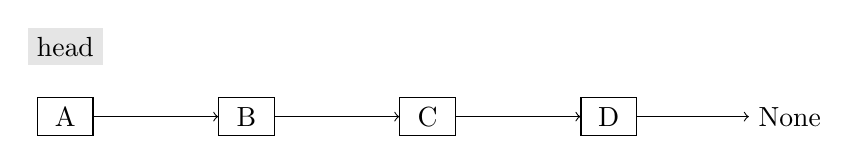
\begin{tikzpicture}[>=to, 
    every node/.style = {minimum width = 2em, draw, rectangle, node distance={23mm}},
      level/.style = {sibling distance = 30mm/#1}
    ]
    \node (A) {A};
    \node[draw=none, fill=gray!20] (A1) [above=.4cm of A] {\lstinline{head}};
    \node (B) [right of=A] {B};
    \node (C) [right of=B] {C};
    \node (D) [right of=C] {D};
    \node[draw=none] (E) [right of=D] {None};
    
    \draw[->] (A) -- (B);
    \draw[->] (B) -- (C);
    \draw[->] (C) -- (D);
    \draw[->] (D) -- (E);
    \end{tikzpicture}
\end{center}

\begin{center}
    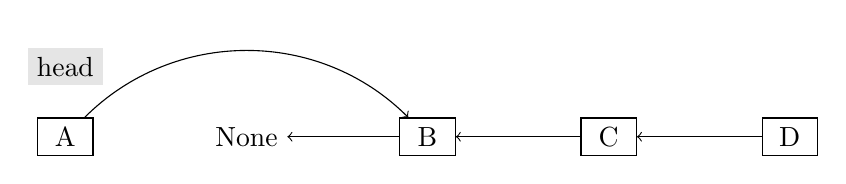
\begin{tikzpicture}[>=to, 
    every node/.style = {minimum width = 2em, draw, rectangle, node distance={23mm}},
      level/.style = {sibling distance = 30mm/#1}
    ]
    \node (A) {A};
    \node[draw=none, fill=gray!20] (A1) [above=.4cm of A] {\lstinline{head}};
    \node[draw=none] (E) [right of=A] {None};
    \node (B) [right of=E] {B};
    \node (C) [right of=B] {C};
    \node (D) [right of=C] {D};
    
    \draw[->] (A) to[out=45, in=135] (B);
    \draw[->] (D) -- (C);
    \draw[->] (C) -- (B);
    \draw[->] (B) -- (E);
    \end{tikzpicture}
\end{center}
\vspace{5mm}
\begin{center}
    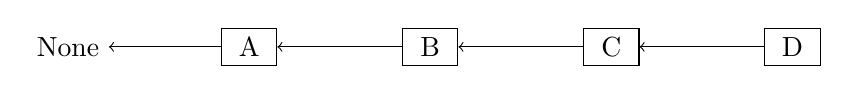
\begin{tikzpicture}[>=to, 
    every node/.style = {minimum width = 2em, draw, rectangle, node distance={23mm}},
      level/.style = {sibling distance = 30mm/#1}
    ]
    \node (A) {A};
    \node[draw=none] (E) [left of=A] {None};
    \node (B) [right of=A] {B};
    \node (C) [right of=B] {C};
    \node (D) [right of=C] {D};
    
    \draw[->] (A) -- (E);
    \draw[->] (B) -- (A);
    \draw[->] (D) -- (C);
    \draw[->] (C) -- (B);
    \end{tikzpicture}
\end{center}

\noindent Time complexity: $O(n)$\\
\noindent Space complexity: $O(1)$

\begin{lstlisting}
def reverse(self, head):
    # If head is empty or has reached the list end
    if head is None or head.next is None:
        return head

    # Reverse the rest list
    rest = self.reverse(head.next)

    # Put first element at the end
    head.next.next = head
    
    # Fix the header pointer
    head.next = None
    
    return rest
\end{lstlisting}

\subsection{Check if a linked list is palindrome or not (in constant space complexity)}
\vspace{5mm}

\begin{enumerate}
    \item Divide the list into two equal parts. If the linked list contains an odd number of nodes, then ignore the middle element.
    \begin{enumerate}
        \item Create two pointers \lstinline{slow} and \lstinline{fast} which moves by one node and two nodes at a time respectively. Both start at the head.
        \item After traversing the list, the \lstinline{fast} pointer would point to the last node if the number of nodes is odd. If the number of nodes is even, the \lstinline{fast} pointer would point to the None.
        \begin{figure}
        \begin{center}
        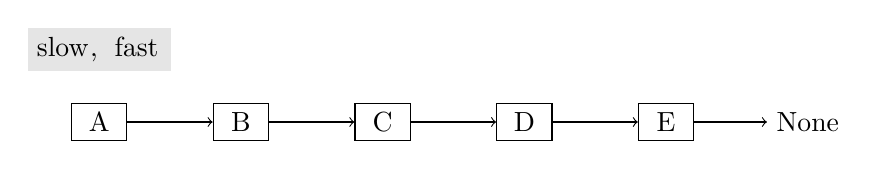
\begin{tikzpicture}[>=to, 
        every node/.style = {minimum width = 2em, draw, rectangle, node distance={18mm}},
          level/.style = {sibling distance = 30mm/#1}
        ]
        \node (A) {A};
        \node[draw=none, fill=gray!20] (A1) [above=.4cm of A] {\lstinline{slow, fast}};
        \node (B) [right of=A] {B};
        \node (C) [right of=B] {C};
        \node (D) [right of=C] {D};
        \node (E) [right of=D] {E};
        \node[draw=none] (F) [right of=E] {None};
        
        \draw[->] (A) -- (B);
        \draw[->] (B) -- (C);
        \draw[->] (C) -- (D);
        \draw[->] (D) -- (E);
        \draw[->] (E) -- (F);
        \end{tikzpicture}
        \end{center}
        \begin{center}
        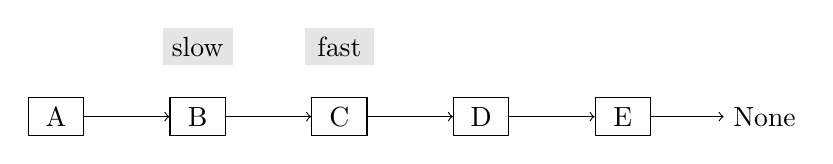
\begin{tikzpicture}[>=to, 
        every node/.style = {minimum width = 2em, draw, rectangle, node distance={18mm}},
          level/.style = {sibling distance = 30mm/#1}
        ]
        \node (A) {A};
        \node (B) [right of=A] {B};
        \node[draw=none, fill=gray!20] (B1) [above=.4cm of B] {\lstinline{slow}};
        \node (C) [right of=B] {C};
        \node[draw=none, fill=gray!20] (C1) [above=.4cm of C] {\lstinline{fast}};
        \node (D) [right of=C] {D};
        \node (E) [right of=D] {E};
        \node[draw=none] (F) [right of=E] {None};
        
        \draw[->] (A) -- (B);
        \draw[->] (B) -- (C);
        \draw[->] (C) -- (D);
        \draw[->] (D) -- (E);
        \draw[->] (E) -- (F);
        \end{tikzpicture}
        \end{center}
        \begin{center}
        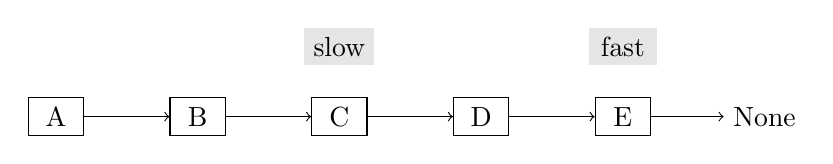
\begin{tikzpicture}[>=to, 
        every node/.style = {minimum width = 2em, draw, rectangle, node distance={18mm}},
          level/.style = {sibling distance = 30mm/#1}
        ]
        \node (A) {A};
        \node (B) [right of=A] {B};
        \node (C) [right of=B] {C};
        \node (D) [right of=C] {D};
        \node[draw=none, fill=gray!20] (C1) [above=.4cm of C] {\lstinline{slow}};
        \node (E) [right of=D] {E};
        \node[draw=none, fill=gray!20] (E1) [above=.4cm of E] {\lstinline{fast}};
        \node[draw=none] (F) [right of=E] {None};
        
        \draw[->] (A) -- (B);
        \draw[->] (B) -- (C);
        \draw[->] (C) -- (D);
        \draw[->] (D) -- (E);
        \draw[->] (E) -- (F);
        \end{tikzpicture}
        \end{center}
        \captionsetup{labelformat=empty}
        \caption{Movement of \lstinline{slow} and \lstinline{fast} pointers for odd number of nodes} 
        \label{fig:Odd}
        \end{figure}
        	
	\begin{figure}
	\begin{center}
        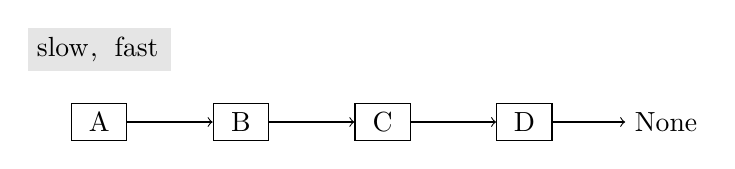
\begin{tikzpicture}[>=to, 
        every node/.style = {minimum width = 2em, draw, rectangle, node distance={18mm}},
          level/.style = {sibling distance = 30mm/#1}
        ]
        \node (A) {A};
        \node[draw=none, fill=gray!20] (A1) [above=.4cm of A] {\lstinline{slow, fast}};
        \node (B) [right of=A] {B};
        \node (C) [right of=B] {C};
        \node (D) [right of=C] {D};
        \node[draw=none] (E) [right of=D] {None};
        
        \draw[->] (A) -- (B);
        \draw[->] (B) -- (C);
        \draw[->] (C) -- (D);
        \draw[->] (D) -- (E);
        \end{tikzpicture}
        \end{center}
        \begin{center}
        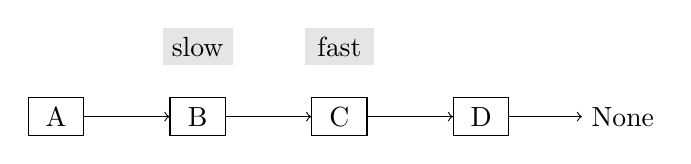
\begin{tikzpicture}[>=to, 
        every node/.style = {minimum width = 2em, draw, rectangle, node distance={18mm}},
          level/.style = {sibling distance = 30mm/#1}
        ]
        \node (A) {A};
        \node (B) [right of=A] {B};
        \node[draw=none, fill=gray!20] (B1) [above=.4cm of B] {\lstinline{slow}};
        \node (C) [right of=B] {C};
        \node[draw=none, fill=gray!20] (C1) [above=.4cm of C] {\lstinline{fast}};
        \node (D) [right of=C] {D};
        \node[draw=none] (E) [right of=D] {None};
        
        \draw[->] (A) -- (B);
        \draw[->] (B) -- (C);
        \draw[->] (C) -- (D);
        \draw[->] (D) -- (E);
        \end{tikzpicture}
        \end{center}
        \begin{center}
        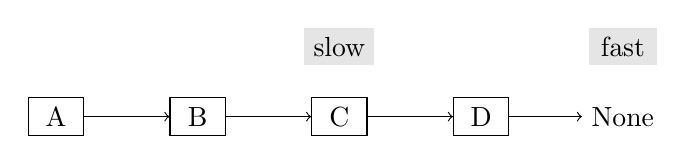
\begin{tikzpicture}[>=to, 
        every node/.style = {minimum width = 2em, draw, rectangle, node distance={18mm}},
          level/.style = {sibling distance = 30mm/#1}
        ]
        \node (A) {A};
        \node (B) [right of=A] {B};
        \node (C) [right of=B] {C};
        \node (D) [right of=C] {D};
        \node[draw=none, fill=gray!20] (C1) [above=.4cm of C] {\lstinline{slow}};
        \node[draw=none] (E) [right of=D] {None};
        \node[draw=none, fill=gray!20] (E1) [above=.4cm of E] {\lstinline{fast}};
        
        \draw[->] (A) -- (B);
        \draw[->] (B) -- (C);
        \draw[->] (C) -- (D);
        \draw[->] (D) -- (E);
        \end{tikzpicture}
        \end{center}
        \captionsetup{labelformat=empty}
        \caption{Movement of \lstinline{slow} and \lstinline{fast} pointers for even number of nodes} 
        \label{fig:Even}
        \end{figure}
        
        \item If the number of nodes is even, the slow pointer would be pointing to the first element of the second list. On the other hand, if the number of nodes is odd the slow pointer would be pointing to the middle node. the next node is first element of the second list.
    \end{enumerate}
    \item Reverse the second half.
    \item Check if the first and second half is similar.
\end{enumerate}

\noindent Time complexity: $O(n)$\\
\noindent Space complexity: $O(1)$

\begin{lstlisting}
class Node:
    def __init__(self, data=None, next=None):
        self.data = data
        self.next = next
 
# Recursive function to reverse nodes of a linked list
def reverse(head):
    # If head is empty or has reached the list end
    if head is None or head.next is None:
        return head
    # Reverse the rest list
    rest = reverse(head.next)
    # Put first element at the end
    head.next.next = head
    # Fix the header pointer
    head.next = None
    return rest
 
# Recursive function to check if two linked lists are equal or not
def compare(a, b):
    # see if both lists are empty
    if a is None and b is None:
        return True
 
    return a and b and (a.data == b.data) and compare(a.next, b.next)
 
# Function to split the linked list into two equal parts and return the pointer to the second half
def findMiddle(head):
    prev = None
    slow = head
    fast = head
 
    # Find the middle pointer
    while fast and fast.next:
        prev = slow
        slow = slow.next
        fast = fast.next.next
 
    # For odd nodes, `fast' points to the last node
    # For even number of nodes, `fast' points to None
    if fast:
        odd = True
    else:
        odd = False
 
    # Make next of previous node (of slow pointer) to None
    prev.next = None
 
    # If the total number of nodes is odd, advance mid by one node to get the head of the second linked list
    if odd:
        return slow.next
    else:
        return slow
 
# Function to check if the linked list is a palindrome or not
def checkPalindrome(head):
    # Base case
    if head is None or head.next is None:
        return True
 
    # Find the second half of the linked list
    # as well as the odd or even indicator flag
    head_second = findMiddle(head)
 
    # reverse the second half
    head_second = reverse(head_second)
 
    # compare the first and second half
    return compare(head, head_second)
 
if __name__ == '__main__': 
    head = Node(1)
    head.next = Node(2)
    head.next.next = Node(3)
    head.next.next.next = Node(2)
    head.next.next.next.next = Node(1)

    if checkPalindrome(head):
        print('The linked list is a palindrome')
    else:
        print('The linked list is not a palindrome')
\end{lstlisting}
\textbf{Output}
\begin{lstlisting}
The linked list is a palindrome
\end{lstlisting}

\newpage
\section{Stack}
Stacks are the data structures in which the items to be inserted or removed follow the \textbf{Last-in-First-out} (LIFO) principle. The insertion or deletion of items takes place one end of the stack known as the \textbf{top} of the stack. 

\noindent When an item is added into a stack, the operation is called \textbf{push} and when an item is removed from the stack, the operation is called \textbf{pop}.

\noindent Most microprocessors use a stack-based architecture. When a method (sub-routine) is called, its return address is pushed onto a stack and when it returns, the address is popped off.\\

\noindent \textbf{Applications of stack:}

\begin{itemize}
	\item Reversing a word: You push a word onto a stack letter-by-letter and then pop letters from the stack.
	\item Doing `undo' mechanism in text editors. This is accomplished by keeping all text changes in a stack.
	\item Compiler's syntax check for matching parentheses is acomplished by using stack.
\end{itemize}

\begin{lstlisting}
class Stack():
    # Constructor
    def __init__(self):
        self.items = []
        
    # Push item onto stack
    def push(self, item):
        self.items.append(item)				

    # Pop item from stack
    def pop(self):
        return self.items.pop()
    
    # Check whether the stack is empty or not
    def is_empty(self):
        return self.items == []
    
    # Peek at the topmost element of the stack
    def peek(self):
        if not self.is_empty():
            return self.items[-1]
        
    # Display the stack
    def display(self):
        #print(self.items[::-1])
        for i in self.items[::-1]:
            st = '| '+str(i)+' |'
            print(st)
            print('-'*len(st))

if __name__ == "__main__":
    s = Stack()    
    
    s.push(1)
    s.push('A')
    s.push(31)
    s.push(4)
    s.display()
    
    print('Popped item =', s.pop())
    s.display()
\end{lstlisting}
\textbf{Output}
\begin{lstlisting}
| 4 |
-----
| 31 |
------
| A |
-----
| 1 |
-----

Popped item = 4

| 31 |
------
| A |
-----
| 1 |
-----
\end{lstlisting}

\subsection{Reverse a string using stack}

\noindent Time complexity: $O(N)$

\noindent Space complexity: $O(N)$

\begin{lstlisting}
def reverse_string(input_str):
    stack = Stack()
    for x in input_str:
        stack.push(x)

    rev_str = ""
    while not stack.is_empty():
        rev_str += stack.pop()

    return rev_str
\end{lstlisting}

\subsection{Convert decimal to binary using stack}

\begin{enumerate}
    \item Divide the number by 2 through \% (modulus operator) and store the remainder in array.
    \item Divide the number by 2 through // (integer division operator).
    \item Repeat the above two steps until the number is greater than zero.
    \item Print the array in reverse order.
\end{enumerate}

\noindent Time complexity: $O(N)$

\noindent Space complexity: $O(N)$

\begin{lstlisting}
def convert_binary(dec_num):
    '''
    Example : 242
    --------------
    242 / 2 = 121 -> 0
    121 / 2 = 60  -> 1
    60 / 2  = 30  -> 0
    30 / 2  = 15  -> 0
    15 / 2  = 7   -> 1
    7 / 2 = 3     -> 1
    3 / 2 = 1     -> 1
    1 / 2 = 0	  -> 1
    '''
    s = Stack()

    while dec_num > 0:
        remainder = dec_num % 2
        s.push(remainder)
        dec_num = dec_num // 2

    bin_num = ""
    while not s.is_empty():
        bin_num += str(s.pop())

    return int(bin_num)
\end{lstlisting}

\subsection{Check the balancing and ordering of parentheses in an expression}

\begin{enumerate}
    \item Declare a character stack.
    \item Now traverse the expression string exp. 
    \begin{enumerate}
        \item If the current character is a starting bracket then push it to stack.
        \item If the current character is a closing bracket then pop from stack. If the popped closing bracket matches with the starting bracket then fine else brackets are not balanced.
    \end{enumerate}
    \item After complete traversal, if there is some starting bracket left in stack then brackets are not balanced.
\end{enumerate}

\begin{lstlisting}
def is_paren_balanced(paren_string):
    s = Stack()
    is_balanced = True
    index = 0

    while index < len(paren_string) and is_balanced:
        paren = paren_string[index]
        if paren in "([{":
            s.push(paren)
        elif paren in ")}]":
            if s.is_empty():
                is_balanced = False
            else:
                top = s.pop()
                if not is_match(top, paren):
                    is_balanced = False
        index += 1

    if s.is_empty() and is_balanced:
        return True
    else:
        return False

def is_match(p1, p2):
    '''
    Compares the starting bracket p1 with the closing bracket p2. In case of match it returns True else False.
    '''
    if p1 == "(" and p2 == ")":
        return True
    elif p1 == "{" and p2 == "}":
        return True
    elif p1 == "[" and p2 == "]":
        return True
    else:
        return False
        
if __name__ == "__main__":
    print('[a+b][c+d]:', is_paren_balanced("[a+b][c+d]")) 
    print('[a+b][c+}d]:', is_paren_balanced("[a+b][c+}d]")) 
\end{lstlisting}
\textbf{Output}
\begin{lstlisting}
[a+b][c+d]: True
[a+b][c+}d]: False
\end{lstlisting}

\newpage
\section{Queue}
\noindent Queue is an abstract data type or a linear data structure in which the addition of items takes place from one end called the \textbf{REAR}(also called \textbf{tail}), and the removal of existing items takes place from the other end called as \textbf{FRONT}(also called \textbf{head}).

\noindent This makes queue as \textbf{FIFO}(First in First Out) data structure, which means that element inserted first will be removed first.
The process to add an element into queue is called \textbf{Enqueue} and the process of removal of an element from queue is called \textbf{Dequeue}.\\

\textbf{Applications of Queue:}
\begin{itemize}
	\item Serving requests on a single shared resource, like a printer, CPU task scheduling etc.
	\item Handling of interrupts in real-time systems. The interrupts are handled in the same order as they arrive i.e First come first served.
	\item Phone answering system: The person who calls first gets a response first from the phone answering system.
\end{itemize}

\begin{lstlisting}
class Queue:
    # Constructor
    def __init__(self):
        self.items = []
        
    # Check whether the queue is empty or not
    def is_empty(self):
        return self.items == []
    
    # Insert new item to the rear of the queue
    def enqueue(self, item):
        self.items.insert(0, item)
        
    # Removes the front item from the queue and returns it
    def dequeue(self):
        return self.items.pop()
    
    # Returns the number of items in the queue
    def size(self):
        return len(self.items)
    
    # Display the queue
    def display(self):
        for i in self.items:
            print('| {} '.format(i), end='')
        print('|')
        
if __name__ == "__main__":
    q = Queue()
    q.enqueue('hello')
    q.enqueue('dog')
    q.enqueue(3)
    q.display()

    print('Removed item =', q.dequeue())
    q.display()

    q.enqueue(61)
    q.display()
    print('Queue size =', q.size())
\end{lstlisting}
\textbf{Output}
\begin{lstlisting}
| 3 | dog | hello |
Removed item = hello
| 3 | dog |
| 61 | 3 | dog |
Queue size = 3
\end{lstlisting}

\subsubsection{Time complexity}

\noindent Access: $O(n)$\\
\noindent Search: $O(n)$\\
\noindent Insertion: $O(1)$\\
\noindent Deletion: $O(1)$

\subsection{Priority queue}

\noindent A priority queue is a special type of queue in which each element is associated with a priority value. And, elements are served on the basis of their priority. That is, higher priority elements are served first. However, if elements with the same priority occur, they are served according to their order in the queue.

\noindent The difference between priority queue and normal queue is that in a queue, the first-in-first-out rule is implemented whereas, in a priority queue, the values are accessed on the basis of priority. The element with the highest priority is removed first. Priority queue can be implemented using an array, a linked list, a heap data structure, or a binary search tree. Among these data structures, heap data structure provides an efficient implementation of priority queues which we will discuss in section \ref{sec:heap}.

\subsection{Deque}
\noindent Deque or \textit{double ended queue} is a generalized version of queue data structure that allows insert and delete at both ends.

\noindent What makes a deque different is the nonrestrictive nature of adding and removing items. New items can be added at either the front or the rear. Likewise, existing items can be removed from either end. In a sense, this hybrid linear structure provides all the capabilities of stacks and queues in a single data structure.\\

\begin{lstlisting}
class Deque:
    # Constructor
    def __init__(self):
        self.items = []
    
    # Check whether the deque is empty or not
    def is_empty(self):
        return self.items == []
    
    # Insert new item at the front of the deque
    def add_front(self, item):
        self.items.append(item)
    
    # Insert new item to the rear of the deque
    def add_rear(self, item):
        self.items.insert(0,item)
    
    # Removes the front item from the deque and returns it
    def remove_front(self):
        return self.items.pop()
    
    # Removes the rear item from the deque and returns it
    def remove_rear(self):
        return self.items.pop(0)
    
    # Returns the number of items in the deque
    def size(self):
        return len(self.items)
    
    # Display the deque
    def display(self):
        for i in self.items:
            print('| {} '.format(i), end='')
        print('|')
                                
if __name__ == "__main__":
    d = Deque()       
    d.add_rear(4)
    d.display()
    d.add_rear('dog') 
    d.display()
    d.add_front('cat') 
    d.display()
    d.add_front(45)
    d.display()
    print('Deque size =', d.size())
    
    d.display()
    print('Removed item from rear =', d.remove_rear())
    d.display()
    print('Removed item from front =', d.remove_front())
    d.display()
\end{lstlisting}
\textbf{Output:}
\begin{lstlisting}
| 4 |
| dog | 4 |
| dog | 4 | cat |
| dog | 4 | cat | 45 |
Deque size = 4
| dog | 4 | cat | 45 |
Removed item from rear = dog
| 4 | cat | 45 |
Removed item from front = 45
| 4 | cat |
\end{lstlisting}

\subsection{Palindrome checker using deque}

\noindent An interesting problem that can be easily solved using the deque data structure is the classic palindrome problem. A palindrome is a string that reads the same forward and backward, for example, radar, madam etc.\\

\begin{lstlisting}
def palindrome_checker(input_str):
    d = Deque()
    is_palindrome = True
    
    for ch in input_str:
        d.add_rear(ch)
    
    while d.size() > 1 and is_palindrome:
        first = d.remove_front()
        last = d.remove_rear()
        if first != last:
            is_palindrome = False
    
    return is_palindrome

if __name__ == "__main__":
	print(palindrome_checker("technique"))
	print(palindrome_checker("radar"))
\end{lstlisting}
\textbf{Output}
\begin{lstlisting}
False
True
\end{lstlisting}
\subsection{Python collection.deque module}
\noindent Deque can be implemented in python using the "collections" module.\\
 
\begin{lstlisting}
import collections 
  
# Initializing deque 
d = collections.deque([1,2,3]) 
print (d) 

# append() inserts element at right end  
d.append(4) 
print ('Insert 4 at right:', d) 
  
# appendleft() inserts element at left end  
d.appendleft(6) 
print ('Insert 6 at left:', d)

# pop() deletes element from right end  
d.pop() 
print ('Delete from right:', d)
  
# popleft() to deletes element from left end 
d.popleft() 
print ('Delete from right:', d)
# ~~~~~~~~~~~~~~~~~~~~~~~~~~~~~~~~~~~~~~~~~~~~~~~~~~~~~~~~~~~ 
print('~'*40)
d = collections.deque([1, 2, 3, 3, 4, 2, 4]) 
print (d)

# index(element, beg, end) : This function returns the first index 
# of the value element, starting searching from beg till end index. 
print ("Number 4 first occurs at: {}".format(d.index(4, 2, 5))) 
  
# insert(i, a) insert the value i at index a
d.insert(4, 3) 
print ("After inserting 3 at 5th position: \n{}".format(d)) 
  
# count() counts the occurrences of 3 
print ("Count of 3 : {}".format(d.count(3))) 
  
# remove() removes the first occurrence of 3 
d.remove(3) 
print ("After deleting first occurrence of 3: \n{}".format(d)) 
# ~~~~~~~~~~~~~~~~~~~~~~~~~~~~~~~~~~~~~~~~~~~~~~~~~~~~~~~~~~~
print('~'*40)
d = collections.deque([1, 2, 3,]) 
print(d)
# extend() to add multiple numbers to right end  
d.extend([4,5,6]) 
print ("The deque after extending deque at end: ") 
print (d) 
  
# extendleft() add multiple numbers to left end  
d.extendleft([7,8,9]) 
print ("The deque after extending deque at beginning: ") 
print (d) 
  
# rotate(n) to rotates the deque by n to the right 
d.rotate(-3) # rotates to the left by 3
  
# printing modified deque 
print ("The deque after rotating deque: ") 
print (d)
\end{lstlisting}
\textbf{Output}
\begin{lstlisting}
deque([1, 2, 3])
Insert 4 at right: deque([1, 2, 3, 4])
Insert 6 at left: deque([6, 1, 2, 3, 4])
Delete from right: deque([6, 1, 2, 3])
Delete from right: deque([1, 2, 3])
~~~~~~~~~~~~~~~~~~~~~~~~~~~~~~~~~~~~~~~~
deque([1, 2, 3, 3, 4, 2, 4])
Number 4 first occurs at: 4
After inserting 3 at 5th position: 
deque([1, 2, 3, 3, 3, 4, 2, 4])
Count of 3 : 3
After deleting first occurrence of 3: 
deque([1, 2, 3, 3, 4, 2, 4])
~~~~~~~~~~~~~~~~~~~~~~~~~~~~~~~~~~~~~~~~
deque([1, 2, 3])
The deque after extending deque at end: 
deque([1, 2, 3, 4, 5, 6])
The deque after extending deque at beginning: 
deque([9, 8, 7, 1, 2, 3, 4, 5, 6])
The deque after rotating deque: 
deque([1, 2, 3, 4, 5, 6, 9, 8, 7])
\end{lstlisting}

\newpage
\section{Tree}
\noindent A Tree is a Data structure in which data items are connected using references in a hierarchical manner. Each Tree consists of a root node from which we can access each element of the tree. Starting from the root node, each node contains zero or more nodes connected to it as children. A tree must have some properties so that we can differentiate from other data structures. 
\begin{itemize}
    \item The numbers of nodes in a tree must be a finite and nonempty set.
    \item There must exist a path to every node of a tree i.e., every node must be connected to some other node.
    \item There must not be any cycles in the tree. It means that the number of edges is one less than the number of nodes. 
\end{itemize}

\begin{figure}[ht]
	\centering
	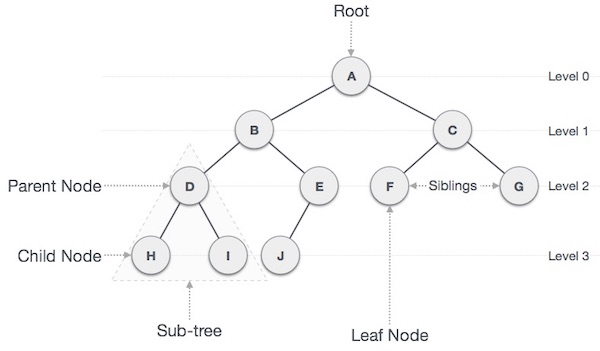
\includegraphics[scale=0.5]{code/sort/pic/binary_tree.jpg}
	\caption{Tree data structure}
\end{figure}

\begin{itemize}
\item \textbf{Root Node}: Root node is the topmost node of a tree. It is always the first node created while creating the tree and we can access each element of the tree starting from the root node.

\item \textbf{Parent node}: The parent of any node is the node which references the current node. 

\item \textbf{Child node}: Child nodes of a parent node are the nodes at which the parent node is pointing using the references.

\item \textbf{Edge}: The reference through which a parent node is connected to a child node is called an edge.

\item \textbf{Leaf node}: These are those nodes in the tree which have no children.

\item \textbf{Siblings}: Nodes with the same parent are called siblings.

\item \textbf{Level}: Level of a node represents the generation of a node. If the root node is at level 0, then its next child node is at level 1, its grandchild is at level 2, and so on.

\item \textbf{Height}: The height of a node is the number of edges on the longest path from the node to a leaf.

\item \textbf{Height of tree}: Height of a tree is the height of its root.

\item \textbf{Depth}: The depth of a node is the number of edges on the path from the root to the node.

\item \textbf{Node degree}: It is the maximum number of children a node has.

\item \textbf{Tree degree}: Tree degree is the maximum of the node degrees.
\end{itemize}

\noindent We can use arrays to represent a hierarchical structure by making array of arrays. For example, for the tree \ref{fig:rep_tree}, the corresponding array will be:
\begin{lstlisting}
T = ['c', ['a', ['p'], ['n'], ['t']], ['o', ['n']]]
\end{lstlisting}

\begin{figure}
    \centering
    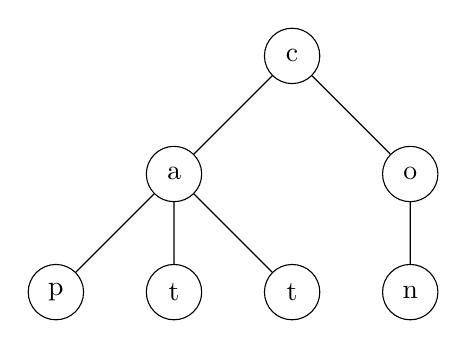
\begin{tikzpicture}[
every node/.style = {minimum width = 2em, draw, circle},
  level/.style = {sibling distance = 30mm/#1}
]
\node {c}
    child {node {a} 
        child {node {p}}
        child {node {t}}
        child {node {t}}
    }
    child {node {o}
        child {node {n}}
        % child {edge from parent[draw = none]}
    };
\end{tikzpicture}
    \caption{A tree used for representing as an array}
    \label{fig:rep_tree}
\end{figure}

% \begin{figure}
%     \centering
%     \begin{tikzpicture}[
% every node/.style = {minimum width = 2em, draw, circle},
%   level/.style = {sibling distance = 40mm/#1}
% ]
% \node {A}
%     child {node {B} 
%         child {node {D}
%             child {node {I}}
%             child {node {J}}
%         }
%         child {node {E}}
%     }
%     child {node {C}
%         child {node {G}}
%         child {node {H}}
%     };
% \end{tikzpicture}
% \end{figure}

\subsection{Binary tree}

\noindent A binary tree is a tree data structure in which each node can have a maximum of 2 children. It means that each node in a binary tree can have either one, or two or no children. We can also classify a binary tree into different categories.
\begin{itemize}
    \item \textbf{Full binary tree}: A binary tree in which every node has 2 children except the leaves is known as a full binary tree.
    \item \textbf{Complete binary tree}: A binary tree in which the last level may not be completely filled and the bottom level is filled from left to right.
    \item \textbf{Perfect binary tree}: In a perfect binary tree, each leaf is at the same level and all the interior nodes have two children. 
\end{itemize}

\subsection{Depth First Search of a Binary tree}
\vspace{5mm}

\noindent DFS (Depth-first search) is technique used for traversing a tree or graph. Here backtracking is used for traversal. In this traversal first the deepest node is visited and then backtracks to it's parent node if no sibling of that node exist. 

\begin{center}
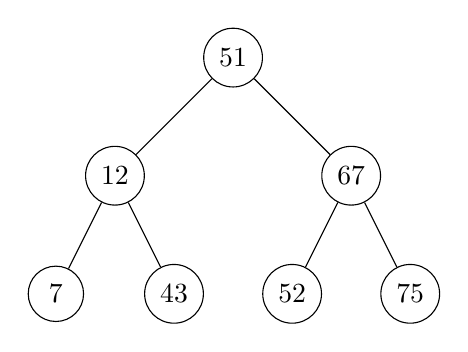
\begin{tikzpicture}[
every node/.style = {minimum width = 2em, draw, circle},
  level/.style = {sibling distance = 30mm/#1}
]
\node {51}
    child {node {12} 
        child {node {7}}
        child {node {43}}
    }
    child {node {67}
        child {node {52}}
        child {node {75}}
    };
\end{tikzpicture}
\end{center}

\noindent There are three ways we can implement the DFS for a Binary tree.

\subsubsection{Pre-order traversal}
        \begin{enumerate}
            \item Visit the root.
            \item Traverse the left subtree, i.e., call Pre-order on left-subtree resursively.
            \item Traverse the right subtree, i.e., call Pre-order on right-subtree recursively.
        \end{enumerate}
        \begin{center}
        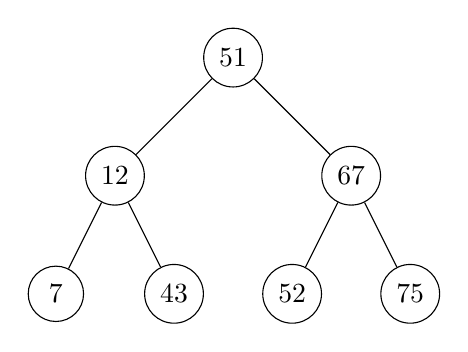
\begin{tikzpicture}[
        every node/.style = {minimum width = 2em, draw, circle},
          level/.style = {sibling distance = 30mm/#1}
        ]
        \node {51}
            child {node {12} 
                child {node {7}}
                child {node {43}}
            }
            child {node {67}
                child {node {52}}
                child {node {75}}
            };
        \end{tikzpicture}
        \vspace{6mm}

        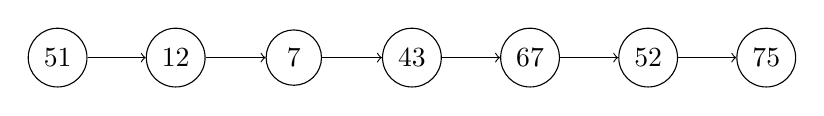
\begin{tikzpicture}[
        every node/.style = {minimum width = 2em, draw, circle, node distance={15mm}},
          level/.style = {sibling distance = 30mm/#1}
        ]
        \node (1) {51};
        \node (2) [right of=1] {12};
        \node (3) [right of=2] {7}; 
        \node (4) [right of=3] {43};
        \node (5) [right of=4] {67};
        \node (6) [right of=5] {52};
        \node (7) [right of=6] {75};
        \draw[->] (1) -- (2);
        \draw[->] (2) -- (3);
        \draw[->] (3) -- (4);
        \draw[->] (4) -- (5);
        \draw[->] (5) -- (6);
        \draw[->] (6) -- (7);
        \end{tikzpicture}
        \end{center}
\subsubsection{In-order traversal}
        \begin{enumerate}
            \item Traverse the left subtree, i.e., call In-order on left-subtree resursively.
            \item Visit the root.
            \item Traverse the right subtree, i.e., call In-order on right-subtree recursively.
        \end{enumerate}
        \begin{center}
        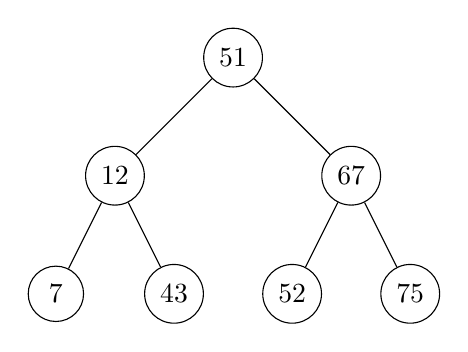
\begin{tikzpicture}[
        every node/.style = {minimum width = 2em, draw, circle},
          level/.style = {sibling distance = 30mm/#1}
        ]
        \node {51}
            child {node {12} 
                child {node {7}}
                child {node {43}}
            }
            child {node {67}
                child {node {52}}
                child {node {75}}
                % child {edge from parent[draw = none]}
            };
        \end{tikzpicture}
        \vspace{6mm}

        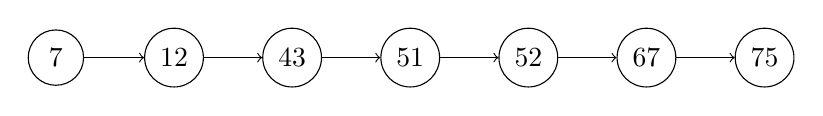
\begin{tikzpicture}[
        every node/.style = {minimum width = 2em, draw, circle, node distance={15mm}},
          level/.style = {sibling distance = 30mm/#1}
        ]
        \node (1) {7};
        \node (2) [right of=1] {12};
        \node (3) [right of=2] {43}; 
        \node (4) [right of=3] {51};
        \node (5) [right of=4] {52};
        \node (6) [right of=5] {67};
        \node (7) [right of=6] {75};
        \draw[->] (1) -- (2);
        \draw[->] (2) -- (3);
        \draw[->] (3) -- (4);
        \draw[->] (4) -- (5);
        \draw[->] (5) -- (6);
        \draw[->] (6) -- (7);
        \end{tikzpicture}
        \end{center}
\subsubsection{Post-order traversal}
        \begin{enumerate}
            \item Traverse the left subtree, i.e., call Post-order on left-subtree resursively.
            \item Traverse the right subtree, i.e., call Post-order on right-subtree recursively.
            \item Visit the root.
        \end{enumerate}
        \begin{center}
        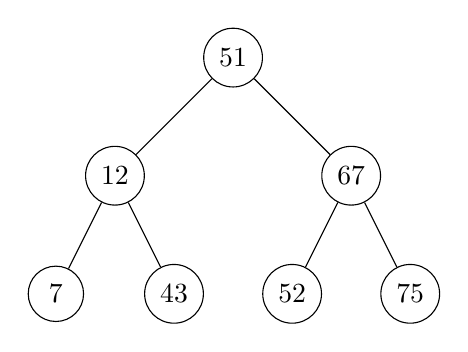
\begin{tikzpicture}[
        every node/.style = {minimum width = 2em, draw, circle},
          level/.style = {sibling distance = 30mm/#1}
        ]
        \node {51}
            child {node {12} 
                child {node {7}}
                child {node {43}}
            }
            child {node {67}
                child {node {52}}
                child {node {75}}
            };
        \end{tikzpicture}
        \vspace{6mm}

        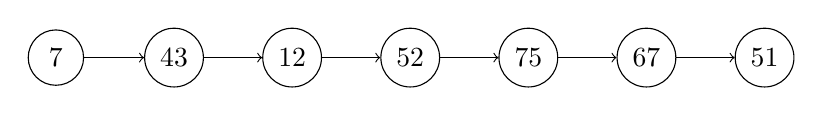
\begin{tikzpicture}[
        every node/.style = {minimum width = 2em, draw, circle, node distance={15mm}},
          level/.style = {sibling distance = 30mm/#1}
        ]
        \node (1) {7};
        \node (2) [right of=1] {43};
        \node (3) [right of=2] {12}; 
        \node (4) [right of=3] {52};
        \node (5) [right of=4] {75};
        \node (6) [right of=5] {67};
        \node (7) [right of=6] {51};
        \draw[->] (1) -- (2);
        \draw[->] (2) -- (3);
        \draw[->] (3) -- (4);
        \draw[->] (4) -- (5);
        \draw[->] (5) -- (6);
        \draw[->] (6) -- (7);
        \end{tikzpicture}
        \end{center}

\noindent Time complexity: $O(n)$

\noindent Space complexity: $O(h)$ where $h$ is the height (maximum depth from root) of the tree

Even if we aren't using any additional data structures, we are using a recursive function, which means that we have to have a look on the maximum number of calls that can be on the call stack, and in this case, it represents the height $h$ of the tree. This is our space complexity.


\begin{lstlisting}
class Tree_node:
	def __init__(self, data, left = None, right = None):
		self.data = data
		self.left = left
		self.right = right

def dfsPreorder(root):
	if root is None:
		return
	print(root.data, end=" ")
	dfsPreorder(root.left)
	dfsPreorder(root.right)
	
def dfsInorder(root):
	if root is None:
		return
	dfsInorder(root.left)
	print(root.data, end=" ")
	dfsInorder(root.right)

def dfsPostorder(root):
	if root is None:
		return
	dfsPostorder(root.left)
	dfsPostorder(root.right)
	print(root.data, end=" ")

def main():
	# Creating the BST
	node_51 = Tree_node(51) # root node of the tree
	node_12 = Tree_node(12)
	node_67 = Tree_node(67)
	node_7 = Tree_node(7)
	node_43 = Tree_node(43)
	node_52 = Tree_node(52)
	node_75 = Tree_node(75)
	node_51.left = node_12
	node_51.right = node_67
	node_12.left = node_7
	node_12.right = node_43
	node_67.left = node_52
	node_67.right = node_75

	# Pre-order traversal
	dfsPreorder(node_51)
	print("\n")
	# In-order traversal
	dfsInorder(node_51)
	print("\n")
	# Post-order traversal
	dfsPostorder(node_51)

if __name__ == "__main__":
	main()
\end{lstlisting}
Output
\begin{lstlisting}
51 12 7 43 67 52 75 
7 12 43 51 52 67 75 
7 43 12 52 75 67 51
\end{lstlisting}

\subsection{Breadth First Search of a Tree}
\vspace{5mm}
\noindent Breadth-first search (BFS) also known as \textit{Level-order traversal} is a tree or graph traversal algorithm that starts traversing from the root node and explores all the child nodes.
\vspace{5mm}

\noindent \textbf{Using Queue (Iterative approach)}: For each node, first the node is visited and then it's child nodes are put in a FIFO queue.

\begin{enumerate}
    \item Create an empty queue.
    \item Push root node into queue.
    \item Loop while queue is not empty:
    \begin{enumerate}
        \item Pop a node from queue.
        \item Print the associated data.
        \item Push the node's children 
        (first left then right children for binary tree) into queue if any.
    \end{enumerate}
\end{enumerate}

\begin{center}
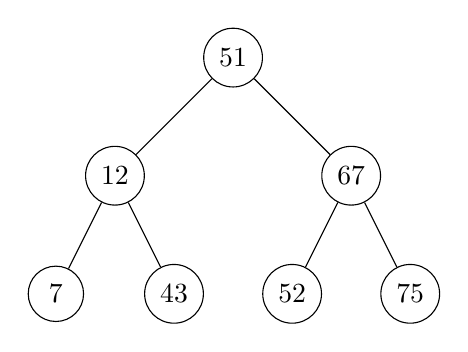
\begin{tikzpicture}[
every node/.style = {minimum width = 2em, draw, circle},
  level/.style = {sibling distance = 30mm/#1}
]
\node {51}
    child {node {12} 
        child {node {7}}
        child {node {43}}
    }
    child {node {67}
        child {node {52}}
        child {node {75}}
        % child {edge from parent[draw = none]}
    };
\end{tikzpicture}
\vspace{6mm}

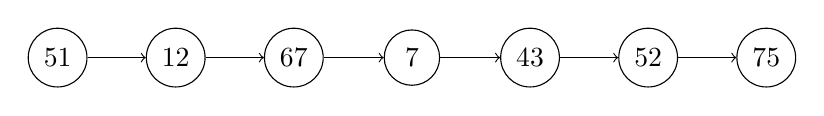
\begin{tikzpicture}[
every node/.style = {minimum width = 2em, draw, circle, node distance={15mm}},
  level/.style = {sibling distance = 30mm/#1}
]
\node (1) {51};
\node (2) [right of=1] {12};
\node (3) [right of=2] {67}; 
\node (4) [right of=3] {7};
\node (5) [right of=4] {43};
\node (6) [right of=5] {52};
\node (7) [right of=6] {75};
\draw[->] (1) -- (2);
\draw[->] (2) -- (3);
\draw[->] (3) -- (4);
\draw[->] (4) -- (5);
\draw[->] (5) -- (6);
\draw[->] (6) -- (7);
\end{tikzpicture}
\end{center}

\noindent Time complexity: $O(n)$

\noindent Space complexity: $O(n)$

\vspace{5mm}

\noindent \textbf{Using Queue (Recursive approach)}: 

\begin{enumerate}
    \item If the queue is not empty do the following:
    \begin{enumerate}
        \item Pop a node from queue.
        \item Print the associated data.
        \item Push the node's children 
        (first left then right children for binary tree) into queue if any.
    \end{enumerate}
    \item Recursively call the function with the new state of queue.
\end{enumerate}

\noindent Time complexity: $O(n)$

\noindent Space complexity: $O(n)$

\begin{lstlisting}
class Tree_node:
    def __init__(self, data, left = None, right = None):
        self.data = data
        self.left = left
        self.right = right

def LevelOrder(root):
    # Base Case
    if root is None:
        return
        
    # Create an empty queue
    queue = []
 
    # Enqueue Root
    queue.append(root)
 
    while(len(queue) > 0):
        # Remove the first node from queue and print the associated data
        node = queue.pop(0)
        print(node.data, end=" ")
 
        # Enqueue left child
        if node.left is not None:
            queue.append(node.left)
 
        # Enqueue right child
        if node.right is not None:
            queue.append(node.right)
            
def LevelOrderRecursive(root, queue):
	# Base Case
    if root is None:
        return

    if len(queue) == 0:
        return
    else:
        # Remove the first node from queue and print the associated data
        node = queue.pop(0)
        print(node.data, end=" ")

        # Enqueue left child
        if node.left is not None:
            queue.append(node.left)

        # Enqueue right child
        if node.right is not None:
            queue.append(node.right)

    LevelOrderRecursive(root, queue)

def main():
    # Creating the BST
    node_51 = Tree_node(51) # root node of the tree
    node_12 = Tree_node(12)
    node_67 = Tree_node(67)
    node_7 = Tree_node(7)
    node_43 = Tree_node(43)
    node_52 = Tree_node(52)
    node_75 = Tree_node(75)
    node_51.left = node_12
    node_51.right = node_67
    node_12.left = node_7
    node_12.right = node_43
    node_67.left = node_52
    node_67.right = node_75
    
    # Level-order traversal (Iterative approach)
    LevelOrder(node_51)
    print()
    # Level-order traversal (Recursive approach)
    LevelOrderRecursive(node_51, [node_51])

if __name__ == "__main__":
    main()
\end{lstlisting}
Output
\begin{lstlisting}
51 12 67 7 43 52 75
51 12 67 7 43 52 75
\end{lstlisting}

\section{Binary Search Tree (BST)}

A Binary search Tree (BST) is one data structure that supports faster searching, rapid sorting and easy insertion and deletion. A BST is a sorted version of Binary tree. A tree whose elements have at most 2 children is called a binary tree. The ordering of BST is also referred to as BST property. A BST must have the following properties:
\begin{enumerate}
\item The left subtree of a node contains only nodes with keys less than the node's key.
\item The right subtree of a node contains only nodes with keys greater than the node's key.
\item Duplicate keys are not allowed.
\end{enumerate}

\begin{center}
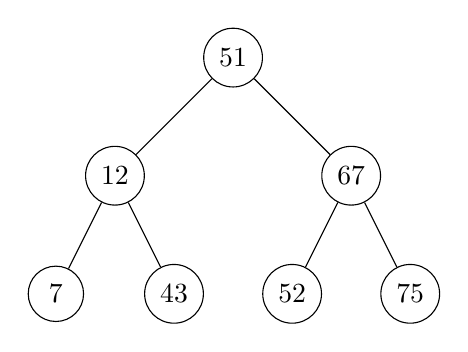
\begin{tikzpicture}[
every node/.style = {minimum width = 2em, draw, circle},
  level/.style = {sibling distance = 30mm/#1}
]
\node {51}
    child {node {12} 
        child {node {7}}
        child {node {43}}
    }
    child {node {67}
        child {node {52}}
        child {node {75}}
        % child {edge from parent[draw = none]}
    };
\end{tikzpicture}
\end{center}

\textbf{Advantages of Binary search tree}
\begin{enumerate}
    \item Searching an element in the Binary search tree is easy and fast ($\sim O(\log n)$) as we always have a hint that which subtree has the desired element.
    \item As compared to array and linked lists, insertion and deletion operations are faster ($\sim O(\log n)$) in BST.
\end{enumerate}

\textbf{Disdvantages of Binary search tree}
\begin{enumerate}
    \item The shape of the binary search tree totally depends on the order of insertions, and it can degenerate.
    \item The main disadvantage is that we should always implement a balanced binary search tree - AVL tree, Red-Black tree, Splay tree. Otherwise the cost of operations may not be logarithmic and degenerate into a linear search on an array.
    \item Duplicate values cannot be inserted.
\end{enumerate}

\subsection{Insertion operation}

\noindent Iterative method: 
\begin{enumerate}
    \item Set the \lstinline{currentNode} pointer to the root node. 
    \item Compare the data to be inserted with the \lstinline{currentNode}'s data.
    \item If the data is smaller, move the \lstinline{currentNode} pointer to the left child if it exist. If it does not exist, insert it as the left child of the \lstinline{currentNode}.
    \item If the data is larger, move the \lstinline{currentNode} pointer to the right child if it exist. If it does not exist, insert it as the right child of the \lstinline{currentNode}.
    \item Repeat the steps (2), (3) and (4) till the node is inserted.
\end{enumerate} 
\begin{lstlisting}
class BSTNode():
    # Constructor
    def __init__(self, data):
        self.data = data
        self.left = None
        self.right = None
        
    # Insert a New Node in a Binary Search Tree 
    def insert(self, data):
        # If the self.data is None, create a new node
        if not self.data:
            self.data = data
            return

        # Duplicate value not added
        if self.data == data:
            return

        currentNode = self
        while True:
            if data < currentNode.data:
                # If there is no left child, insert the node on the left
                if not currentNode.left:
                    currentNode.left = BSTNode(data)
                    return
                # Move the currentNode pointer to the left child
                currentNode = currentNode.left
            else:
                # If there is no right child, insert the node on the right
                if not currentNode.right:
                    currentNode.right = BSTNode(data)
                    return
                # Move the currentNode pointer to the right child
                currentNode = currentNode.right
                
if __name__ == '__main__':
    root = BSTNode(8)
    root.insert(11)
    root.insert(14)
    root.insert(5)
    root.insert(1)
    root.insert(6)

    root.display() 
\end{lstlisting}
\textbf{Output} \footnote{Here display() is a method of the BSTNode class which is not shown in the code. It will just display the all the nodes in tree structure in the console.}
\begin{lstlisting}
  _8_   
 /   \  
 5  11_ 
/ \    \
1 6   14
\end{lstlisting}

\noindent Recursive method: 

\begin{itemize}
    \item Starting from the root node, compare the data to be inserted with the root node's data.
    \item If the data is smaller, recursively call insert for the left subtree if it exists. If it does not exist, then attach it as as the left child.
    \item If the data is larger, recursively call insert for the right subtree if it exists. If it does not exist, then attach it as as the right child.
\end{itemize} 

\begin{lstlisting}
class BSTNode():
    # Constructor
    def __init__(self, data):
        self.data = data
        self.left = None
        self.right = None
        
    # Insert a New Node in a Binary Search Tree 
    def insertRec(self, data):
        # If the self.data is None, create a new node
        if not self.data:
            self.data = data
            return

        # Duplicate value not added
        if self.data == data:
            return

        # If the given data is less than the self node, 
        # Then if self.left exist, recur for the left subtree
        # Else add the node as the left child to the self node.
        if data < self.data:
            if self.left:
                self.left.insertRec(data)
                return
            self.left = BSTNode(data)
        # If the given data is less than the self node, 
        # Then if self.right exist, recur for the right subtree
        # Else add the node as the right child to the self node.
        else:
            if self.right:
                self.right.insertRec(data)
                return
            self.right = BSTNode(data)
                
if __name__ == '__main__':
    root = BSTNode(8)
    root.insertRec(11)
    root.insertRec(14)
    root.insertRec(5)
    root.insertRec(1)
    root.insertRec(6)

    root.display() 
\end{lstlisting}
\textbf{Output} \footnote{Here display() is a method of the BSTNode class which is not shown in the code. It will just display the all the nodes in tree structure in the console.}
\begin{lstlisting}
  _8_   
 /   \  
 5  11_ 
/ \    \
1 6   14
\end{lstlisting}

\subsection{Search operation}

\noindent Iterative method:
\begin{itemize}
    \item Set the \lstinline{currentNode} pointer to the root node. 
    \item Compare the data to be searched with the \lstinline{currentNode}'s data.
    \item If the data is smaller, move the \lstinline{currentNode} pointer to the left child.
    \item If the data is larger, move the \lstinline{currentNode} pointer to the right child.
    \item Repeat the steps (2), (3) and (4) till the searched node is found or \lstinline{currentNode} is Null.
    \item Return the \lstinline{currentNode}.
\end{itemize}

\begin{lstlisting}
class BSTNode():
    # Constructor
    def __init__(self, data):
        self.data = data
        self.left = None
        self.right = None
       
    # Find a Node in a BST 
    def findNode(self, data):
        # If the self.data is None, return None
        if not self.data:
            return None
        
        currentNode = self
        while data != currentNode.data:
            # If the data is less than the currentNode's data, move the currentNode pointer to the left child
            if data < currentNode.data:
                currentNode = currentNode.left
            # If the data is greater than the currentNode's data, move the currentNode pointer to the right child
            else:
                currentNode = currentNode.right
            # If no match
            if currentNode is None: 
                return None
        # In case the self node contains the searched data, the while loop will be skipped altogether and the self node will be returned.
        return currentNode
        
if __name__ == '__main__':
    root = BSTNode(8)
    root.insertRec(11)
    root.insertRec(14)
    root.insertRec(5)
    root.insertRec(6)
    root.insertRec(1)
    
    foundNode = root.findNode(7)
    if foundNode is None:
        print("Could not find the node.")
    else:
        print("Found the node.")
\end{lstlisting}
\textbf{Output}
\begin{lstlisting}
Could not find the node.
\end{lstlisting}

\noindent Recursive method:

\begin{lstlisting}
class BSTNode():
    # Constructor
    def __init__(self, data):
        self.data = data
        self.left = None
        self.right = None
       
    # Find a Node in a BST 
    def findNodeRec(self, data):
        # If the self.data is None, return None
        if not self.data:
            return None

        # If the data is less than the root's data, recursively call the left subtree
        if data < self.data:
            if self.left:
                return self.left.findNodeRec(data)
            return None
        # If the data is greater than the root's data, recursively call the right subtree
        elif data > self.data:
            if self.right:
                return self.right.findNodeRec(data)
            return None
        # Return self if self.data matches with the data
        else:
            return self
        
if __name__ == '__main__':
    root = BSTNode(8)
    root.insertRec(11)
    root.insertRec(14)
    root.insertRec(5)
    root.insertRec(6)
    root.insertRec(1)
    
    foundNode = root.findNodeRec(7)
    if foundNode is None:
        print("Could not find the node.")
    else:
        print("Found the node.")
\end{lstlisting}
\textbf{Output}
\begin{lstlisting}
Found the node.
\end{lstlisting}

\subsection{Finding the min and max value}

\noindent The left-most leaf node of the tree contains the minimum value while the right-most leaf node of the tree contains the maximum value.

\begin{lstlisting}
class BSTNode():
    # Constructor
    def __init__(self, data):
        self.data = data
        self.left = None
        self.right = None
    
    # Get the Minimum Value in a BST 
    # The left most value is the Smallest Value
    def getMinValue(self):
        currentNode = self
        while currentNode.left is not None:
            currentNode = currentNode.left
        return currentNode.data
        
    # Get the Maximum Value in a BST 
    # The right most value is the Maximum Value
    def getMaxValue(self):
        currentNode = self
        while True:
            if not currentNode.right:
                return currentNode.data
            currentNode = currentNode.right

if __name__ == '__main__':
    root = BSTNode(8)
    root.insertRec(11)
    root.insertRec(14)
    root.insertRec(5)
    root.insertRec(6)
    root.insertRec(1)
    
    print('Min value:', root.getMinValue())
    print('Max value:', root.getMaxValue())
\end{lstlisting}
\textbf{Output}
\begin{lstlisting}
Min value: 1
Max value: 14
\end{lstlisting}

\subsection{Height and size of BST}

\noindent The \textit{height/depth} of a binary tree is defined as the length of the longest path from its root node to a leaf. 

\noindent The \textit{size} of a binary tree is defined as the number of nodes in the tree.

\begin{lstlisting}
class BSTNode():
    # Constructor
    def __init__(self, data):
        self.data = data
        self.left = None
        self.right = None
        
    # Computation of height/depth of a binary tree
    def tree_height(self):
        if self.data is None:
            return 0
        if self.left:
            height_of_left_subtree = self.left.tree_height()
        else:
            height_of_left_subtree = 0
        if self.right:
            height_of_right_subtree = self.right.tree_height()
        else:
            height_of_right_subtree = 0
        return 1 + max(height_of_left_subtree, height_of_right_subtree)

    # Computation of number of nodes in a binary tree
    def tree_size(self):
        if self.data is None:
            return 0
        if self.left:
            size_of_left_subtree = self.left.tree_size()
        else:
            size_of_left_subtree = 0
        if self.right:
            size_of_right_subtree = self.right.tree_size()
        else:
            size_of_right_subtree = 0
        return 1 + size_of_left_subtree + size_of_right_subtree
        
if __name__ == '__main__':
    root = BSTNode(8)
    root.insert(11)
    root.insert(14)
    root.insert(5)
    root.insert(1)
    root.insert(6)
    root.insert(9)
    root.insert(16)

    root.display()
    
    print('Height of the tree:', root.tree_height())
    print('Size of the tree:', root.tree_size())
\end{lstlisting}
\textbf{Output}
\begin{lstlisting}
  _8__     
 /    \    
 5   11_   
/ \ /   \  
1 6 9  14_ 
          \
         16
Height of the tree: 4
Size of the tree: 8
\end{lstlisting}

\subsection{Finding the parent node}

\begin{enumerate}
    \item If the data is found in the root node then there is no parent node for that. So return Null.
    \item Create a pointer \lstinline{currentNode} to point to the root.
    \item If the data is smaller than the \lstinline{currentNode}'s data, move the pointer to the left child after saving the parent node in a separate pointer called \lstinline{parentNode}.
    \item If the data is larger than the \lstinline{currentNode}'s data, move the pointer to the right child after saving the parent node in a separate pointer called \lstinline{parentNode}.
    \item Repeat the steps (3) and (4) until the \lstinline{currentNode} contains the given data or \lstinline{currentNode} points to Null. In the first case return the Node pointed by \lstinline{parentNode}. In the second case return Null.
\end{enumerate}
\begin{lstlisting}
class BSTNode():
    # Constructor
    def __init__(self, data):
        self.data = data
        self.left = None
        self.right = None
        
    # Find the parent node
    def findParentNode(self, data):
        if data == self.data:
            return None # Data found at root node, no parent
        currentNode = self
        while  data != currentNode.data:
            if data < currentNode.data:
                parentNode = currentNode # Saving the parent node
                currentNode = currentNode.left
            else:
                parentNode = currentNode
                currentNode = currentNode.right
            if currentNode is None: # data is not found
                return None
        return parentNode
if __name__ == '__main__':
    root = BSTNode(8)
    root.insert(11)
    root.insert(14)
    root.insert(5)
    root.insert(1)
    root.insert(6)
    root.insert(9)
    root.insert(16)

    root.display()
    
    foundNode = root.findParentNode(6)
    if foundNode is None:
        print("Could not find the parent node.")
    else:
        print(f"The data in the parent node is {foundNode.data}.")
\end{lstlisting}
\textbf{Output}
\begin{lstlisting}
  _8__     
 /    \    
 5   11_   
/ \ /   \  
1 6 9  14_ 
          \
         16
The data in the parent node is 5.
\end{lstlisting}

\subsection{Successor and Predecessor}

\noindent If we sort the nodes of a BST based on the data in increasing order (in-order walk), each node is the \textit{successor} of the preceding node. Similarly, each node is the \textit{predecessor} of the following node.

\noindent To find the successor of a node \lstinline{x}, we do the following:
\begin{enumerate}
\item If the right subtree of node \lstinline{x} is non-empty, then the successor of \lstinline{x} is just the leftmost node in \lstinline{x}'s right subtree.
\item If the right subtree of node \lstinline{x} is empty, then move towards parent nodes, untill the node \lstinline{x} becomes a part of the left subtree of some parent node \lstinline{y} for the first time. If such node \lstinline{y} exist, then it is the successor of node \lstinline{x}.
\end{enumerate}

\begin{center}
    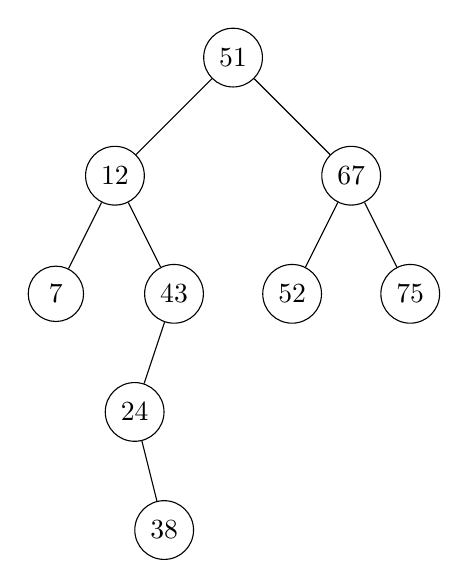
\begin{tikzpicture}[
every node/.style = {minimum width = 2em, draw, circle},
  level/.style = {sibling distance = 30mm/#1}
]
\node {51}
    child {node {12} 
        child {node {7}}
        child {node {43}
            child { node {24}
                child {edge from parent[draw = none]}
                child { node {38}}
            }
            child {edge from parent[draw = none]}
        }
    }
    child {node {67}
        child {node {52}}
        child {node {75}}
        % child {edge from parent[draw = none]}
    };
\end{tikzpicture}
\end{center}

% \vspace{5mm}
In-order walk: $ 7 \rightarrow  12 \rightarrow  24 \rightarrow  38 \rightarrow  43 \rightarrow  51 \rightarrow  52 \rightarrow  67 \rightarrow  75 $

% \begin{center}
% \begin{tikzpicture}[
%         every node/.style = {minimum width = 2em, draw, circle, node distance={12mm}},
%           level/.style = {sibling distance = 30mm/#1}
%         ]
%         \node (1) {7};
%         \node (2) [right of=1] {12};
%         \node (3) [right of=2] {24}; 
%         \node (4) [right of=3] {38};
%         \node (5) [right of=4] {43};
%         \node (6) [right of=5] {51};
%         \node (7) [right of=6] {52};
%         \node (8) [right of=7] {67};
%         \node (9) [right of=8] {75};
%         \draw[->] (1) -- (2);
%         \draw[->] (2) -- (3);
%         \draw[->] (3) -- (4);
%         \draw[->] (4) -- (5);
%         \draw[->] (5) -- (6);
%         \draw[->] (6) -- (7);
%         \draw[->] (7) -- (8);
%         \draw[->] (8) -- (9);
%         \end{tikzpicture}
% \end{center}
\vspace{5mm} 

\noindent Here in the picture, the successor of node \circled{12} is node \circled{24}. The successor of node \circled{43} is node \circled{51}. 

\vspace{5mm}

\noindent In a similar way, to find the predecessor of a node \lstinline{x}, we do the following:
\begin{enumerate}
\item If the left subtree of node \lstinline{x} is non-empty, then the successor of \lstinline{x} is just the rightmost node in \lstinline{x}'s left subtree.
\item If the left subtree of node \lstinline{x} is empty, then move towards parent nodes, untill the node \lstinline{x} becomes a part of the right subtree of some parent node \lstinline{y} for the first time. If such node \lstinline{y} exist, then it is the predecessor of node \lstinline{x}.
\end{enumerate}

\noindent Here in the previous picture, the predecessor of node \circled{43} is node \circled{38}. The predecessor of node \circled{24} is node \circled{12}.

\vspace{5mm}

\begin{lstlisting}
def findSuccessor(x):
    # If the right subtree of node x is non-empty, then the successor of x is just the left most node in x's right subtree
    if x.right is not None:
        temp = x.right
        while temp.left:
            temp = temp.left
        return temp
    # If the right subtree of node x is empty, then move towards parentnodes, untill the node x becomes a part of the left subtree of some parent node y for the first time. 
    else:
        # We need to have a parent pointer in the BSTNode, else we have to traverse the entire tree.
        y = x.parent
        while (y != None) and (x == y.right):
            x = y
            y = y.parent
    return y


def findPredecessor(x):
    # If the right subtree of node x is non-empty, then the predecessor of x is just the right most node in x's left subtree
    if x.left is not None:
        temp = x.left
        while temp.right:
            temp = temp.right
        return temp
    # If the left subtree of node x is empty, then move towards parent nodes, untill the node x becomes a part of the right subtree of some parent node y for the first time. 
    else:
        # We need to have a parent pointer in the BSTNode, else we have to traverse the entire tree.
        y = x.parent
        while (y != None) and (x == y.left):
            x = y
            y = y.parent
    return y
\end{lstlisting}

\subsection{Delete operation}

\noindent Deletion of an element involves a slightly complicated operation than insertion of an element. Three cases exist with respect to the deletion of a node:

\begin{itemize}
    \item \textbf{Case 1: If the node to be deleted is a leaf node}.
    
    This is the simplest case. The leaf element can be deleted directly.
    \item \textbf{Case 2: If the node to be deleted has only one child}.
    
    In this case the element has to be replaced by the child node.
    \item \textbf{Case 3: If the node to be deleted has two children}.
    
    In this case the largest key in the left subtree (inorder successor) has to be found, which will replace the element to be deleted. Alternatively, the smallest key in the right subtree (inorder predecessor) has to be found, which will replace the element to be deleted.
\end{itemize}

\begin{lstlisting}
class BSTNode():
    # Constructor
    def __init__(self, data):
        self.data = data
        self.left = None
        self.right = None
        
    def findsuccessor(self):
        # If the right subtree of node current_node is non-empty, then the successor of current_node is just the left most node in current_node's right subtree
        if self.right is not None:
            temp = self.right
            while temp.left:
                temp = temp.left
        return temp

    def deleteNode(self, data):
        # Base Case
        if self.data is None:
            return self
    
        # If the data to be deleted is smaller than the self's data then it lies in left subtree
        if data < self.data:
            if self.left:
                self.left = self.left.deleteNode(data)
    
        # If the data to be delete is greater than the self's data then it lies in right subtree
        elif(data > self.data):
            if self.right:
                self.right = self.right.deleteNode(data)
    
        # If data is same as self's data, then this is the node
        # to be deleted
        else:
            # Case 1: Leaf node
            if (self.left is None) and (self.right is None):
                self = None
                return None

            # Case 2: Node with only one child 
            if self.left is None:
                # Left child
                temp = self.right
                self = None
                return temp
    
            elif self.right is None:
                # Right child
                temp = self.left
                self = None
                return temp
    
            # Case 3: Node with two children:
            else:
                # Get the inorder successor
                # (smallest node in the right subtree)
                temp = self.findsuccessor()
                # Copy the inorder successor's content to this node
                self.data = temp.data
        
                # Delete the inorder successor
                self.right = self.right.deleteNode(temp.data)
    
        return self
        
if __name__ == '__main__':
    root = BSTNode(8)
    root.insert(11)
    root.insert(14)
    root.insert(5)
    root.insert(1)
    root.insert(6)
    root.insert(9)
    root.insert(16)

    root.display()
    
    root.deleteNode(16)
    print('After deleting node 16 (leaf node)')
    root.display()
    root.deleteNode(1)
    print('After deleting node 1 (one child)')
    root.display()
    root.deleteNode(8)
    print('After deleting node 8 (two children)')
    root.display()
\end{lstlisting}
\textbf{Output}
\begin{lstlisting}
  _8__     
 /    \    
 5   11_   
/ \ /   \  
1 6 9  14_ 
          \
         16
After deleting node 1 (leaf node)
 _8__     
/    \    
5   11_   
 \ /   \  
 6 9  14_ 
         \
        16
After deleting node 14 (one child)
 _8__   
/    \  
5   11_ 
 \ /   \
 6 9  16
After deleting node 8 (two children)
 _9_   
/   \  
5  11_ 
 \    \
 6   16
\end{lstlisting}

\newpage
\section{Hash table}



% Hash table (a.k.a Hash map) is one of the most important data structures that maps a given value with a key to access the elements faster in $O(1)$ time. The information stored in a hash table has basically two main components, i.e., \textit{key} and \textit{value}. The hash table can be implemented with the help of an associative array. The efficiency depends upon the efficiency of the hash function used for mapping. For example, suppose the key value is `John' and the value is the phone number $9893260037$. We pass the key value in the hash function $H(.)$ to generate an index. For example,

% $$\text{Hash(`John')} = 3$$

% \noindent The value i.e. the phone number $9893260037$ corresponding to that key is stored in the index.  Ideal hashing should produce a different index for each key. However, \textbf{collisions} can occur whenever hash function produces the same index for multiple keys. The time complexity in hashing is $O(1)$.

\noindent A hash table (a.k.a Hash map) is an important data structure which stores data based on key-value pairs in such a way as to access the elements faster in $O(1)$ time. Each position of the hash table, often called a \textbf{slot}, can hold an item and is indexed by an integer value starting at 0. For example, we will have a slot at index 0, a slot at index 1, a slot at index 2, and so on. Initially, the hash table contains no items so every slot is empty. We can implement a hash table by using a list with each element initialized to the special Python value \lstinline{None}. The following figure shows a hash table of size $m=11$. In other words, there are $m$ slots in the table, at index 0 through 10.

\begin{center}
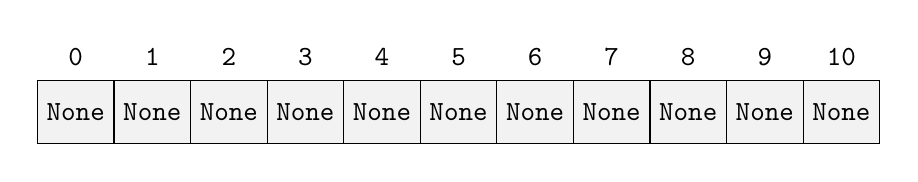
\begin{tikzpicture}[font=\ttfamily,
array/.style={matrix of nodes,nodes={draw, minimum size=8mm, fill=gray!10},column sep=-\pgflinewidth, row sep=0.5mm, nodes in empty cells,
row 1/.style={nodes={draw=none, fill=none, minimum size=5mm}}}]
\matrix[array] (array) {
0 & 1 & 2 & 3 & 4 & 5 & 6 & 7 & 8 & 9 & 10\\
None & None & None & None & None & None & None & None & None & None & None\\};
\end{tikzpicture}
\end{center}

\noindent The mapping between an item (a key-value pair) and the slot is called the \textbf{hash function}. The hash function will take the key of any item in the collection and return an integer in the range of slot indices, between 0 and $m-1$. Assume that we have the set of integers 54, 26, 93, 17, 77, and 31 as keys and their respective values as V54, V26, V93, V17, V77, and V31. Our first hash function, sometimes referred to as the \textbf{remainder method}, simply takes a key and divides it by the table size, returning the remainder as its hash value $$h(\text{key})=\text{key} \% 11$$
\begin{lstlisting}
Key      Hash Value
54        54 % 11 = 10
26        26 % 11 = 4
93        93 % 11 = 5
17        17 % 11 = 6
77        77 % 11 = 0
31        31 % 11 = 9
\end{lstlisting}

\noindent Once the hash values have been computed, we can insert each item into the hash table at the index position given bu the computed hash value as shown in Figure 5. Note that 6 out of 11 slots are now occupied. This is referred to as the \textbf{load factor} $\lambda$, and is commonly defined as $$\lambda=\dfrac{\text{number of items}}{\text{table size}}$$

\begin{center}
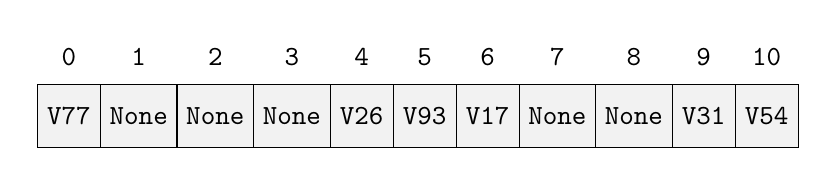
\begin{tikzpicture}[font=\ttfamily,
array/.style={matrix of nodes,nodes={draw, minimum size=8mm, fill=gray!10},column sep=-\pgflinewidth, row sep=1mm, nodes in empty cells,
row 1/.style={nodes={draw=none, fill=none, minimum size=5mm}}}]
\matrix[array] (array) {
0 & 1 & 2 & 3 & 4 & 5 & 6 & 7 & 8 & 9 & 10\\
V77 & None & None & None & V26 & V93 & V17 & None & None & V31 & V54 \\};
\end{tikzpicture}
\end{center}

\noindent Now when we want to search for an item, we simply use the hash function to compute the slot name for the item and then check the hash table to see if it is present. This searching operation is $O(1)$.

\noindent this technique is going to work only if each item maps to a unique location in the hash table. For example, if the item 44 had been the next item in our collection, it would have a hash value of 0 ($44\%11=0$). Since 77 also had a hash value of 0, we would have a problem. According to the hash function, two or more items would need to be in the same slot. This is referred to as a \textbf{collision}.

\begin{lstlisting}
# Python program to demonstrate working of Hash-table 
CAPACITY = 10
hashTable = [None,] * CAPACITY

def hashFunction(key):
    return key % CAPACITY

def insertData(key, data):
    index = hashFunction(key)
    hashTable[index] = [key, data]

def removeData(key):
    index = hashFunction(key)
    hashTable[index] = 0

if __name__ == "__main__":
    print(hashTable)
    insertData(123, "apple")
    insertData(432, "mango")
    insertData(213, "banana")
    insertData(654, "guava")

    print(hashTable)

    removeData(123)

    print(hashTable)
\end{lstlisting}
\textbf{Output}
\begin{lstlisting}
[None, None, None, None, None, None, None, None, None, None]
[None, None, [432, 'mango'], [213, 'banana'], [654, 'guava'], None, None, None, None, None]
[None, None, [432, 'mango'], 0, [654, 'guava'], None, None, None, None, None]
\end{lstlisting}

\subsection{Hashing function}

\noindent The most important part of a hash table is the \textbf{hash function}. The hash function converts a specified key into an index for an array that stores all the data. The three primary requirements for a good hash function are as follows:
\begin{enumerate}
    \item Deterministic: Same keys produce same hash values.
    \item Efficiency: Should be computed in $O(1)$ time.
    \item Collision resistant: A good hash function may not prevent the collisions completely however it can reduce the number of collisions.
    \item Uniform distribution: A non-uniform distribution increases the number of collisions and the cost of resolving them.
\end{enumerate}

\noindent There are many hash functions that use numeric or alphanumeric keys.
\begin{enumerate}
    \item \textbf{Division method}: This is the most simple and easiest method to generate a hash value. If $k$ is the key and $M$ is the size of the hash table, then the hash formula is
    $$h(k) = k\mod M$$
    \noindent It is best suited that $M$ is a prime number as that can make sure the keys are more uniformly distributed. The hash function is dependent upon the remainder of a division.
    \begin{lstlisting}
    k = 12345
    M = 95
    h(12345) = 12345 mod 95 = 90
    \end{lstlisting}
    Pros:
    \begin{enumerate}
        \item The division method is very fast since it requires only a single division operation.
    \end{enumerate}
    Cons:
    \begin{enumerate}
        \item This method leads to poor performance since consecutive keys map to consecutive hash values in the hash table.
        \item Sometimes extra care should be taken to chose value of $M$.
    \end{enumerate}
    
    \item \textbf{Mid square method}: It involves two steps to compute the hash value: (1) Square the value of the key $k$ i.e. $k^2$, (2) Extract the middle $r$ digits as the hash value.
    $$h(k) = \text{middle } r \text{ digits of } k^2$$
    \noindent The value $r$ is decided based on the size of the table.
    \begin{lstlisting}
    k = 60
    k^2 = 60 x 60 = 3600
    h(60) = 60
    \end{lstlisting}
    Pros:
    \begin{enumerate}
        \item The performance of this method is good as most or all digits of the key value contribute to the result.
        \item The result is not dominated by the distribution of the top digit or bottom digit of the original key value.
    \end{enumerate}
    Cons:
    \begin{enumerate}
        \item The size of the key is one of the limitations of this method, as the key is of big size then its square will double the number of digits.
        \item Another disadvantage is that there will be collisions.
    \end{enumerate}
    
    \item \textbf{Digit folding method}: This method involves two steps:
    \begin{enumerate}
        \item Divide the key $k$ into a number of parts i.e. $k_1, k_2, k_3,\cdots k_n$, where each part has the same number of digits except for the last part that can have lesser digits than the other parts.
        \item Add the individual parts. The hash value is obtained by ignoring the last carry if any.
    \end{enumerate}
    
    \begin{lstlisting}
    k = 12345
    k1 = 12, k2 = 34, k3 = 5
    s = k1 + k2 + k3 = 12 + 34 + 5 = 51 
    h(k) = 51
    \end{lstlisting}
    
    \item \textbf{Multiplication method}: This method involves the following steps:
    \begin{enumerate}
        \item Choose a constant value $A$ such that $0 < A < 1$.
        \item Multiply the key with $A$.
        \item Extract the fractional part of $kA$.
        \item Multiply the result of the above step by the size of the hash table i.e. $M$.
        \item The resulting hash value is obtained by taking the floor of the result obtained in step 4.
    \end{enumerate}
    $$h(k) = \lfloor (M (kA \mod 1))\rfloor$$
    \begin{lstlisting}
    k = 12345
    A = 0.357840
    M = 100
    
    h(12345) = floor[ 100 (12345*0.357840 mod 1)]
             = floor[ 100 (4417.5348 mod 1) ]
             = floor[ 100 (0.5348) ]
             = floor[ 53.48 ]
             = 53
    \end{lstlisting}
\end{enumerate}

\subsection{Hash collision}

\noindent When the hash function generates the same index for multiple keys, there will be a conflict (what value to be stored in that index). This is called a hash collision. We can resolve the hash collision using one of the following techniques.
\begin{enumerate}
    \item \textbf{Collision resolution by chaining}: If a hash function produces the same index for multiple elements, these elements are stored in the same index by using a linked list. If $j$ is the slot for multiple elements, it contains a pointer to the head of the list of elements. If no element is present, $j$ contains \lstinline{NULL}.
    \item \textbf{Open Addressing}: Unlike chaining, open addressing doesn't store multiple elements into the same slot. Here, each slot is either filled with a single key or left with \lstinline{NULL}. Different techniques used in open addressing are:
    \begin{enumerate}
        \item \textit{Linear probing}: Linear probing works by finding the next available slot by incrementing one index at a time. A disadvantage to linear probing is the tendency for clustering; items become clustered in the table. When inserting a new element, the entire cluster must be traversed. This adds to the time required to perform operations on the hash table.
        \item \textit{Quadratic probing}: It is a variation to linear probing. Instead of using a constant 'skip' value, we skip the slots using a quadratic formula. This means that if the first hash value is $h$, the successive values are $h+1^2$, $h+2^2$, $h+3^2$, $h+4^2$, and so on. This technique addresses the clustering issue and also helps to evenly distribute across available indices.
        \item \textit{Double hashing}: Another great way to uniformly distribute the keys is by having a second hashing function that hashes the result from the original. 
    \end{enumerate}
    
\end{enumerate}

\newpage
\section{Heap}\label{sec:heap}

\noindent Heap (`binary heap' to be specific) data structure is a \textit{complete binary tree}\footnote{A \textit{complete binary tree} is a binary tree in which all the levels are completely filled except possibly the lowest one, which is filled from the left.} that satisfies the heap property, where any given node is
\begin{itemize}
    \item always greater than its child node(s). This property is also called \textbf{max heap property}. The root node is the largest among all other nodes.
    \item always smaller than the child node(s). This property is also called \textbf{min heap property}. The root node is the smallest among all other nodes.
\end{itemize}

\begin{figure}[ht]
\centering
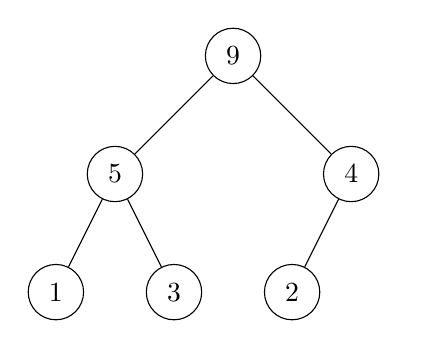
\begin{tikzpicture}[
every node/.style = {minimum width = 2em, draw, circle},
  level/.style = {sibling distance = 30mm/#1}
]
\node {9}
    child {node {5} 
        child {node {1}}
        child {node {3}}
    }
    child {node {4}
        child {node {2}}
        % child {node {75}}
        child {edge from parent[draw = none]}
    };
\end{tikzpicture}
\caption{Max heap}
\end{figure}

\begin{figure}[ht]
\centering
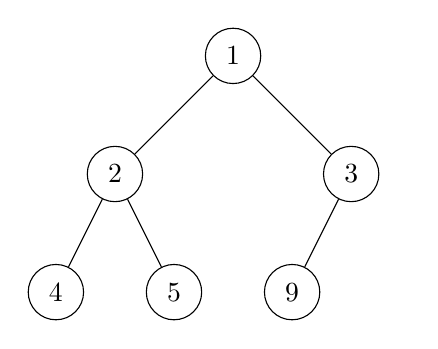
\begin{tikzpicture}[
every node/.style = {minimum width = 2em, draw, circle},
  level/.style = {sibling distance = 30mm/#1}
]
\node {1}
    child {node {2} 
        child {node {4}}
        child {node {5}}
    }
    child {node {3}
        child {node {9}}
        % child {node {75}}
        child {edge from parent[draw = none]}
    };
\end{tikzpicture}
\caption{Min heap}
\end{figure}

\noindent You can implement a tree structure by a pointer or an array. We choose to use the array implementation like below. In terms of space complexity, the array implementation has more benefits than the pointer implementation. In the array representation of a heap, for an element in array index $i$,
\begin{itemize}
    \item The parent node would be at index $\lfloor  \frac{i-1}{2}\rfloor$.
    \item The left child would be at index $2i + 1$.
    \item The right child would be at index $2i + 2$.
    \item The root node will be at index 0
\end{itemize}

\begin{figure}[ht]
	\centering
% 	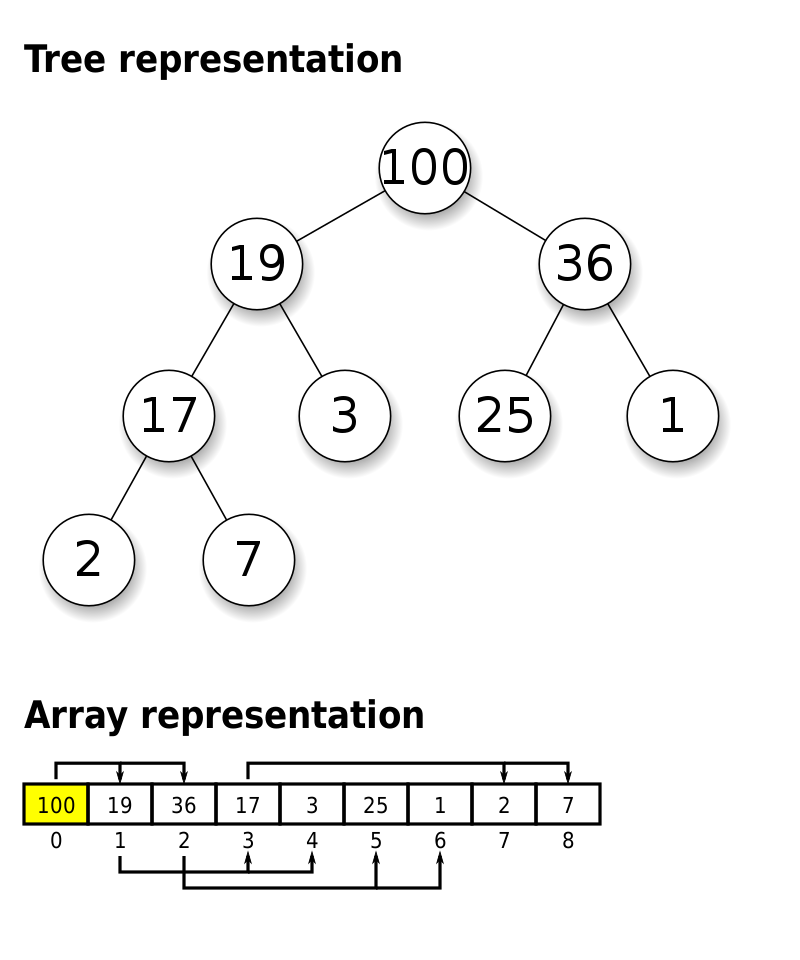
\includegraphics[scale=0.3]{code/sort/pic/heap_rep.png}
    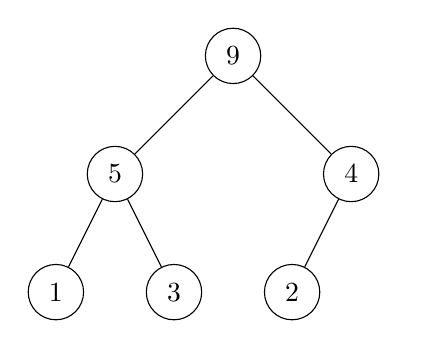
\begin{tikzpicture}[
every node/.style = {minimum width = 2em, draw, circle},
  level/.style = {sibling distance = 30mm/#1}
]
\node (1) {9}
    child {node (2) {5} 
        child {node (3) {1}}
        child {node (4) {3}}
    }
    child {node (5) {4}
        child {node (6) {2}}
        % child {node {75}}
        child {edge from parent[draw = none]}
    };
    % \draw[dashed, ->] (1) to[out=0, in=180] (2);
    % \draw[dashed, ->] (2) to[out=0, in=180] (5);
    % \draw[dashed, ->] (5) to[out=0, in=180] (3);
    % \draw[dashed, ->] (3) to[out=0, in=180] (4);
    % \draw[dashed, ->] (4) to[out=0, in=180] (6);
   
\end{tikzpicture}
	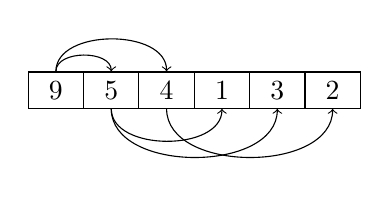
\begin{tikzpicture}[>=to, 
    every node/.style = {minimum width = 2em, draw, rectangle, node distance={2em}},
      level/.style = {sibling distance = 1em/#1}
    ]
    \node (1) {9};
    \node (2) [right of=1] {5};
    \node (3) [right of=2] {4};
    \node (4) [right of=3] {1};
    \node (5) [right of=4] {3};
    \node (6) [right of=5] {2};
    
    \draw[->] (1) to[out=90, in=90] (2);
    \draw[->] (1) to[out=90, in=90] (3);
    \draw[->] (2) to[out=270, in=270] (4);
    \draw[->] (2) to[out=270, in=270] (5);
    \draw[->] (3) to[out=270, in=270] (6);
    \end{tikzpicture}
    \caption{Array representation of heap}
\end{figure}

\begin{figure}[ht]
\centering
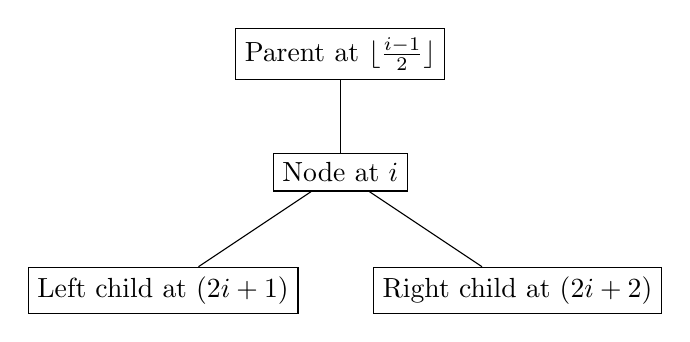
\begin{tikzpicture}[
every node/.style = {minimum width = 4em, draw, rectangle},
  level/.style = {sibling distance = 90mm/#1}
]
\node {Parent at $\lfloor  \frac{i-1}{2}\rfloor$}
    child {node {Node at $i$} 
        child {node {Left child at $(2i + 1)$}}
        child {node {Right child at $(2i + 2)$}}
    };
\end{tikzpicture}
\caption{Heap relationship}
\end{figure}

\textbf{Applications of Heaps}

\begin{enumerate}
    \item \textit{Priority Queues} can be implemented using heaps.
    \item Heap is used in heap sort.
    \item Heaps are used in implementing various graph algorithms like \textit{Dijkstra's algorithm} and \textit{Prim's algorithm}.
    \item If we want to get ordered statistics, heaps serve as a great choice. If we want the kth smallest or largest element, we can pop the heap k times to retrieve them.
\end{enumerate}

\subsection{Heapify}

\noindent The process of creating a heap data structure using the binary tree is called heapify. It is used to create a Max-Heap or a Min-Heap. You need two operations to build a Max-heap (Min-heap) from an arbitrary array.
\begin{enumerate}
    \item \lstinline{heapify}: to make some node and its descendant nodes meet the heap property.
    \item \lstinline{buildHeap}: to produce a heap from an arbitrary array.
\end{enumerate}

\begin{itemize}
    \item  \lstinline{buildHeap}:
\begin{enumerate}
    \item We are given an array. Firstly we will create a complete binary tree from the array.
    \item Start from the first index of non-leaf node whose index is given by \lstinline{n/2 - 1} where \lstinline{n} is the length of the array. We will apply \lstinline{heapify} on this node.
    \item Perform reverse level order traversal from last non-leaf node and \lstinline{heapify} each node. 
\end{enumerate}

\item \lstinline{heapify}: 
\begin{enumerate}
    \item Set current element \lstinline{i} as \lstinline{largest} (\lstinline{smallest}).
    \item The index of left child is given by \lstinline{2i + 1} and the right child is given by \lstinline{2i + 2}.
    \begin{enumerate}
        \item If left child is greater (smaller) than current element (i.e. element at \lstinline{i}th index), set \lstinline{leftChildIndex} as \lstinline{largest} (\lstinline{smallest}).
        \item If right child is greater (smaller) than the element in \lstinline{largest} (\lstinline{smallest}), set \lstinline{rightChildIndex} as \lstinline{largest} (\lstinline{smallest}).
    \end{enumerate}
    \item Swap \lstinline{largest} (\lstinline{smallest}) with current element.
    \item Repeat \lstinline{heapify} to the \lstinline{largest} (\lstinline{smallest}) element recursively.
\end{enumerate}

\end{itemize}

\begin{lstlisting}
'''Max heap implementation'''

def heapify(arr, i):
    # To heapify a subtree rooted with node i which is an index in arr. N is size of heap
    largest = i  # Initialize largest as root
    leftChildIndex = 2*i + 1  # leftChildIndex = 2*i + 1
    rightChildIndex = 2*i + 2  # rightChildIndex = 2*i + 2

    N = len(arr)
 
    # If leftChildIndex child is larger than root
    if leftChildIndex < N and arr[leftChildIndex] > arr[largest]:
        largest = leftChildIndex
 
    # If rightChildIndex child is larger than largest so far
    if rightChildIndex < N and arr[rightChildIndex] > arr[largest]:
        largest = rightChildIndex
 
    # If largest is not root
    if largest != i:
        arr[i], arr[largest] = arr[largest], arr[i]
 
        # Recursively heapify the affected sub-tree
        heapify(arr, largest)
 

def buildHeap(arr):
    # Function to build a Max-Heap from the given array index of last non-leaf node
    N = len(arr)
    startIdx = N // 2 - 1
 
    # Perform reverse level order traversal from last non-leaf node and heapify each node
    for i in range(startIdx, -1, -1):
        heapify(arr, i)
 
if __name__ == '__main__':
    # Binary Tree Representation of input array
    #             1
    #           /    \
    #         3        5
    #       /  \     /  \
    #     4      6  13  10
    #    / \    / \
    #   9   8  15 17
    arr = [1, 3, 5, 4, 6, 13, 10, 9, 8, 15, 17]
 
    buildHeap(arr)
    print(arr)

    # Final Heap:
    #             17
    #           /    \
    #         15      13
    #        /  \     / \
    #       9     6  5   10
    #      / \   / \
    #     4   8 3   1
\end{lstlisting}
\textbf{Output}
\begin{lstlisting}
[17, 15, 13, 9, 6, 5, 10, 4, 8, 3, 1]
\end{lstlisting}

\noindent \textbf{Time complexity}: The function \lstinline{heapify} exchanges two items in an array, which runs in constant time and recursively calls itself. So the time complexity of \lstinline{heapify} will be in proportional to the number of repeats. In the worst case, \lstinline{heapify} should repeat the operation the height of the tree times. This is because in the worst case, \lstinline{heapify} will exchange the root nodes with the most depth leaf node. Therefore the time complexity of \lstinline{heapify} is $O(\log_2 n)$ time. The function \lstinline{buildHeap} basically calls \lstinline{heapify} and makes $O(n)$ such calls. So the overall time complexity is $O(n\log_2 n)$.

\subsection{Percolation: Bubbling up and down}

\noindent When elements are added or removed, the structure must also fulfil the heap property. This may require some items to swap and ``bubble up" to the top of the heap while some other items to ``bubble down" to their rightful position in order to keep the structure of the heap. Percolation take $O(\log_2 n)$ time as it needs to swap elements along the height of the tree.
\vspace{5mm}

\begin{figure}
\centering
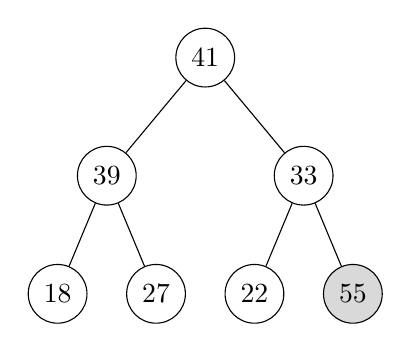
\begin{tikzpicture}[
every node/.style = {minimum width = 2em, draw, circle},
  level/.style = {sibling distance = 25mm/#1}
]
\node {41}
    child {node {39} 
        child {node {18}}
        child {node {27}}
    }
    child {node {33}
        child {node {22}}
        child {node[fill=gray!30] {55}}
    };
\end{tikzpicture}
\hspace{5mm}
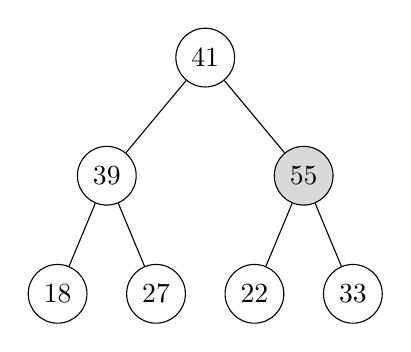
\begin{tikzpicture}[
every node/.style = {minimum width = 2em, draw, circle},
  level/.style = {sibling distance = 25mm/#1}
]
\node {41}
    child {node {39} 
        child {node {18}}
        child {node {27}}
    }
    child {node[fill=gray!30] {55}
        child {node {22}}
        child {node {33}}
    };
\end{tikzpicture}
\vspace{5mm}

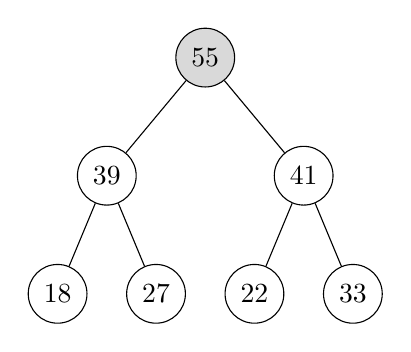
\begin{tikzpicture}[
every node/.style = {minimum width = 2em, draw, circle},
  level/.style = {sibling distance = 25mm/#1}
]
\node[fill=gray!30] {55}
    child {node {39} 
        child {node {18}}
        child {node {27}}
    }
    child {node {41}
        child {node {22}}
        child {node {33}}
    };
\end{tikzpicture}
\caption{Percolation: Bubble up for max-heap}
\label{fig:bubbleup}
\end{figure}

\begin{figure}
    \centering
    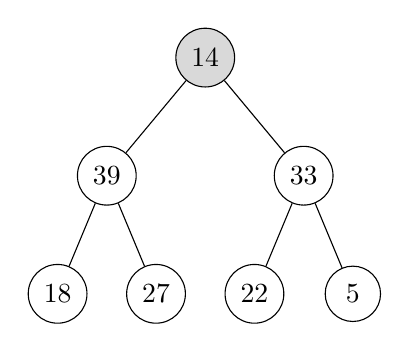
\begin{tikzpicture}[
    every node/.style = {minimum width = 2em, draw, circle},
      level/.style = {sibling distance = 25mm/#1}
    ]
    \node[fill=gray!30] {14}
        child {node {39} 
            child {node {18}}
            child {node {27}}
        }
        child {node {33}
            child {node {22}}
            child {node {5}}
        };
    \end{tikzpicture}
    \hspace{5mm}
    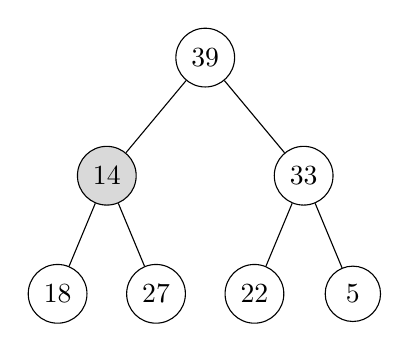
\begin{tikzpicture}[
    every node/.style = {minimum width = 2em, draw, circle},
      level/.style = {sibling distance = 25mm/#1}
    ]
    \node {39}
        child {node[fill=gray!30] {14} 
            child {node {18}}
            child {node {27}}
        }
        child {node {33}
            child {node {22}}
            child {node {5}}
        };
    \end{tikzpicture}
    \vspace{5mm}
    
    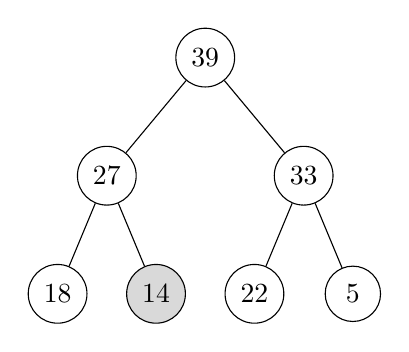
\begin{tikzpicture}[
    every node/.style = {minimum width = 2em, draw, circle},
      level/.style = {sibling distance = 25mm/#1}
    ]
    \node {39}
        child {node {27} 
            child {node {18}}
            child {node[fill=gray!30] {14}}
        }
        child {node {33}
            child {node {22}}
            child {node {5}}
        };
    \end{tikzpicture}
    \caption{Percolation: Bubble down for max-heap}
\label{fig:bubbledown}
\end{figure}
    
\begin{lstlisting}
def bubble_up(arr, i):
# This function will bubble up the element at index i (for max-heap)
    parentIndex = (i-1)//2
    if parentIndex < 0:
        return
    # If the element is grater than the parent element, swap values with the parent
    if arr[i] > arr[parentIndex]:
        arr[i], arr[parentIndex] = arr[parentIndex], arr[i]
        bubble_up(arr, parentIndex)


def bubble_down(arr, i):
    # This function will bubble down the element at index i (for max-heap)
    largest = i  # Initialize largest as root
    leftChildIndex = 2*i + 1  # leftChildIndex = 2*i + 1
    rightChildIndex = 2*i + 2  # rightChildIndex = 2*i + 2

    N = len(arr)
    if leftChildIndex > N:
        return
 
    # If leftChildIndex child is larger than root
    if leftChildIndex < N and arr[leftChildIndex] > arr[largest]:
        largest = leftChildIndex
 
    # If rightChildIndex child is larger than largest so far
    if rightChildIndex < N and arr[rightChildIndex] > arr[largest]:
        largest = rightChildIndex
 
    # If largest is not root
    if largest != i:
        arr[i], arr[largest] = arr[largest], arr[i]
 
        # Recursively heapify the affected sub-tree
        bubble_down(arr, largest)


if __name__ == "__main__":
    arr = [41, 39, 33, 18, 27, 22, 55]
    print('Initial array:', arr)
    bubble_up(arr, 6)
    print('After bubbling up:', arr)
    arr = [14, 39, 33, 18, 27, 22, 5]
    print('Initial array:', arr)
    bubble_down(arr, 0)
    print('After bubbling down:', arr)
    print()
    arr = [17, 15, 2, 13, 9, 6, 5, 10, 4, 8, 16, 3, 1]
    print('Initial array:', arr)
    bubble_up(arr, 10)
    print('After bubbling up:', arr)
    arr = [17, 15, 2, 13, 9, 6, 5, 10, 4, 8, 3, 1]
    print('Initial array:', arr)
    bubble_down(arr, 2)
    print('After bubbling down:', arr)
\end{lstlisting}
\textbf{Output}
\begin{lstlisting}
Initial array: [41, 39, 33, 18, 27, 22, 55]
After bubbling up: [55, 39, 41, 18, 27, 22, 33]
Initial array: [14, 39, 33, 18, 27, 22, 5]
After bubbling down: [39, 27, 33, 18, 14, 22, 5]

Initial array: [17, 15, 2, 13, 9, 6, 5, 10, 4, 8, 16, 3, 1]
After bubbling up: [17, 16, 2, 13, 15, 6, 5, 10, 4, 8, 9, 3, 1]
Initial array: [17, 15, 2, 13, 9, 6, 5, 10, 4, 8, 3, 1]
After bubbling down: [17, 15, 6, 13, 9, 2, 5, 10, 4, 8, 3, 1]
\end{lstlisting}

\subsection{Insert element into heap}
\begin{enumerate}
    \item Insert the new element at the end of the array.
    \item Bubble-up the element through the array.
\end{enumerate}
\noindent Time complexity: $O(\log_2 n)$
\begin{lstlisting}
def insertNode(arr, element):
    arr.append(element)
    N = len(arr)
    bubble_up(arr, N-1)
\end{lstlisting}

\subsection{Delete element from heap}
\begin{enumerate}
    \item Find the index element to be deleted.
    \item Swap it with the last element.
    \item Delete the last element
    \item Bubble-down the element through the array.
\end{enumerate}
\noindent Time complexity: $O(\log_2 n)$
\begin{lstlisting}
def deleteNode(arr, element):
    N = len(arr)
    i = 0 # To find the index of the element to be removed
    for i in range(0, N):
        if element == arr[i]:
            break
    # Swap with the last item
    arr[i], arr[N-1] = arr[N-1], arr[i]
    arr.remove(element)
    bubble_down(arr, i)
\end{lstlisting}

\subsection{Heapsort}

\noindent Heapsort is one kind of sorting algorithm using a heap data structure. Note that the order of sort is ascending for min-heap while the order is descending for max-heap.

\begin{enumerate}
    \item Build a heap from an arbitrary array with \lstinline{buildHeap}.
\end{enumerate}

\subsection{Priority queues}
\noindent A priority queue is a special type of queue in which each element is associated with a priority value. And, elements are served on the basis of their priority. That is, higher priority elements are served first (not first-in-first-out rule). However, if elements with the same priority occur, they are served according to their order in the queue. Generally, the value of the element itself is considered for assigning the priority. We can perform two operations on a priority queue:
\begin{enumerate}
    \item \textbf{add}(element): This function will insert `element' into the priority queue.
    \item \textbf{poll}(): This function will remove the highest priority element from the priority queue. 
\end{enumerate}

\noindent Priority queue can be implemented using an array, a linked list, a heap data structure, or a binary search tree. Among these data structures, heap data structure provides an efficient implementation of priority queues. 
\begin{itemize}
    \item If higher priority corresponds to higher number in the element, then a \textit{max-heap} can be used to implement the priority queue. this is known as \textit{descending order priority queue}.
    
    \item If higher priority corresponds to lower number in the element, then a \textit{min-heap} can be used to implement the priority queue. this is known as \textit{ascending order priority queue}.
\end{itemize}

\noindent Adding an element to a priority queue is equivalent to adding the element into the corresponding heap. The polling element from the priority queue is basically deleting the root node form the heap.

\section{Graph}

\noindent A graph is a common data structure that consists of a finite set of nodes (or vertices) and a set of edges connecting them. Generally, a graph $G$ is represented as $G = (V, E)$, where $V$ is set of vertices and $E$ is set of edges.

\begin{figure}
    \centering
    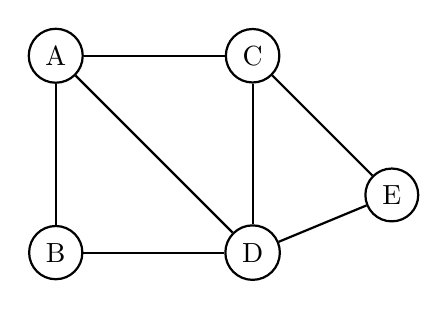
\begin{tikzpicture}[node distance={25mm}, thick, main/.style = {draw, circle}] 
\node[main] (A) {A}; 
\node[main] (B) [below of=A] {B}; 
\node[main] (C) [right of=A] {C}; 
\node[main] (D) [below of=C] {D}; 
\node[main] (E) [below right of=C] {E}; 
\draw[-] (A) -- (B); 
\draw[-] (A) -- (C); 
% \draw (1) to [out=135,in=90,looseness=1.5] (5); 
% \draw (1) to [out=180,in=270,looseness=5] (1); 
\draw (B) -- (D); 
\draw (C) -- (D);
\draw[-] (A) -- (D);
\draw (C) -- (E);
\draw (D) -- (E);
% \draw[->] (5) to [out=315, in=315, looseness=2.5] (3); 
% \draw[->] (6) -- node[midway, above right, sloped, pos=1] {+1} (4); 
\end{tikzpicture} 
    \caption{Graph data structure}
    \label{fig:graph}
\end{figure}

\noindent The figure \ref{fig:graph} is a graph with 5 vertices and 6 edges. This graph can be defined as $G = ( V , E )$ where $$V = \{A,B,C,D,E\}$$ and $$E = \{(A,B),(A,C)(A,D),(B,D),(C,D),(C,E),(D,E)\}$$

\subsection{Directed and Undirected graph}

\noindent A graph can be directed or undirected. In an undirected graph, edges are not associated with the directions with them. An undirected graph is shown in the figure \ref{fig:graph} since its edges are not attached with any of the directions. If an edge exists between vertex $A$ and $B$ then the vertices can be traversed from $B \rightarrow A$ as well as $A \rightarrow B$. In a directed graph, edges form an ordered pair. Edges represent a specific path from some vertex $A$ to another vertex $B$. Node $A$ is called initial node while node $B$ is called terminal node. A directed graph is shown in the figure \ref{fig:graph2}.
\begin{figure}
    \centering
    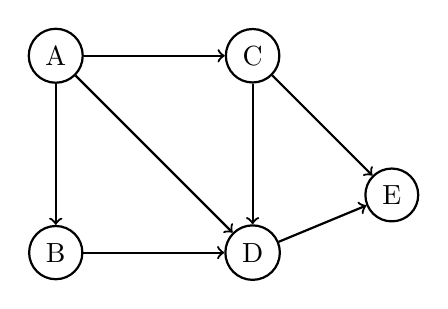
\begin{tikzpicture}[node distance={25mm}, thick, main/.style = {draw, circle}] 
\node[main] (A) {A}; 
\node[main] (B) [below of=A] {B}; 
\node[main] (C) [right of=A] {C}; 
\node[main] (D) [below of=C] {D}; 
\node[main] (E) [below right of=C] {E}; 
\draw[->] (A) -- (B); 
\draw[->] (A) -- (C); 
% \draw (1) to [out=135,in=90,looseness=1.5] (5); 
% \draw (1) to [out=180,in=270,looseness=5] (1); 
\draw[->] (B) -- (D); 
\draw[->] (C) -- (D);
\draw[->] (A) -- (D);
\draw[->] (C) -- (E);
\draw[->] (D) -- (E);
% \draw[->] (5) to [out=315, in=315, looseness=2.5] (3); 
% \draw[->] (6) -- node[midway, above right, sloped, pos=1] {+1} (4); 
\end{tikzpicture} 
    \caption{Directed graph}
    \label{fig:graph2}
\end{figure}
\subsection{Graph terminologies}
\begin{itemize}
    \item \textbf{Path}: A path can be defined as the sequence of nodes that are followed in order to reach some terminal node $v$ from the initial node $u$.

\item \textbf{Closed path}: A path with sequence of nodes $\{v_0, v_1, \cdots v_N\}$ will be called as closed path if the initial node is same as terminal node i.e. a path will be closed path if $v_0=v_N$.

\item \textbf{Simple path}: If all the nodes of the graph are distinct with an exception $v_0=v_N$, then such path $P$ is called as closed simple path.

\item \textbf{Cycle}: A cycle can be defined as the path which has no repeated edges or vertices except the first and last vertices.

\item \textbf{Connected graph}: A connected graph is the one in which some path exists between every two vertices $(u, v)$ in $V$. There are no isolated nodes in connected graph.

\item \textbf{Complete graph}: A complete graph is the one in which every node is connected with all other nodes. A complete graph contain $\frac{n(n-1)}{2}$ edges where $n$ is the number of nodes in the graph.

\item \textbf{Weighted graph}: In a weighted graph, each edge is assigned with some number such as length or weight. The weight of an edge $e$ can be given as $w(e)$ which must be a positive (+) value indicating the cost of traversing the edge.

\item \textbf{Digraph}: A digraph is a directed graph in which each edge of the graph is associated with some direction and the traversing can be done only in the specified direction.

\item \textbf{Loop}: An edge from a vertex to itself.

\item \textbf{Adjacent nodes}: If two nodes $u$ and $v$ are connected via an edge $e$, then the nodes $u$ and $v$ are called as neighbours or adjacent nodes.

\item \textbf{Degree of the node}: A degree of a node is the number of edges that are connected with that node. A node with degree 0 is called an \textit{isolated node}.

\item \textbf{Order}: The number of vertices in the graph.

\item \textbf{Size}: The number of edges in the graph.
\end{itemize}

\subsection{Graph implementations}

\noindent There are three main ways to implement graphs:
\begin{enumerate}
    \item \textbf{Adjacency matrix}
    
    \noindent In adjacency matrix, we represent the graph $G = (V,E)$ in a two-dimensional array of $n \times n$ elements where $n = |V|$ is the number of nodes. If $ij$th element $a_{ij}$ of the matrix is 1, this means that there is an edge connecting vertex $i$ with vertex $j$. 
    \[
    a_{ij}= 
\begin{cases}
    1,& \text{if there is an edge from } i \rightarrow  j\\
    0,              & \text{otherwise}
\end{cases}
\]
    For weighted graph,
    \[
    a_{ij}= 
\begin{cases}
    w_{ij},& \text{if there is an edge from } i \rightarrow  j\\
    0,              & \text{otherwise}
\end{cases}
\]
    This approach if very fast for look-ups. Because we can instantly get the value in the cell $ij$. But it's also very heavy on memory because we have to reserve a space in memory for every possible edge $n \times n$.
    \begin{table}[ht]
    \centering
\begin{tabular}{llllll}
\multicolumn{1}{c}{}   & \multicolumn{1}{c}{A}  & \multicolumn{1}{c}{B}  & C                      & D                      & E                      \\ \cline{2-6} 
\multicolumn{1}{l|}{A} & \multicolumn{1}{l|}{0} & \multicolumn{1}{l|}{1} & \multicolumn{1}{l|}{1} & \multicolumn{1}{l|}{1} & \multicolumn{1}{l|}{0} \\ \cline{2-6} 
\multicolumn{1}{l|}{B} & \multicolumn{1}{l|}{1} & \multicolumn{1}{l|}{0} & \multicolumn{1}{l|}{0} & \multicolumn{1}{l|}{1} & \multicolumn{1}{l|}{0} \\ \cline{2-6} 
\multicolumn{1}{l|}{C} & \multicolumn{1}{l|}{1} & \multicolumn{1}{l|}{0} & \multicolumn{1}{l|}{0} & \multicolumn{1}{l|}{1} & \multicolumn{1}{l|}{1} \\ \cline{2-6} 
\multicolumn{1}{l|}{D} & \multicolumn{1}{l|}{1} & \multicolumn{1}{l|}{1} & \multicolumn{1}{l|}{1} & \multicolumn{1}{l|}{0} & \multicolumn{1}{l|}{0} \\ \cline{2-6} 
\multicolumn{1}{l|}{E} & \multicolumn{1}{l|}{0} & \multicolumn{1}{l|}{0} & \multicolumn{1}{l|}{1} & \multicolumn{1}{l|}{1} & \multicolumn{1}{l|}{0} \\ \cline{2-6} 
\end{tabular}
\caption{Adjacency matrix for figure \ref{fig:graph}}
\end{table}
    \item \textbf{Adjacency lists}
    
    \noindent In adjacency lists, an array of lists is used to represent the graph. The size of the array is equal to the number of vertices. An entry $\text{array}[i]$ represents the list of vertices adjacent to the $i$th vertex. This representation can also be used to represent a weighted graph. The weights of edges can be represented as lists of pairs. The adjacency matrix for figure \ref{fig:graph} is given in the following:
    \begin{lstlisting}
    A ---> B ---> C ---> D ---> Null
    B ---> A ---> D ---> Null
    C ---> A ---> D ---> E ---> Null
    D ---> A ---> B ---> C ---> E ---> Null
    E ---> C ---> D ---> Null
    \end{lstlisting}
    \item \textbf{Adjacency sets}
    
    \noindent This is a new alternative to adjacency lists. Instead of having an array of linked lists, have it be an array of sets. An entry $\text{array}[i]$ represents the set of vertices adjacent to the $i$th vertex. The adjacency matrix for figure \ref{fig:graph} is given in the following:
    \begin{lstlisting}
    [
        {A, B, C, D}, 
        {B, A, D}, 
        {C, A, D, E}, 
        {D, A, B, C, E}, 
        {E, C, D}
    ]
    \end{lstlisting}
\end{enumerate}

\noindent If $m$ is the number of neighbors of a given vertex, and $v$ is the number of vertices in the graph, then the time complexity comparison for different representations are given in the following table.
\begin{table}[ht]
\centering 
\begin{tabular}{lccc}
\textbf{Operation}                             & \textbf{\begin{tabular}[c]{@{}c@{}}Adjacency \\ Matrix\end{tabular}} & \textbf{\begin{tabular}[c]{@{}c@{}}Adjacency \\ List\end{tabular}} & \textbf{\begin{tabular}[c]{@{}c@{}}Adjacency \\ Sets\end{tabular}} \\ \cline{2-4} 
\multicolumn{1}{l|}{Edge existence check}      & \multicolumn{1}{c|}{$O(1)$}                                          & \multicolumn{1}{c|}{$O(m)$}                                        & \multicolumn{1}{c|}{$O(1)$}                                        \\ \cline{2-4} 
\multicolumn{1}{l|}{Iterating over neighbours} & \multicolumn{1}{c|}{$O(|V|)$}                                          & \multicolumn{1}{c|}{$O(m)$}                                        & \multicolumn{1}{c|}{$O(m)$}                                        \\ \cline{2-4} 
\multicolumn{1}{l|}{Adding an edge}            & \multicolumn{1}{c|}{$O(1)$}                                          & \multicolumn{1}{c|}{$O(1)$}                                        & \multicolumn{1}{c|}{$O(1)$}                                        \\ \cline{2-4} 
\multicolumn{1}{l|}{Removing an edge}          & \multicolumn{1}{c|}{$O(1)$}                                          & \multicolumn{1}{c|}{$O(m)$}                                        & \multicolumn{1}{c|}{$O(1)$}                                        \\ \cline{2-4} 
\end{tabular}
\caption{Time complexity comparison}
\end{table}

\subsection{Depth First Search (DFS)}

\noindent DFS (Depth-first search) is technique used for traversing a tree or graph. Here backtracking is used for traversal. In this traversal first the farthest node along the path is visited and then backtracks to the previous node. A standard DFS implementation puts each vertex of the graph into `visited' category. The purpose of the algorithm is to mark each vertex as visited while avoiding cycles. The DFS algorithm works as follows:
\begin{enumerate}
    \item Start by putting any one of the graph's vertices on top of a stack.
    \item Take the top item of the stack and add it to the visited list.
    \item Create a list of that vertex's adjacent nodes. Add the ones which aren't in the visited list to the top of the stack.
    \item Keep repeating steps 2 and 3 until the stack is empty.
\end{enumerate}

\begin{figure}
    \centering
    \begin{tikzpicture}[
    every node/.style = {minimum width = 2em, draw, circle, node distance={15mm}},
      level/.style = {sibling distance = 30mm/#1}
    ]
    \node (0) {0};
    \node (1) [right of=1] {1};
    \node (2) [below of=0] {2};
    \node (3) [right of=1] {3}; 
    \node (4) [right of=2] {4};
    \node (5) [right of=4] {5};
    \node (6) [right of=3] {6};
    \node (7) [right of=5] {7};
    \node (8) [above of=3] {8};
    \node (9) [right of=8] {9};
    \draw[-] (0) -- (1);
    \draw[-] (1) -- (3);
    \draw[-] (3) -- (6);
    \draw[-] (0) -- (2);
    \draw[-] (1) -- (4);
    \draw[-] (2) -- (4);
    \draw[-] (4) -- (5);
    \draw[-] (5) -- (7);
    \draw[-] (3) -- (8);
    \draw[-] (8) -- (9);
    \end{tikzpicture}
    \caption{Graph for the given DFS python program}
    \label{fig:graph_program}
\end{figure}

\begin{lstlisting}
# Iterative approach using a stack
def dfs_iterative(graph, node):            
    visited = set()
    # Create a stack for DFS
    stack = []
    # Push the current node.
    stack.append(node)

    while len(stack) != 0:
        # Pop a vertex from stack
        node = stack.pop()

        # Stack may contain same vertex twice. So we need to print the popped item only if it is not visited and add the item in the visited list
        if node not in visited:
            print(node, end=' ')
            visited.add(node)
            
        # Get all adjacent vertices of the popped vertex. If a adjacent has not been visited, then push it to the stack.
        for neighbour in graph[node] - visited:
            if neighbour not in visited:
                stack.append(neighbour)

# Recursive approach
def dfs_recursive(graph, node, visited = set()):
    if node in visited:
        return
    else:
        print(node, end=" ")
        visited.add(node)
        for neighbour in graph[node] - visited:
            dfs_recursive(graph, neighbour, visited)


if __name__ == "__main__":
    graph = {
        '0': set(['1', '2']),
        '1': set(['0', '3', '4']),
        '2': set(['0', '4']),
        '3': set(['1', '6', '8']),
        '4': set(['1', '2', '5']),
        '5': set(['4', '7']),
        '6': set(['3']),
        '7': set(['5']),
        '8': set(['3', '9']),
        '9': set(['8'])
    }
    print("Iterative approach")
    dfs_iterative(graph, '0')
    print()
    print("Recursive approach")
    dfs_recursive(graph, '0')
\end{lstlisting}
\textbf{Output}
\begin{lstlisting}
Iterative approach
0 1 4 2 5 7 3 6 8 9 
Recursive approach
0 2 4 5 7 1 3 8 9 6
\end{lstlisting}

\noindent Time complexity: $O(|V| + |E|)$\\
\noindent Space Complexity: $O(|V|)$ for the \lstinline{visited} array

\subsubsection{Applications}

\begin{enumerate}
    \item Used to find a path between two vertices.
\item Used to detect cycles in a graph.
\item Used in topological sorting.
\end{enumerate}

\subsection{Breadth First Search (BFS)}

\noindent Breadth-first search (BFS) is a graph traversal algorithm that starts traversing from any node and explores all the neighbouring nodes before moving to the neighbour of neighbours. Similar to DFS, the standard BFS implementation puts each vertex of the graph into `visited' category. The purpose of the algorithm is to mark each vertex as visited while avoiding cycles. The BFS algorithm works as follows:

\begin{enumerate}
\item  Start by putting any one of the graph’s vertices at the back of a queue.
\item Take the front item of the queue and add it to the visited list.
\item Create a list of that vertex's adjacent nodes. Add those which are not within the visited list to the rear of the queue.
\item Keep repeating steps 2 and 3 until the queue is empty.
\end{enumerate}


\begin{figure}
    \centering
     \begin{tikzpicture}[
    every node/.style = {minimum width = 2em, draw, circle, node distance={15mm}},
      level/.style = {sibling distance = 30mm/#1}
    ]
    \node (0) {0};
    \node (1) [right of=1] {1};
    \node (2) [below of=0] {2};
    \node (3) [right of=1] {3}; 
    \node (4) [right of=2] {4};
    \node (5) [right of=4] {5};
    \node (6) [right of=3] {6};
    \node (7) [right of=5] {7};
    \node (8) [above of=3] {8};
    \node (9) [right of=8] {9};
    \draw[-] (0) -- (1);
    \draw[-] (1) -- (3);
    \draw[-] (3) -- (6);
    \draw[-] (0) -- (2);
    \draw[-] (1) -- (4);
    \draw[-] (2) -- (4);
    \draw[-] (4) -- (5);
    \draw[-] (5) -- (7);
    \draw[-] (3) -- (8);
    \draw[-] (8) -- (9);
    \end{tikzpicture}
    \caption{Graph for the given BFS python program}
    \label{fig:graph_program_bfs}
\end{figure}

\begin{lstlisting}
# Iterative approach using a queue
def bfs_iterative(graph, node):
    visited = set()
    # Create a queue for BFS
    queue = []
    # Push the current node.
    queue.insert(0, node)

    while len(queue) != 0:
        # Pop a vertex from queue
        node = queue.pop()

        # queue may contain same vertex twice. So we need to print the popped item only if it is not visited and add the item in the visited list
        if node not in visited:
            print(node, end=' ')
            visited.add(node)
            
        # Get all adjacent vertices of the popped vertex. If a adjacent has not been visited, then push it to the stack.
        for neighbour in graph[node] - visited:
            if neighbour not in visited:
                queue.insert(0, neighbour)
                
                
if __name__ == "__main__":
    graph = {
        '0': set(['1', '2']),
        '1': set(['0', '3', '4']),
        '2': set(['0', '4']),
        '3': set(['1', '6', '8']),
        '4': set(['1', '2', '5']),
        '5': set(['4', '7']),
        '6': set(['3']),
        '7': set(['5']),
        '8': set(['3', '9']),
        '9': set(['8'])
    }
    print("Iterative approach")
    bfs_iterative(graph, '0')
\end{lstlisting}
\textbf{Output}
\begin{lstlisting}
Iterative approach
0 1 2 3 4 6 8 5 9 7
\end{lstlisting}
\noindent Time complexity: $O(|V| + |E|)$\\
\noindent Space Complexity: $O(|V|)$ for the \lstinline{visited} array

\subsubsection{Applications}

\begin{enumerate}
    \item Used to determine the shortest path and \textbf{minimum spanning tree}.
\item Used by search engine crawlers to build indexes of web pages.
\item Used to search on social networks.
\item Used to find available neighbour nodes in peer-to-peer networks such as BitTorrent.
\end{enumerate}

\subsection{Shortest path}

\noindent The shortest path from one vertex to another vertex is a path in the graph such that the sum of the weights of the edges that should be travelled is minimum.

\subsubsection{Dijkstra's Algorithm}

\begin{enumerate}
    \item Create a list of ``distances'' $d$ equal to the number of nodes $n$ and initialize each value to infinity.
    $$d[v] = \infty, \hspace{5mm}\forall v = 0,1,2,\cdots (n-1)$$
    \item Set the ``distances'' to the starting node equal to 0 since the distance from the source node to itself is 0. If $v_0$ is the index of the starting node, then
    $$d[v_0] = 0$$
    \item Create a list of ``visited'' nodes $u$ set to False for each node (since we haven't visited any yet).
    $$u[v] = \text{False}, \hspace{5mm}\forall v = 0,1,2,\cdots (n-1)$$
    \item Loop through $n$ iterations:
    \begin{enumerate}
        \item Select the node with index $v$ for which the distance $d[v]$ is minimum and $u[v] = \text{False}$.
        \item Set that node to visited i.e. $u[v] = \text{True}$.
        \item Perform \textbf{relaxation} to all its adjacent nodes. If $\sigma$ is the index of an adjacent node, then update the distance $d[\sigma]$ as follows:
        $$d[\sigma] = \min\left(d[\sigma], d[v] + l(v,\sigma)\right)$$
        where $l(v,\sigma)$ is the length corresponding to the edge between the nodes at index $v$ and $\sigma$.
    \end{enumerate}
    \item The original ``distances'' list should now contain the shortest distance to each node or infinity if a node is unreachable from the desired starting node.
\end{enumerate}
\noindent N.B. This algorithm requires that there are no negative weight edges in the graph.
\vspace{5mm}

\tikzstyle{vertex}=[draw=black,shape=circle,fill=white!20, edge=black,minimum size=20pt,inner sep=0pt]
\tikzstyle{edge} = [draw,thick,-]
\tikzstyle{arrow} =[draw,thick,->]
\tikzstyle{weight} = [font=\scriptsize]
\noindent \textbf{Example of Dijkstra's algorithm}:
\begin{figure}[ht]
\centering
\begin{tikzpicture}[scale=2,auto,swap]
    \foreach \pos /\name in {{(0,0)}/1,{(1,1)}/3,{(0,2)}/2,{(2,2)}/4,{(2,1)}/5}
        \node[vertex](\name) at \pos{$\name$};
    \foreach \source /\dest /\weight in {1/5/2,2/1/5,3/5/3,4/2/8,5/2/7,5/4/5} 
        \path[edge] (\source) -- node[weight] {$\weight$} (\dest);
    \foreach \source /\dest /\weight/\pos in {1/3/1/{above left}, 3/2/2/{below left}} 
        \path[edge] (\source) -- node[weight, \pos] {$\weight$} (\dest);
\end{tikzpicture}
\caption{Example graph for Dijkstra's algorithm}
\end{figure}

\begin{table}[H]
\centering
\begin{tabular}{|c|c|c|}
\hline
\multicolumn{1}{|l|}{\textbf{Vertex}} & \textbf{distances  $d$} & \textbf{visited $u$} \\ \hline
1   & 0             & False     \\ 
2   & $\infty$      & False     \\ 
3   & $\infty$      & False     \\ 
4   & $\infty$      & False     \\ 
5   & $\infty$      & False     \\ \hline
\end{tabular}
\caption{Dijkstra's algorithm: Initial step}
\end{table}

\begin{table}[H]
\centering
\begin{tabular}{|c|r|c|}
\hline
\multicolumn{1}{|l|}{\textbf{Vertex}} & \textbf{distances  $d$} & \textbf{visited $u$} \\ \hline
1*   & 0             & True     \\ 
2   & $\min(\infty, 0+5)=5$      & False     \\ 
3   & $\min(\infty, 0+1)=1$      & False     \\ 
4   &  $\infty$     & False     \\ 
5   & $\min(\infty, 0+2)=2$      & False     \\ \hline
\end{tabular}
\caption{Dijkstra's algorithm: After 1st iteration}
\end{table}

\begin{table}[H]
\centering
\begin{tabular}{|c|r|c|}
\hline
\multicolumn{1}{|l|}{\textbf{Vertex}} & \textbf{distances  $d$} & \textbf{visited $u$} \\ \hline
1   & 0             & True     \\ 
2   & $\min(5, 1+2)=3$      & False     \\ 
3*   & 1      & True     \\ 
4   &  $\infty$     & False     \\ 
5   & $\min(2, 1+3)=2$      & False     \\ \hline
\end{tabular}
\caption{Dijkstra's algorithm: After 2nd iteration}
\end{table}

\begin{table}[H]
\centering
\begin{tabular}{|c|r|c|}
\hline
\multicolumn{1}{|l|}{\textbf{Vertex}} & \textbf{distances  $d$} & \textbf{visited $u$} \\ \hline
1   & 0             & True     \\ 
2   & $\min(3, 2+7) = 3$      & False     \\ 
3   & $\min(1, 2+2) = 1$      & True     \\ 
4   & $\min(\infty, 2+5) = 7$      & False     \\ 
5*   & 2      & True     \\ \hline
\end{tabular}
\caption{Dijkstra's algorithm: After 3rd iteration}
\end{table}

\begin{table}[H]
\centering
\begin{tabular}{|c|r|c|}
\hline
\multicolumn{1}{|l|}{\textbf{Vertex}} & \textbf{distances  $d$} & \textbf{visited $u$} \\ \hline
1   & 0             & True     \\ 
2*   & 3      & True     \\ 
3   & 1      & True     \\ 
4   & $\min(7, 3+8)= 7$      & False     \\ 
5   & $\min(2, 3+3)= 2$      & True     \\ \hline
\end{tabular}
\caption{Dijkstra's algorithm: After 4th iteration}
\end{table}

\begin{table}[H]
\centering
\begin{tabular}{|c|c|c|}
\hline
\multicolumn{1}{|l|}{\textbf{Vertex}} & \textbf{distances  $d$} & \textbf{visited $u$} \\ \hline
1   & 0             & True     \\ 
2   & 3      & True     \\ 
3   & 1      & True     \\ 
4*   & 7      & True     \\ 
5   & 2      & True     \\ \hline
\end{tabular}
\caption{Dijkstra's algorithm: After 5th iteration}
\end{table}

\begin{lstlisting}
def dijkstras(graph, starting_node):
    n = len(graph)
    
    # Step 1: Initialize distance list (dict) as all infinities
    distances = {x: float("Inf") for x in graph.keys()}
    
    # Step 2: Set the distance for the starting_node to be 0
    distances[starting_node] = 0
    
    # Step 3: Initialize list (dict) of visited nodes
    visited = {x: False for x in graph.keys()}
    
    # Step 4: Loop through n iterations
    for _ in range(n):
        
        # Step 4a: Select the node for which the distance is minimum and is not visited before.
        u = -1
        for i in graph.keys():
            if not visited[i] and (u == -1 or distances[i] < distances[u]):
                u = i
        # All the nodes have been visited or we can't reach this node
        if distances[u] == float("Inf"):
            break
        
        # Step 4b: Set the node as visited
        visited[u] = True
        
        # Step 4c: Performing relaxation to all adjacent nodes
        for v, l in graph[u]:
            if distances[u] + l < distances[v]:
                distances[v] = distances[u] + l
    return distances


if __name__ == "__main__":
    # Create our graph using an adjacency list representation
    # each "node" in our list should be a node index and a distance
    graph = {
        '0': [('1', 1)],
        '1': [('0', 1), ('2', 2), ('3', 3)],
        '2': [('1', 2), ('3', 1), ('4', 5)],
        '3': [('1', 3), ('2', 1), ('4', 1)],
        '4': [('2', 5), ('3', 1)]
    }
    print(dijkstras(graph, '1'))
\end{lstlisting}
\textbf{Output}
\begin{lstlisting}
{'0': 1, '1': 0, '2': 2, '3': 3, '4': 4}
\end{lstlisting}
\subsubsection{Time complexity}
\noindent We have a loop with $n=|V|$ iterations. On each iteration, we need to find the minimum distance node. Then we need to update the distance of all the adjacent node. In the worst case this operation will take $O(|V|)$ time. Thus overall we have the time complexity $O(|V|^2)$. The space complexity is $O(|V|)$, since we have to maintain two lists $d$ and $u$ each of length $|V|$.

\subsubsection{Bellman-Ford algorithm}
% \subsubsection{Floyd-Warshall algorithm}

\subsection{Minimum spanning tree (MST)}

\noindent A \textit{spanning tree} is a sub-graph of an undirected connected graph, which includes all the vertices of the graph with a minimum possible number of edges. If a vertex is missed, then it is not a spanning tree. The edges may or may not have weights assigned to them. 

\noindent A \textit{minimum spanning tree} (MST) is a spanning tree in which the sum of the weight of the edges is the minimum.

\subsubsection{Kruskal's algorithm}

\noindent It falls under a class of algorithms called greedy algorithms that find the local optimum in the hopes of finding a global optimum. We start from the edges with the lowest weight and keep adding edges until we reach our goal. The steps for implementing Kruskal's algorithm are as follows:
\begin{enumerate}
    \item Sort all the edges from low weight to high.
    \item Take the edge with the lowest weight and add it to the spanning tree. If adding the edge created a cycle, then reject this edge.
    \item Keep adding edges until we reach all vertices.
\end{enumerate}

\begin{lstlisting}
# https://www.techiedelight.com/kruskals-algorithm-for-finding-minimum-spanning-tree/
# A class to represent a disjoint set
class DisjointSet:
    parent = {}
 
    # perform MakeSet operation
    def makeSet(self, n):
        # create `n` disjoint sets (one for each vertex)
        for i in range(n):
            self.parent[i] = i
 
    # Find the root of the set in which element `k` belongs
    def find(self, k):
        # if `k` is root
        if self.parent[k] == k:
            return k
 
        # recur for the parent until we find the root
        return self.find(self.parent[k])
 
    # Perform Union of two subsets
    def union(self, a, b):
        # find the root of the sets in which elements `x` and `y` belongs
        x = self.find(a)
        y = self.find(b)
 
        self.parent[x] = y
 
 
# Function to construct MST using Kruskal's algorithm
def runKruskalAlgorithm(edges, n):
 
    # stores the edges present in MST
    MST = []
 
    # Initialize `DisjointSet` class.
    # Create a singleton set for each element of the universe.
    ds = DisjointSet()
    ds.makeSet(n)
 
    index = 0
 
    # sort edges by increasing weight
    edges.sort(key=lambda x: x[2])
 
    # MST contains exactly `V-1` edges
    while len(MST) != n - 1:
 
        # consider the next edge with minimum weight from the graph
        (src, dest, weight) = edges[index]
        index = index + 1
 
        # find the root of the sets to which two endpoints
        # vertices of the next edge belongs
        x = ds.find(src)
        y = ds.find(dest)
 
        # if both endpoints have different parents, they belong to
        # different connected components and can be included in MST
        if x != y:
            MST.append((src, dest, weight))
            ds.union(x, y)
 
    return MST
 
 
if __name__ == '__main__':
    # (u, v, w) triplet represent undirected edge from
    # vertex `u` to vertex `v` having weight `w`
    edges = [
        (0, 1, 7), (1, 2, 8), (0, 3, 5), (1, 3, 9), (1, 4, 7), (2, 4, 5),
        (3, 4, 15), (3, 5, 6), (4, 5, 8), (4, 6, 9), (5, 6, 11)
    ]
 
    # total number of nodes in the graph (labelled from 0 to 6)
    n = 7
 
    # construct graph
    e = runKruskalAlgorithm(edges, n)
 
    print(e)
\end{lstlisting}
\textbf{Output}
\begin{lstlisting}
[(0, 3, 5), (2, 4, 5), (3, 5, 6), (0, 1, 7), (1, 4, 7), (4, 6, 9)]
\end{lstlisting}

\subsubsection{Prim's algorithm}

\noindent Like Kruskal's algorithm, Prim's algorithm is also a Greedy algorithm. It starts with an empty spanning tree.
\begin{enumerate}
    \item At first the spanning tree consists only of a single vertex (chosen arbitrarily). 
    \item Then the minimum weight edge outgoing from this vertex is selected and added to the spanning tree. After that the spanning tree already consists of two vertices. 
    \item Now select and add the edge with the minimum weight that has one end in an already selected vertex (i.e. a vertex that is already part of the spanning tree), and the other end in an unselected vertex. 
    \item The process is repeated until the spanning tree contains all vertices.
\end{enumerate}

\begin{figure}[ht]
	\centering
	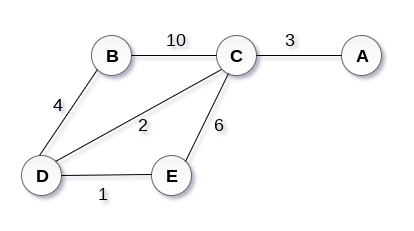
\includegraphics[scale=0.45]{code/sort/pic/prim1.png}
	\caption{Prim's algorithm: starting graph}
	\label{fig:prim1}
\end{figure}

\noindent As an example, lets construct a minimum spanning tree of the graph given in the figure \ref{fig:prim1} by using Prim's algorithm.

\begin{figure}[ht]
	\centering
	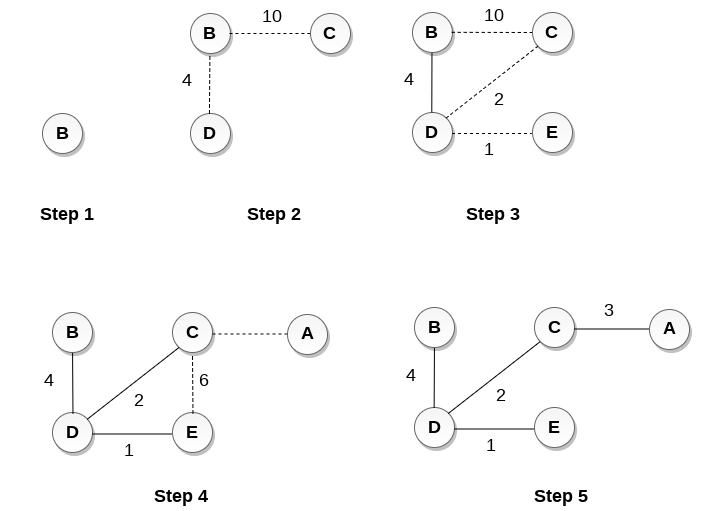
\includegraphics[scale=0.45]{code/sort/pic/prim2.png}
	\caption{Prim's algorithm steps}
\end{figure}

\begin{itemize}
    \item Choose a starting vertex $B$.
\item Find the vertices that are adjacent to $B$. The edges that connecting the vertices are shown by dotted lines.
\item Choose the edge with the minimum weight among all. i.e. $BD$ and add it to MST. Now find all the edges that are adjacent to $B$ or $D$ and which are not yet selected i.e. $BC$, $CD$ and $DE$.
\item Choose the edge with the minimum weight among all. In this case, the edge $CD$ is chosen. Add them to MST and then explore the edges adjacent to $B$, $C$ and $D$ i.e. $CE$ and $AC$.
\item Choose the edge with the minimum weight i.e. $AC$. (We can't choose $CE$ as it would cause cycle in the graph.)

\end{itemize}
\noindent The graph produces in the final step is the minimum spanning tree of the graph shown in the above figure. The cost of MST is calculated as 4 + 2 + 1 + 3 = 10 units.

\begin{lstlisting}
def prim_algo(G):
    # Number of vertices in graph
    V = len(G)

    # Create a array to track selected vertex
    # Selected will become True otherwise False
    selected = [False]*V
    # Initially set number of edge to 0
    num_edge = 0
    # Choose 0th vertex and make it true
    selected[0] = True
    # Print for edge and weight
    print("Edge : Weight")
    while (num_edge < V-1):
        # For every vertex in 'selected', find the all adjacent vertices
        # Calculate the distance from the vertex selected at step 1.
        # If the vertex is already in 'selected', discard it
        # Choose another vertex nearest to selected vertex  at step 1.
        minimum = float("inf") # To store the minimum edge
        x = 0 # To store the vertex from 'selected' when the edge toward 'not selected' is minimum
        y = 0 # To store the vertex not from 'selected' when the edge toward 'selected' is minimum
        for i in range(V):
            if selected[i]:
                for j in range(V):
                    if ((not selected[j]) and G[i][j] > 0):  
                        # Not in selected and there is an edge
                        if minimum > G[i][j]:
                            minimum = G[i][j]
                            x = i
                            y = j
        print(str(x) + "-" + str(y) + " : " + str(G[x][y]))
        selected[y] = True
        num_edge += 1


if __name__ == "__main__":
    # Adjacency matrix representation of a graph
    G = [[0, 9, 75, 0, 0],
        [9, 0, 95, 19, 42],
        [75, 95, 0, 51, 66],
        [0, 19, 51, 0, 31],
        [0, 42, 66, 31, 0]]

    prim_algo(G)
\end{lstlisting}
\textbf{Output}
\begin{lstlisting}
Edge : Weight
0-1 : 9
1-3 : 19
3-4 : 31
3-2 : 51
\end{lstlisting}

\noindent Time complexity: At every iteration of the loop, we add one node to the tree. Since there are $|V|$ nodes, it follows that there are $O(|V|)$ iterations of this loop. Within each iteration of the loop, we need to find and test edges in the tree. If there are $|E|$ edges, the naive searching implementation uses $O(|E|)$ to find the edge with minimum weight. So in combination, we should expect the complexity to be $O(|V||E|)$, which may be $O(|V|^3)$ in the worst case.\\
Space complexity: $O(|V|)$

\section{Disjoint sets}

\newpage
\chapter{Algorithm Techniques}

\section{Brute force approach}

\section{Divide and conquer method}

\noindent Divide and conquer is an algorithm design paradigm. A divide-and-conquer algorithm recursively breaks down a problem into two or more sub-problems of the same or related type, until these become simple enough to be solved directly. Here are the steps involved:
\begin{enumerate}
    \item \textbf{Divide}: Divide the given problem into sub-problems using recursion.
    \item \textbf{Conquer}: Solve the smaller sub-problems recursively. If the subproblem is small enough, then solve it directly.
    \item \textbf{Combine}: Combine the solutions of the sub-problems that are part of the recursive process to solve the actual problem.
\end{enumerate}
% \noindent This approach saves us a lot of space, but it's slower than adjacency matrix.
\subsection{Binary search}

\textbf{Given a sorted array \lstinline{arr} of $n$ elements, write a function to search a given element $x$ in \lstinline{arr}.}
\vspace{4mm}

\noindent Binary search algorithm:
\begin{enumerate}
    \item Compare $x$ with the middle element.
    \item If $x$ matches with the middle element, we return the mid index.
    \item Else If $x$ is greater than the mid element, then $x$ can only lie in the right half subarray after the mid element. So we call the algorithm on the right half recursively.
    \item Else ($x$ is smaller) call the algorithm on the left half recursively.
\end{enumerate}
\vspace{5mm}

\noindent Time complexity: $O(\log n)$\\
\noindent Space complexity: $O(1)$

\begin{lstlisting}
def binarySearch(arr, left, right, element):
    # Check base case
    if right >= left:
        mid = left + (right - left) // 2
        # If element is present at the middle itself
        if arr[mid] == element:
            return mid
        # If element is smaller than mid, then it can only be present in left subarray
        elif arr[mid] > element:
            return binarySearch(arr, left, mid-1, element)
        # Else the element can only be present in right subarray
        else:
            return binarySearch(arr, mid + 1, right, element)
    else:
        # Element is not present in the array
        return -1
  
  
if __name__ == "__main__":
    arr = [2, 3, 4, 10, 40]
    element = 10
    result = binarySearch(arr, 0, len(arr)-1, element)
    
    if result != -1:
        print("Element is present at index % d" % result)
    else:
        print("Element is not present in array")
\end{lstlisting}
\textbf{Output}
\begin{lstlisting}
Element is present at index  3
\end{lstlisting}

\section{Greedy approach}

\noindent A \textbf{greedy algorithm}, as the name suggests, always makes the choice that seems to be the best at that moment. This means that it makes a locally-optimal choice in the hope that this choice will lead to a globally-optimal solution.

\noindent Assume that you have an objective function that needs to be optimized (either maximized or minimized) at a given point. A Greedy algorithm makes greedy choices at each step to ensure that the objective function is optimized. The Greedy algorithm has only one shot to compute the optimal solution so that it never goes back and reverses the decision. Greedy algorithms have some advantages and disadvantages:
\begin{itemize}
    \item It is quite easy to come up with a greedy algorithm (or even multiple greedy algorithms) for a problem.
    \item Analyzing the run time for greedy algorithms will generally be much easier than for other techniques (like Divide and conquer).
    \item The difficult part is that for greedy algorithms you have to work much harder to understand correctness issues. Even with the correct algorithm, it is hard to prove why it is correct.
\end{itemize}

\subsection{Coin change problem}

\noindent \textbf{Given a value $n$ and an infinite supply of coins with denominations 1, 5, 10 and 20 each, find the list coins to make the change so that the number of coins is minimum.}
\vspace{5mm}

\noindent Let's start by having the values of the coins in an array in reverse sorted order i.e., \lstinline{denominations = [20, 10, 5, 1]}.

\noindent Now if we have to make a value of $n$ using these coins, then we will check for the first element in the array (greedy choice) and if it is greater than $n$, we will move to the next element, otherwise take it. Now after taking one coin with value \lstinline{denominations[i]}, the total value which we have to make will now become \lstinline{n-denominations[i]}.

\begin{lstlisting}
def coin_change_greedy(n):
    denominations = [20, 10, 5, 1]
    i = 0
    min_coins = []

    while(n > 0):
        if denominations[i] > n:
            i += 1
        else:
            min_coins.append(denominations[i])
            n = n - denominations[i]
    return min_coins

if __name__ == '__main__':
    print(coin_change_greedy(23))
\end{lstlisting}
\textbf{Output}
\begin{lstlisting}
[20, 1, 1, 1]
\end{lstlisting}
\noindent We can easily see that the algorithm is not going to take more than linear time. As $n$ is decreased by \lstinline{denominations[i]} at the end of the while loop, we can say that for most of the cases it will take much less than $O(n)$ time. So, we can say that our algorithm has $O(n)$ time complexity.

\subsection{Job sequencing problem with deadlines}

\noindent \textbf{Given a list of tasks with deadlines and total profit earned on completing a task, find the maximum profit earned by executing a list of tasks within a maximum specified deadline. Assume that each task takes one unit of time to complete, and a task can't execute beyond its deadline. Also, only a single task will be executed at a time.}

\vspace{5mm}

\noindent Example:
\begin{lstlisting}
Input:  Five Jobs with following deadlines and profits
JobID   Deadline  Profit
  a       2        100
  b       1        19
  c       2        27
  d       1        25
  e       3        15
Maximum deadline: 10
Output: Following is maximum profit sequence of jobs
        c, a, e
\end{lstlisting}

\noindent A simple solution is to generate all subsets of given set of jobs and check individual subset for feasibility of jobs in that subset. Keep track of maximum profit among all feasible subsets. The time complexity of this solution is exponential. We can also solve this problem using greedy method which is more optimal than simple solution. So let's solve this problem via greedy method. 
To solve the job sequencing problem via greedy method follow this steps:

\begin{enumerate}
    \item Sort all jobs in decreasing order of profit.
    \item Iterate through the jobs and perform the following:
    \begin{enumerate}
        \item Choose a slot $i$ if $i<\text{deadline}$ for the job and $i$ is maximum.
        \item If no such slot exists, ignore the job and continue.
    \end{enumerate}
    \item Do following for remaining $n-1$ jobs.
    \item If the current job can fit in the current result sequence without missing the deadline, add current job to the result. Else ignore the current job.
\end{enumerate}

\begin{figure}[ht]
	\centering
	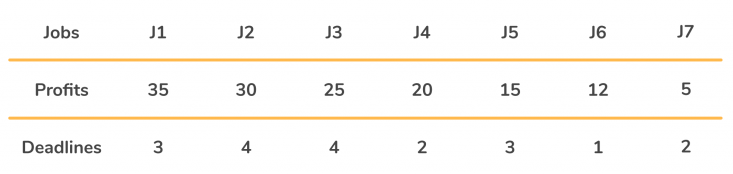
\includegraphics[scale=0.35]{code/sort/pic/job1.png}
\end{figure}

\begin{figure}[ht]
	\centering
	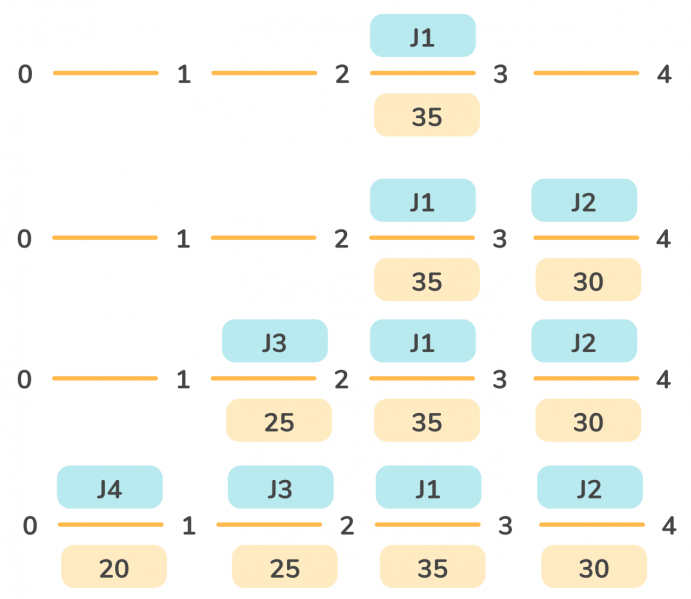
\includegraphics[scale=0.35]{code/sort/pic/job2.png}
\end{figure}

\noindent Time complexity $O(n^2)$.
\begin{lstlisting}
# A class to store job details. Each job has an identifier,
# a deadline, and profit associated with it.
class Job:
    def __init__(self, taskId, deadline, profit):
        self.taskId = taskId
        self.deadline = deadline
        self.profit = profit
 
 
# Function to schedule jobs to maximize profit
def scheduleJobs(jobs, T):
 
    # stores the maximum profit that can be earned by scheduling jobs
    profit = 0
 
    # list to store used and unused slots info
    slot = [-1] * T
 
    # arrange the jobs in decreasing order of their profits
    jobs.sort(key=lambda x: x.profit, reverse=True)
 
    # consider each job in decreasing order of their profits
    for job in jobs:
        # search for the next free slot and map the task to that slot
        for j in reversed(range(job.deadline)):
        # for j in range(job.deadline):
            if j < T and slot[j] == -1:
                slot[j] = job.taskId
                profit += job.profit
                break
 
    # print the scheduled jobs
    print('The scheduled jobs are', list(filter(lambda x: x != -1, slot)))
 
    # print total profit that can be earned
    print('The total profit earned is', profit)
 
 
if __name__ == '__main__':
 
    # List of given jobs. Each job has an identifier, a deadline, and
    # profit associated with it
    jobs = [
        Job('T1', 9, 15), 
        Job('T2', 2, 2), 
        Job('T3', 5, 18), 
        Job('T4', 7, 1), 
        Job('T5', 4, 25),
        Job('T6', 2, 20), 
        Job('T7', 5, 8), 
        Job('T8', 7, 10), 
        Job('T9', 4, 12), 
        Job('T10', 3, 5)
    ]
 
    # Maximum deadline
    T = 15
 
    # schedule jobs and calculate the maximum profit
    scheduleJobs(jobs, T)
\end{lstlisting}
\textbf{Output}
\begin{lstlisting}
The scheduled jobs are ['T7', 'T6', 'T9', 'T5', 'T3', 'T4', 'T8', 'T1']
The total profit earned is 109
\end{lstlisting}

\section{Fractional knapsack problem}

\section{Backtracking method}

\noindent Backtracking is an improvement of the \textit{brute-force approach}. It tries to search for a solution to a problem among all the available options. It finds a solution set by developing a solution step by step, increasing levels with time, using recursive calling. Since a problem would have constraints, the solutions that fail to satisfy them will be removed. In order to find these solutions, a search tree named \textbf{state-space tree} is used. In a state-space tree, each branch is a variable, and each level represents a solution.
\vspace{4mm}
% \noindent A backtracking algorithm uses the \textit{depth-first search} method. When it starts exploring the solutions, the algorithm checks if the so-far built solution satisfies the constraints. If it does, it continues searching. If it doesn't, the branch would be eliminated, and the algorithm goes back to the level before. 

\noindent Before start solving the problem we must be able to recognize if it can be solved using a backtracking algorithm. There are the following types of problems that can be solved using backtracking:
\begin{enumerate}
    \item \textbf{Decision Problem}: In this type of problem we always search for a feasible solution.
    \item \textbf{Optimization Problem}: In this type of problem we always search for the best possible solution.
    \item \textbf{Enumeration Problem}: In this type of problem we try to find all feasible solutions.
\end{enumerate}
\subsection{Suitcase password problem}

\textbf{Consider a suitcase lock, where a three-digit password is forgotten. Assume the digits are restricted to binary number and the unknown password is said to be having at most one 0. Construct a backtracking solution to generate all possible passwords.}

\begin{figure}[ht]
    \centering
    \begin{tikzpicture}[
every node/.style = {minimum width = 2em, draw, circle},
  level/.style = {sibling distance = 65mm/#1}
]
\node {Root}
    child {node[fill=green!20] {1} 
        child {node[fill=green!20] {11}
            child {node[fill=green!20] {111} edge from parent node[left,draw=none] {1}}
            child {node[fill=green!20] {110} edge from parent node[right,draw=none] {0}}
        edge from parent node[left,draw=none] {1} }
        child {node[fill=green!20] {10}
            child {node[fill=green!20] {101} edge from parent node[left,draw=none] {1}}
            child {node[fill=red!35] {100} edge from parent node[right,draw=none] {0}}
        edge from parent node[right,draw=none] {0}}
    edge from parent node[left,draw=none] {1}}
    child {node[fill=green!20] {0}
        child {node[fill=green!20] {01}
            child {node[fill=green!20] {011} edge from parent node[left, draw=none] {1}}
            child {node[fill=red!35] {010} edge from parent node[right,draw=none] {0}}
        edge from parent node[left,draw=none] {1}}
        child {node[fill=red!35] {00}
            child {node[fill=red!35] {001} edge from parent node[left,draw=none] {1}}
            child {node[fill=red!35] {000} edge from parent node[right,draw=none] {0}}
        edge from parent node[right,draw=none] {0}}
    edge from parent node[right,draw=none] {0}};
\end{tikzpicture}
    \caption{Suitcase password problem}
    \label{fig:suitcase}
\end{figure}

\noindent The potential password is of three digits which can be visualized as three digits $(x_1, x_2, x_3)$ where $x_i \in \{0,1\}, i = 1,2,3$. To construct a state-space tree, start with a Root. There are two choices 1 or 0, at every stage. This leads to the generation of the binary tree as shown in the figure \ref{fig:suitcase}. It can be observed all potential passwords are marked with green while all non-relevant passwords are marked with red. Check all the green leaves of the tree to find the valid solution.

\begin{lstlisting}
password_list = []

# Recursive helper function, adds character until length is reached
def add_character(arr, i, s, N):
    # Base case
    if (i == 0): # when len has been reached
        # print out the elements of the state-space tree
        print(s)
        if len(s) == N:
            password_list.append(s)
        return
     
    # Iterate through the array
    for j in arr:
        # 1. Create new string after appending next character 
        # 2. In case there is already one zero we will not append any zero
        # 3. Call add_character() again until string has reached its length
        if j == '0' and s.count('0') == 1:
            # Solution is not feasible, so skip
            continue
        
        appended = s + j
        add_character(arr, i-1, appended, N)
 
    return
 
# Function to generate all possible passwords
def generate(arr, N):
    # arr: Array of characters used in the password
    # N: Length of the password
    for i in range(1, N+1):
        add_character(arr, i, "", N)

     
if __name__ == "__main__":
    arr = ['1', '0'] # Array of characters used in the password
    N = 3  # Length of the password
    print('The elements of the state-space tree:')
    generate(arr, N)
    print('password_list:', password_list)
\end{lstlisting}
\textbf{Output}
\begin{lstlisting}
The elements of the state-space tree:
1
0
11
10
01
111
110
101
011
password_list: ['111', '110', '101', '011']
\end{lstlisting}

\subsection{Permutation of a string}

\textbf{Given a string $S$, print all the possible permutations of $S$.}
\vspace{5mm}

\noindent A permutation is a rearrangement of the elements of an ordered list $S$ into a one-to-one correspondence with $S$ itself. A string of length $n$ has $n!$ permutation. We will apply backtracking approach to find all the possible solutions by exploring all possible ways. If one of the found solutions turns out to not satisfy the given criteria, it discards the solution and makes some changes and backtracks again.

\begin{lstlisting}
Input: S = "abc"
Output: ["abc", "acb", "bac", "bca", "cba", "cab"]
\end{lstlisting}

\begin{enumerate}
\item Define a pointer \lstinline{idx} which will initially point to the first index of the given string $S$.
\item Now with another pointer $i$ loop through the characters of the string from \lstinline{idx} $\rightarrow$ last charater of the string at $(n-1)$, where $n$ is the length of the string and do the following:
\begin{enumerate}
    \item Swap $S[i]$ and $S[idx]$.
    \item Recall the backtracking function again after moving \lstinline{idx} pointer to the right by one character i.e. \lstinline{idx = idx+1}.
\item When \lstinline{idx} moves to the final character, print the string. This will serve as the base case.
\end{enumerate}
\end{enumerate}

\noindent For example let's take the string \lstinline{"ABC"}. We set the pointer \lstinline{idx} at 0, pointing at the first character \lstinline{"A"}. Swapping \lstinline{"A"} with all the three characters yield \lstinline{"ABC", "BAC", "CBA"}. Now we apply the permutation function again on each of the three strings with \lstinline{idx} pointer set at 1 thereby making the first character fixed. From \lstinline{"ABC"}, we thus get \lstinline{"ABC"} and \lstinline{"ACB"} where \lstinline{"A"} is fixed. Similarly from \lstinline{"BAC"}, we get \lstinline{"BAC"} and \lstinline{"BCA"} and from \lstinline{"CAB"}, we thus get \lstinline{"CAB"} and \lstinline{"CBA"}. After that the \lstinline{idx} pointer set at 2 which is the stopping condition. We then take print out of the six permutations we got so far.
\begin{figure}[ht]
	\centering
	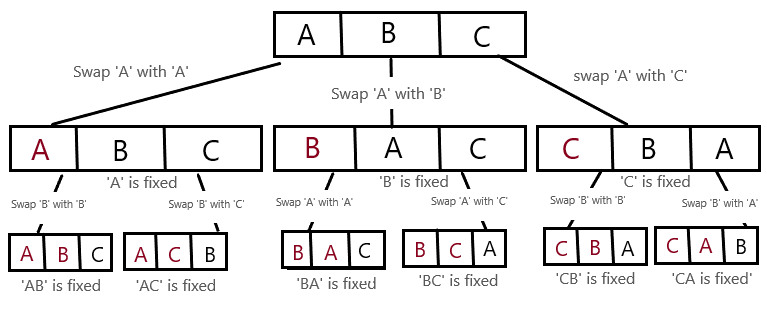
\includegraphics[scale=0.45]{code/sort/pic/recursiontreeabc.png}
\end{figure}
\vspace{5mm}

\noindent Time Complexity: $O(n * n!)$, where $n$ is the length of the string since there are $n!$ permutations and it requires $O(n)$ time to print a permutation.\\
Space Complexity: $O(n!)$, since one has to keep $n!$ solutions.

\begin{lstlisting}
def permutations(char_list, idx=0):
    # Final case
    if idx == len(char_list)-1:
        print(''.join(char_list))
 
    for i in range(idx, len(char_list)):
        # Swap the current index with i
        char_list[idx], char_list[i] = char_list[i], char_list[idx]
        permutations(char_list, idx + 1)
 
if __name__ == '__main__':
    a_string = 'ABC'
    # 'str' object does not support item assignment or swapping, so we convert it to character list
    char_list = [x for x in a_string]
    permutations(char_list)
\end{lstlisting}
\textbf{Output}
\begin{lstlisting}
ABC
ACB
CAB
CBA
ABC
ACB
\end{lstlisting}


\chapter{Sorting Algorithms}

\section{Bubble sort}

\begin{enumerate}
	\item Compare the first two elements of the list to check them which one is greater.
	\item For ascending ordering, place the larger value on the right.
	\item Do the same for second, third elements and so on till the whole list is completed. This is the first round.
	\item Execute steps (1), (2) and (3) for $n$ number of times where $n$ is the length of the list. (In second round you don't need to consider the last element. In third round no need to consider the last two elements and so on.)
\end{enumerate}

\noindent Time complexity: $O(n^2)$ for number of rounds ($n$) $\times$ number of comparisons ($n$) in the worst case

\noindent Space complexity: $O(1)$

\begin{table}[ht]
	\label{Bubble sort}
	\caption{\textbf{Bubble sort: Total round = length(list) - 1 = 3}}
	\vspace{2mm}
	\centering
	\begin{tabular}{cccc}
		&{First round}  &{Second round}  &{Third round}   \\
		&\underline{7} \underline{2} 5 4  &\underline{2} \underline{5} 4 7&\underline{2} \underline{4} 5 7\\
		
		&2 \underline{7} \underline{5} 4&2 \underline{5} \underline{4} 7  &2 4 5 7   \\
		&2 5 \underline{7} \underline{4}  &2 4 5 7 &   \\
		&2 5 4 7  & &\\
		&Iteration num. = 3 &Iteration num. = 2 &Iteration num. = 1 
	\end{tabular}
\end{table}

% \lstinputlisting[language=Python]{code/sort/bubblesort2.py}
\begin{lstlisting}
def bubble_sort(input_list):
	L = len(input_list)
	Round_num = L-1

	for rnd in range(Round_num):
		Iterations_per_round = L - rnd
		for iteration in range(Iterations_per_round):
			for i in range(0, L-1-iteration):
				if input_list[i] > input_list[i+1]:
					swap_value_by_index(input_list, i, i+1)

def swap_value_by_index(a_list, a, b):
    a_list[b], a_list[a] = a_list[a], a_list[b]
\end{lstlisting}
% \textbf{Output:}
% \begin{lstlisting}
% Before sorting:
% [54, 26, 93, 17, 77, 31, 44, 55, 20]
% After bubble sort:
% [17, 20, 26, 31, 44, 54, 55, 77, 93]
% \end{lstlisting}

\newpage
\section{Selection sort}

\begin{enumerate}
	\item The first element is compared with all other elements in the list one-by-one.
	\item If any element is found to be greater than any other element, then they are swapped.
	\item After the first iteration, the smallest number is placed at the first position. The same procedure is repeated for the second element and so on.
\end{enumerate}

\noindent Time complexity: $O(n^2)$

\noindent Space complexity: $O(1)$

\begin{table}[h]
	\label{Selection sort}
	\caption{\textbf{Selection sort: Total round = length(list) - 1 = 3}}
	\vspace{2mm}
	\centering
	\begin{tabular}{cccc}
		&{First round}  &{Second round}  &{Third round}   \\
		&\underline{7} \underline{2} 5 4  &2 \underline{7} \underline{5} 4 &2 4 \underline{7} \underline{5}   \\
		&\underline{2} 7 \underline{5} 4 &2 \underline{5} 7 \underline{4}  &2 4 5 7   \\
		&\underline{2} 7 5 \underline{4}  &2 4 7 5 &   \\
		&2 7 5 4  & &\\
		&Iteration num. = 3 &Iteration num. = 2 &Iteration num. = 1 
	\end{tabular}
\end{table}

\begin{lstlisting}
def selection_sort(input_list):

    L = len(input_list)
    
    # Iteration for 1st element
    for i in range(L-1): 
        # Iteration for 2nd element
        for j in range(i+1, L): 
            min_idx = i # Indicating the min value index
            if input_list[min_idx] > input_list[j]:
                min_idx = j
                swap_value_by_index(input_list, min_idx, i)
                
def swap_value_by_index(a_list, a, b):
    a_list[b], a_list[a] = a_list[a], a_list[b]
\end{lstlisting}
% \textbf{Output:}
% \begin{lstlisting}
% Before sorting:
% [54, 26, 93, 17, 77, 31, 44, 55, 20]
% After selection sort:
% [17, 20, 26, 31, 44, 54, 55, 77, 93]
% \end{lstlisting}

\newpage
\section{Insertion sort}

\begin{enumerate}
	\item The first iteration starts with comparing the first and second elements and ordering them accordingly.
	\item In second iteration, the third element is compared with the first and second elements and placed in a suitable position by shifting other elements.
	\item The procedure is repeated for all elements in the array.
\end{enumerate}

\noindent Time complexity: $O(n^2)$

\noindent Space complexity: $O(1)$

\begin{figure}[ht]
	\centering
	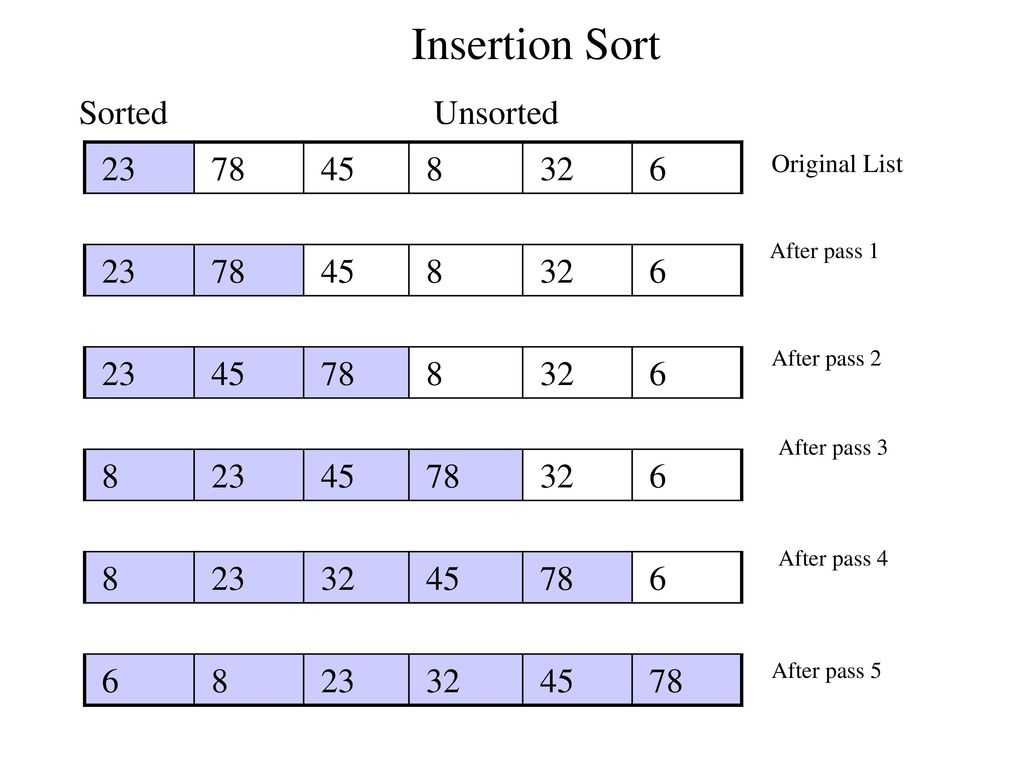
\includegraphics[scale=1.2]{code/sort/pic/picinsertion.jpg}
\end{figure}

\newpage
\begin{lstlisting}
def insertion_sort(input_list):
    L = len(input_list)
    
    for i in range(1, L):
        current_value = input_list[i] # The value currently being compared
        pos = i # Saving the index i in a temporary variable
        
        # Move elements of array [0, 1, 2, ..., (i-1)] that are 
        # greater than current_value to one position ahead of 
        # their current position
        while pos > 0 and input_list[pos - 1] > current_value:
            input_list[pos] = input_list[pos - 1]
            pos -= 1
        # Place the current_value to the gap that is created 
        # after moving the elements that are greater than 
        # current_value to the right.
        input_list[pos] = current_value

if __name__ == "__main__": 
    input_list = [54, 26, 93, 17, 77, 31, 44, 55, 20]
    print("Before sorting:")
    print(input_list)
    insertion_sort(input_list)
    print("After insertion sort:")
    print(input_list)
\end{lstlisting}
\textbf{Output}
\begin{lstlisting}
Before sorting:
[54, 26, 93, 17, 77, 31, 44, 55, 20]
After insertion sort:
[17, 20, 26, 31, 44, 54, 55, 77, 93]
\end{lstlisting}

\newpage
\section{Quick sort}

\noindent Quick sort is a divide-and-conquer algorithm which works by obtaining a \textit{pivot} item from the array and partitioning the array so that all elements smaller than pivot will be on the left side of the array and all elements greater than pivot will be on the right side of the array. The pivot element will be at its final sorted position. Perform the same operation for the sub-arrays on the left and right of pivot.
\begin{enumerate}
    \item Find the pivot item in the array. For simplicity take the first value.
    \item Start a \textit{low} pointer at the second item of the array and a \textit{high} pointer at the last item of the array.
    \item Move the low pointer to the right as long as the element $\leq$ pivot.
    \item Move the high pointer to the left as long as the element $\geq$ pivot.
    \item At this point we find a low pointer value which is higher than the high pointer value. Swap the values only if the low pointer $\leq$ high pointer.
    \item Continue moving the low and high pointer in the same fashion until low pointer crosses the high pointer.
    \item When the low pointer crosses the high pointer, swap the pivot and high pointer value. All the elements to the left of new pivot is smaller than the pivot and all the elements to the right of new pivot is larger than the pivot i.e. the new pivot is in the correct position.
    \item Now we recursively apply the same logic to the left and right sub-array.
\end{enumerate}

\begin{figure}[ht]
	\centering
	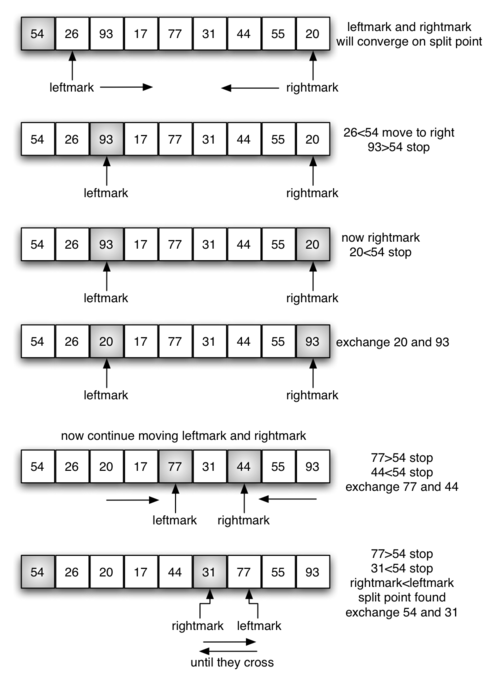
\includegraphics[scale=1.2]{code/sort/pic/partitionA.png}
\end{figure}

\begin{figure}[ht]
	\centering
	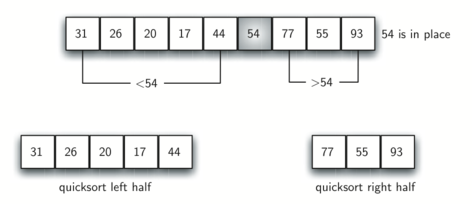
\includegraphics[scale=1.2]{code/sort/pic/partitionB.png}
\end{figure}

\begin{lstlisting}
# This function takes first element as pivot, places the pivot element at its correct position in sorted arr, and places all smaller (smaller than pivot) to left of pivot and all greater elements to right of pivot 
def partition(arr, start, end):
    pivot = arr[start]
    low = start + 1
    high = end
    while True:
        # If the current value we're looking at is less than the pivot, then it's in the right place (right side of pivot) and we can move right, to the next element. 
        # We also need to make sure we haven't surpassed the low pointer, since that indicates we have already moved all the elements to their correct side of the pivot
        while low <= high and arr[low] <= pivot:
            low = low + 1
        
        while low <= high and arr[high] >= pivot:
            high = high - 1

        # We either found a value for both high and low that is out of order or low is higher than high, in which case we exit the loop
        if low <= high:
            arr[low], arr[high] = arr[high], arr[low]
            # The loop continues
        else:
            # We exit out of the loop
            break
    # Swap the pivot and high indexed element
    arr[start], arr[high] = arr[high], arr[start]
    return high


def quick_sort(arr, start, end):
    if start >= end:
        return
    p = partition(arr, start, end)
    quick_sort(arr, start, p-1)
    quick_sort(arr, p+1, end)


if __name__ == "__main__":
    arr = [29, 99, 27, 41, 66, 28, 44]
    print('Before sorting:', arr)
    quick_sort(arr, 0, len(arr) - 1)
    print('After sorting:', arr)
\end{lstlisting}
\textbf{Output}
\begin{lstlisting}
Before sorting: [29, 99, 27, 41, 66, 28, 44]
After sorting: [27, 28, 29, 41, 44, 66, 99]
\end{lstlisting}

\noindent To analyze the \lstinline{quick_sort} function, note that for a list of length $n$, if the partition always occurs in the middle of the list, there will again be $\log n$ divisions. In order to find the split point, each of the $n$ items needs to be checked against the pivot value. The result is $n\log n$. This results in an average case complexity $\Theta(n\log n)$.

\noindent Unfortunately, in the worst case, the split points may not be in the middle and can be very skewed to the left or the right, leaving a very uneven division. In this case, sorting a list of $n$ items divides into sorting a list of 0 items and a list of $n-1$ items. Then sorting a list of $n-1$ divides into a list of size 0 and a list of size $n-2$, and so on. The result is the worst case complexity $O(n^2)$ sort with all of the overhead that recursion requires.

\newpage

\section{Merge sort}

\noindent Merge sort is based on divide-and-conquer approach. It divides the input array into two halves. Each half is solved individually, and then the two sorted halves are merged to get final result.

\vspace{5mm}

\noindent \textbf{MergeSort(array)}
\vspace{3mm}

\noindent If length of array > 1, do the following:
\begin{enumerate}
    \item Find the middle point $m$ 
    $$m = (\text{length of array})/2$$
    \item Divides the input array into two halves
          $$\text{leftArray = array[1:m]}$$
          $$\text{rightArray = array[m:]}$$
    \item Call MergeSort() on both subarray
        $$\text{MergerSort(leftArray)}$$
        $$\text{MergerSort(rightArray)}$$
    \item Merge the two halves sorted in (2) and (3)
        $$ \text{Merge(leftArray, rightArray)}$$
\end{enumerate}

\begin{figure}[ht]
	\centering
	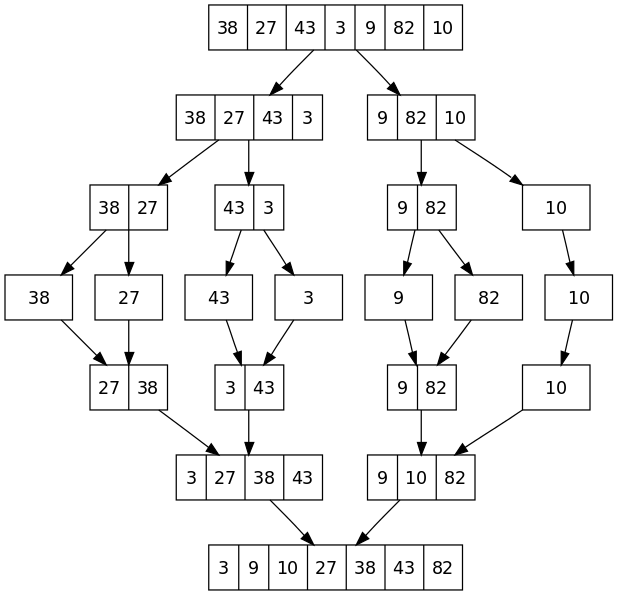
\includegraphics[scale=0.5]{code/sort/pic/mergesort.png}
\end{figure}

\begin{lstlisting}
import math

# This function merge the two sorted subarrays into one single sorted array
def merge(left_array, right_array):
    result = []
    # Left and right index initialized to zero
    L, R = 0, 0
    # Move the two pointer through the two arrays. Append the element to the resultant array whichever is less.
    while (L < len(left_array)) and (R < len(right_array)):
        if left_array[L] < right_array[R]:
            result.append(left_array[L])
            L += 1
        else:
            result.append(right_array[R])
            R += 1
            
    # Remaining part of the subarrays
    left_remains = left_array[L:]
    right_remains = right_array[R:]

    # Concatenate the remaining to the resultant array
    return result + left_remains + right_remains


def merge_sort(arr):
    if len(arr) < 2:
        return arr
    m = math.ceil(len(arr)/2)
    left_array = arr[:m]
    right_array = arr[m:]

    return merge(merge_sort(left_array), merge_sort(right_array))


if __name__ == "__main__":
    arr = [29, 99, 27, 41, 66, 28, 44]
    print('Before sorting:', arr)
    arr = merge_sort(arr)
    print('After sorting:', arr)
\end{lstlisting}
\textbf{Output}
\begin{lstlisting}
Before sorting: [29, 99, 27, 41, 66, 28, 44]
After sorting: [27, 28, 29, 41, 44, 66, 99]
\end{lstlisting}

\newpage

\chapter{Dynamic Programming}

\noindent Dynamic Programming is an algorithmic paradigm that solves a given problem by breaking it into subproblems and save the result  of subproblems for the future so that we will not have to compute that same problem again. Following are the two main properties of a problem that suggests that the given problem can be solved using dynamic programming.

\begin{enumerate}
    \item \textbf{Overlapping subproblems}: Like divide-and-conquer, dynamic programming divide problems into subproblems. In divide-and-conquer strategy, the subproblems are independent of each other; however in dynamic programming, the same subproblems are needed again and again. In dynamic programming, the computed solutions to subproblems are stored in a table so that these don't have to be recomputed. This is called overlapping subproblems.
    \item \textbf{Optimal substructure}: A given problems has optimal substructure property if optimal solution of the given problem can be obtained by using optimal solutions of its subproblems.
\end{enumerate}

\begin{table}[ht]
\centering
\begin{tabular}{p{3.3cm}|p{3.5cm}|p{4.7cm}}
\hline
\multicolumn{1}{c|}{\textbf{Greedy}}                               & \multicolumn{1}{|c|}{\textbf{Divide \& Conquer}}                                                                                 & \multicolumn{1}{|c}{\textbf{Dynamic Programming}}                                                                                    \\ \hline
Optimises by making the best choice at the moment.    & Optimises by breaking down a subproblem into simpler versions of itself and using multi-threading and recursion to solve. & Same as Divide and Conquer, but optimises further by caching the answers to each subproblem as not to repeat the calculation twice. \\ \hline
Doesn't always find the optimal solution, but is very fast. & Always finds the optimal solution, but is slower than Greedy.                                                            & Always finds the optimal solution, but could be pointless on small datasets.                                                \\ \hline 
Requires almost no memory.                                  & Requires some memory to remember recursive calls.                                                                        & Requires a lot of memory for memoisation/tabulation.                                                                       \\ \hline
\end{tabular}
\caption{Difference between Greedy, Divide and Conquer and Dynamic Programming}
\end{table}

\noindent There are two ways dynamic programming can be applied:

\begin{enumerate}
    \item \textbf{Top-down (Memoization) approach}: Top-down breaks the large problem into multiple subproblems. If the subproblem has already been solved, then just reuse the answer. Otherwise, solve the subproblem and store the result. Top-down uses recursion with memoization to avoid recomputing the same subproblem again.
    \item \textbf{Down-top (Tabulation) approach}: Start computing result for the lowest possible subproblem (base) and keep it in a table. Use the subproblem result to solve other subproblems and subsequently keep the results in the table and thus finally solve the whole main problem.
\end{enumerate}

\section{Fibonacci sequence}

\noindent Let's start with a basic example of the \textit{Fibonacci sequence}. Fibonacci sequence is a sequence of positive integers in which the first two elements are 0 and 1 and each of the following elements is the sum of the two preceding ones.

\begin{align*}
    F_0 &= 0,\\
    F_1 &= 1,\\
    F_n &= F_{n-1} + F_{n-2}
\end{align*}

\noindent First solution: Using ordinary \textbf{recursion method}.
\begin{lstlisting}
def fib(n):
    if n <= 1:
       return n
   else:
       return fib(n-1) + fib(n-2)
\end{lstlisting}

\noindent Here, the program will call itself, again and again, to calculate further values as shown in the figure. The calculation of the time complexity of the recursion based approach is around $O(2^n)$. The space complexity of this approach is $O(n)$ as recursion can go max to $n$. In this method values like $F_2$ and $F_3$ are computed multiple times. Imagine the number of repetitions if you have to calculate for $F_{100}$. This method is ineffective for large values.

\begin{center}
    \begin{tikzpicture}[
every node/.style = {minimum width = 1.5em, draw = none, circle},
  level/.style = {sibling distance = 63mm/#1}
]
\node {$F_5$}
    child {node {$F_3$} 
        child {node {$F_1$}}
        child {node {$F_2$}
            child { node {$F_0$}}
            child { node {$F_1$}}
        }
    }
    child {node {$F_4$}
        child {node {$F_2$}
            child { node {$F_0$}}
            child { node {$F_1$}}
        }
        child {node {$F_3$}
            child { node {$F_1$}}
            child {node {$F_2$}
                child { node {$F_0$}}
                child { node {$F_1$}}
            }
        }
        % child {edge from parent[draw = none]}
    };
\end{tikzpicture}
\end{center}

\noindent Second solution: Using \textbf{Top-down method}

\begin{lstlisting}
def fib(n, cache = {}):
    if cache.get(n) != None:
        return cache[n]
    if n <= 1:
        return n
    else:
        res = fib(n-1, cache) + fib(n-2, cache)
        cache[n] = res
        return res
\end{lstlisting}

\noindent Here, the computation time is reduced significantly as the outputs produced after each recursion are stored in a cache which can be reused later. This method is much more efficient than the previous one. Let's now calculate its time complexity.

$$T(n) = T(n-1) + T(n-2) + c$$

\noindent Now when we calculate \lstinline{fib(n-1)}, we already have \lstinline{fib(n-2)} in cache. So the operation \lstinline{fib(n-2)} is 1 (i.e. reading from the cache). Therefore

\begin{align*}
    T(n) &= T(n-1) + 1 + c\\
         &=\left[T(n-2) + 1 + c\right] + 1 + c\\
         &=T(n-2) + 2(1+c)\\
         &= \cdots\\
         &= T(n-k) + k(1+c)
\end{align*}

\noindent Now let's find the value of $k$ for which $n-k = 0$ i.e. $k=n$. Therefore,
\begin{align*}
	T(n) &= T(0) + n(1+c)\\
	     &= 1 + n(1+c) \in O(n)
\end{align*}

\noindent The space complexity is $O(n)$ to store the cache.
\vspace{3mm}

\noindent Third solution: Using \textbf{Bottom-up method}

\begin{lstlisting}
def fib(n):
    if n <= 1:
        return n
    dp = [0]*(n+1)
    dp[0] = 0
    dp[1] = 1 
    for i in range(2, n+1):
        dp[i] = dp[i-1] + dp[i-2]
    return dp[n]
\end{lstlisting}

\noindent This code doesn't use recursion at all. Here, we create an empty list of length $(n+1)$ and set the base case of \lstinline{fib(0)} and \lstinline{fib(1)} at index positions 0 and 1. Then using a for loop for index values 2 up to $n$, the rest of the values are populated in the list. Unlike in the recursive method, the time complexity of this code is linear i.e., it runs in $O(n)$. The space complexity is $O(n)$ because of the requirement of storing the list.

\section{Integers from a given list to add up to a number}

\noindent \textbf{Given a number $n$. Find the number of ways of expressing $n$ as a sum from a list of integers 1, 3, and 4.}
\vspace{5mm}

\noindent If $n = 5$, then there are 6 ways to express $n$ namely, $$\{4,1\}, \{1,4\}, \{1,3,1\}, \{3,1,1\}, \{1,1,3\}, \{1,1,1,1,1\}$$

\noindent Divide the problem into sub-problems for solving it. Let $dp[n]$ be the be the number of ways to write $n$ as the sum of 1, 3, and 4. Consider one possible solution with $n = x_1 + x_2 + x_3 + \cdots + x_k$. If the last number is 1, then sum of the remaining numbers is $n-1$. So the number that ends with 1 will contribute to $dp[n-1]$ number of ways. Similarly the number that ends with 3 and 4 will contribute to $dp[n-3]$ and $dp[n-4]$ number of ways respectively. The final recurrence would be: 

$$dp[n] = dp[n-1] + dp[n-3] + dp[n-4]$$

\noindent with base cases:

$$dp[0] = dp[1] = dp[2] = 1 \text{ and } dp[3] = 2$$

\noindent First solution: Using Top-down approach

\noindent Time complexity:  $O(n)$

\noindent Space complexity: $O(n)$
\begin{lstlisting}
def number_sum_subset(n, memo = {}):
    # If the number is 0, 1, or 2, return 1.
    # The only ways we can represent: 0 = 0, 1 = 1, 2 = 1 + 1
    if n in (0, 1, 2):
        return 1
    # if the number is 3, return 2 because 3 = 1 + 1 + 1, 3 = 3
    elif n == 3:
        return 2
    else:
        if memo.get(n) != None:
            return memo[n]
        #  Recursively call the function for three sub-parts n-1, n-3, n-4.
        sub_part1 = number_sum_subset(n-1, memo)
        sub_part2 = number_sum_subset(n-3, memo)
        sub_part3 = number_sum_subset(n-4, memo)
        memo[n] = sub_part1 + sub_part2 + sub_part3
        print('call')
        return memo[n]
\end{lstlisting}

\noindent Second solution: Using Bottom-up approach

\noindent Time Complexity: $O(n)$\\
\noindent Space Complexity: $O(n)$

\begin{lstlisting}
def number_sum_subset(n):
    dp = []
    for i in range(n+1):
        if i == 0:
            dp.append(1)
        # If the number is 0, 1, or 2, append 1.
        # The only ways we can represent: 0 = 0, 1 = 1, 2 = 1 + 1
        elif i in (1, 2):
            dp.append(1)
        # if the number is 3, append 2 because 3 = 1 + 1 + 1, 3 = 3
        elif i == 3:
            dp.append(2)
        else:
            dp.append(dp[i-1] + dp[i-3] + dp[i-4])
    return dp[n]
\end{lstlisting}

\section{House robber problem}

\noindent \textbf{We are given $n$ number of houses along a street, each having some amount of money. A thief can not rob from adjacent houses. Find the maximum amount that can be robbed.}

\vspace{5mm}

\noindent \textbf{Example 1}
\begin{lstlisting}
Input: [1,2,3,1]
Output: 4
Explanation: Rob house 1 (money = 1) and then rob house 3 (money = 3). Total amount you can rob = 1 + 3 = 4.
\end{lstlisting}

\noindent \textbf{Example 2}
\begin{lstlisting}
Input: [2,7,9,3,1]
Output: 12
Explanation: Rob house 1 (money = 2), rob house 3 (money = 9) and rob house 5 (money = 1). Total amount you can rob = 2 + 9 + 1 = 12.
\end{lstlisting}

% \vspace{5mm}
% \begin{center}
%     \begin{tikzpicture}[
%         every node/.style = {minimum width = 2em, draw, rectangle, node distance={15mm}},
%           level/.style = {sibling distance = 20mm/#1}
%         ]
%         \node (1) {7};
%         \node (2) [right of=1] {43};
%         \node (3) [right of=2] {12}; 
%         \node (4) [right of=3] {52};
%         \node (5) [right of=4] {75};
%         \node (6) [right of=5] {67};
%         \node (7) [right of=6] {51};
%     \end{tikzpicture}
% \end{center}

\noindent First solution: Using Top-down approach

\noindent So, let's say we're indexing the houses from 0, and we're in 0th house at the start. Here, we've got two choices. Either we can rob house 0 and go to house 2 (leaving adjacent house 1) OR we can leave house 0 and rob house 1. We'll take the maximum of these two choices. We solve the problem recursively with the above two choices at each index $i$, and whenever we reach the end, we simply return 0 as there are no additional houses left. So, for the ith index, we have

\begin{itemize}
\item \textbf{Option1 (rob the house)}: Rob the current house at index $i$ and move to index $i+2$. The profit will be \lstinline{money[i]+max_loot(money, i+2)}. 
\item \textbf{Option2 (skip the house)}: Skip the house at index $i$ and move to the next house at $i+1$ and see the profit. The profit will be \lstinline{max_loot(money, i+1)}.
\end{itemize}

\noindent Decision: \lstinline{max(money[i]+max_loot(money, i+2), max_loot(money, i+1))}

\noindent Time Complexity: $O(n)$\\
\noindent Space Complexity: $O(n)$

\begin{lstlisting}
# Maximum loot at the current index
def max_loot(money, currentIndex, memo = {}):
    if currentIndex >= len(money):
        return 0
    else:
        # Get the result from memory if available
        if memo.get(currentIndex) != None:
            return memo[currentIndex]
        # Option 1
        rob_house = money[currentIndex] + max_loot(money, currentIndex+2, memo)
        # Option 2
        skip_house = max_loot(money, currentIndex+1, memo)
        # Store the result in memory
        memo[currentIndex] = max(rob_house, skip_house)
        return memo[currentIndex]

if __name__ == "__main__":
    money = [6,7,1,30,8,2,4]
    print('Max loot:', max_loot(money, 0))
\end{lstlisting}
\textbf{Output}
\begin{lstlisting}
Max loot: 41
\end{lstlisting}

\noindent Second solution

\noindent Here we have to look at the other direction. If we are at current index $i$, then what is the maximum money we can steal up to now. We have two options:

\begin{itemize}
\item \textbf{Option1 (rob the house)}: Rob the current house at index $i$ and move back to index $i-2$. The profit will be \lstinline{money[i]+max_loot(money, i-2)}. 
\item \textbf{Option2 (skip the house)}: Skip the next house at index $i$ and move back to the previous house at $i$ and see the profit. The profit will be \lstinline{max_loot(money, i-1)}.
\end{itemize}

\noindent Decision: \lstinline{max(money[i]+max_loot(money, i-2), max_loot(money, i-1))}

\begin{lstlisting}
def max_loot(money, currentIndex, memo = {}):
    if currentIndex <= 0:
        return 0
    else:
        if memo.get(currentIndex) != None:
            return memo[currentIndex]
        rob_house = money[currentIndex] + max_loot(money, currentIndex-2, memo)
        skip_house = max_loot(money, currentIndex-1, memo)

        memo[currentIndex] = max(rob_house, skip_house)
        return memo[currentIndex]
        
if __name__ == "__main__":
    money = [6,7,1,30,8,2,4]
    print(max_loot(money, len(money)-1))
\end{lstlisting}
\textbf{Output}
\begin{lstlisting}
Max loot: 41
\end{lstlisting}

\noindent Third solution: Using Bottom-up approach

\noindent Time Complexity: $O(n)$\\
\noindent Space Complexity: $O(n)$

\begin{lstlisting}
def max_loot(money):
    dp = []
    for i in range(len(money)):
        # Base case: when i = 0 (only one house) rob the house
        if i == 0:
            dp.append(1)
        # Base case: when i = 1 (two houses  with indices 0 and 1) rob the house with max money
        elif i == 1:
            dp.append(max(money[0], money[1]))
        else:
            dp.append(max(money[i] + dp[i-2], dp[i-1]))
    return dp[-1]  
 
if __name__ == "__main__":
    money = [6, 7, 1, 30, 8, 2, 4]
    print(max_loot(money))
\end{lstlisting}
\textbf{Output}
\begin{lstlisting}
Max loot: 41
\end{lstlisting}

\section{0/1 Knapsack problem}

\noindent \textbf{Given weights $w_i$ and values (or profits) $V_i$ of $n$ items ($i = 1,2,\cdots n$), put these items in a knapsack of capacity $W$ to get the maximum total profit in the knapsack.}

\vspace{3mm}

\noindent The problem is called 0/1 knapsack because we can either include an item as a whole or exclude it. That is to say, we can't take a fraction of an item. Let’s take an example. Take the following input values.

\begin{align*}
V &= [50,100,150,200]\\
w &= [8,16,32,40]\\
W &= 64
\end{align*}

\noindent Here we get the maximum profit when we include items 1,2 and 4 giving us a total of 200 + 50 + 100 = 350.

\noindent To solve 0/1 knapsack using dynamic programming we construct a table with dimensions $(n+1) \times (W+1)$. The rows of the table correspond to items from 0 to $n$. The columns of the table correspond to weight limit from 0 to $W$. The cell with index $ij$ contains a value $A[i][j]$ which represents the maximum profit possible when considering items from 0 to $i$ and the total weight limit as $j$.

\noindent The table is filled up as follows: Let's start by setting the 0th row and column to 0. We do this because the 0th row means that we have no objects and the 0th column means that the maximum weight possible is 0. This is the base condition. Now for each cell $ij$, we have two options:
\begin{itemize}
    \item Either we include $i$th item in our final selection.
    \item Or, we don't include $i$th item in our final selection.
\end{itemize}

\noindent Now how do we decide whether we include object $i$ in our selection? There are two conditions that should be satisfied to include object $i$:
\begin{enumerate}
\item The total weight after including $i$th item should not exceed the weight limit. In this case the profit is $A[i-1,j]$.
\item The profit after including $i$th item should be greater as compared to when the item is not included. In this case the profit is $V_i + A[i-1,j-w_{i-1}]$. (Since the indexing is started from 0, the weight of the $i$th item is $w_{i-1}$).
\end{enumerate}

\noindent With all the above conditions, the recursive formulation of knapsack problem is given as follows:

\[
    A[i][j]= 
\begin{cases}
    0, & \text{if } i=0\\
    0, & \text{if } j=0\\
    A[i-1,j], & \text{if } w_i > j\\
    \max(A[i-1,j], V_i + A[i-1,j-w_{i-1}]), & \text{if } w_{i-1} <= j\\
\end{cases}
\]

\noindent The algorithm basically works like this: If item $(n,W)$ is kept in the knapsack, then recursively the $(n-1)$th item $(n-1, W-w_{n-1})$ is checked. If the item $(n,W)$ is not kept, then the $(n-1)$th item $(n-1, W)$ is checked. This is repeated to keep track of the items in the knapsack.

\vspace{5mm}

\noindent Time complexity: $O(nW)$\\
\noindent \noindent Time complexity: $O(nW)$

\vspace{3mm}

\noindent \textbf{Numerical example}: Apply the algorithm to the following example with knapsack capacity $W=3$.
\begin{table}[ht]
\centering
\begin{tabular}{|c|c|c|}
\hline
Item & Weight & Value \\ \hline
A    & $w_0=$1      & $V_0=$1     \\
B    & $w_1=$2      & $V_1=$6     \\
C    & $w_2=$4      & $V_2=$4 \\
\hline
\end{tabular}
\end{table}

\noindent Initial table:
\begin{align*}
    A[0][0] &= A[1][0] = A[2][0] = A[3][0] = 0\\
    A[0][0] &= A[0][1] = A[0][2] = A[0][3] = 0
\end{align*}

\begin{table}[ht]
\centering
\begin{tabular}{|c|c|c|c|c|}
\hline
i\textbackslash{}j & 0 & 1 & 2 & 3 \\ \hline
0                  & 0 & 0 & 0 & 0 \\ \hline
1                  & 0 &   &   &   \\ \hline
2                  & 0 &   &   &   \\ \hline
3                  & 0 &   &   &   \\ \hline
\end{tabular}
\caption*{Initial table}
\end{table}

\noindent Recursion for first row:
\begin{align*}
    A[1,1] &= \max(A[1-1,1], V_1 + A[1-1,1-w_0])\\
           &= \max(A[0,1], V_1 + A[0,0]) = 1 \\
    A[1,2] &= \max(A[1-1,2], V_1 + A[1-1,2-w_0])\\
           &= \max(A[0,2], V_1 + A[0,2]) = 1 \\
    A[1,3] &= \max(A[1-1,3], V_1 + A[1-1,3-w_0])\\
           &= \max(A[0,3], V_1 + A[0,3]) = 1
\end{align*}

\begin{table}[ht]
\centering
\begin{tabular}{|c|c|c|c|c|}
\hline
i\textbackslash{}j & 0 & 1 & 2 & 3 \\ \hline
0                  & 0 & 0 & 0 & 0 \\ \hline
1                  & 0 & 1 & 1 & 1 \\ \hline
2                  & 0 &   &   &   \\ \hline
3                  & 0 &   &   &   \\ \hline
\end{tabular}
\caption*{After adding the first row}
\end{table}

\noindent Recursion for second row:
\begin{align*}
    A[2,1] &= \max(A[1,1], V_2 + A[1,1-w_1]) = 1\\
    A[2,2] &= \max(A[1,2], V_2 + A[1,2-w_1]) = 6\\
    A[2,3] &= \max(A[1,3], V_2 + A[1,3-w_1]) = 7
\end{align*}

\begin{table}[ht]
\centering
\begin{tabular}{|c|c|c|c|c|}
\hline
i\textbackslash{}j & 0 & 1 & 2 & 3 \\ \hline
0                  & 0 & 0 & 0 & 0 \\ \hline
1                  & 0 & 1 & 1 & 1 \\ \hline
2                  & 0 & 1 & 6 & 7 \\ \hline
3                  & 0 &   &   &   \\ \hline
\end{tabular}
\caption*{After adding the second row}
\end{table}

\noindent Recursion for third row:
\begin{align*}
    A[3,1] &= \max(A[2,1], V_3 + A[2,1-w_2]) = 1\\
    A[3,2] &= \max(A[2,2], V_3 + A[2,2-w_2]) = 6\\
    A[3,3] &= \max(A[2,3], V_3 + A[2,3-w_2]) = 7
\end{align*}

\begin{table}[ht]
\centering
\begin{tabular}{|c|c|c|c|c|}
\hline
i\textbackslash{}j & 0 & 1 & 2 & 3 \\ \hline
0                  & 0 & 0 & 0 & 0 \\ \hline
1                  & 0 & 1 & 1 & 1 \\ \hline
2                  & 0 & 1 & 6 & 7 \\ \hline
3                  & 0 & 1 & 6 & 7 \\ \hline
\end{tabular}
\caption*{After adding the third row}
\end{table}

\noindent It can be observed the maximum possible value is 7 which is the bottom right entry of the table.

\begin{lstlisting}
def knapSack(W, wt, val): 
    n = len(val)
    # Initialize the table with all zeros.
    table = [[0 for i in range(W + 1)] for j in range(n + 1)] 
 
    for i in range(n + 1): 
        for j in range(W + 1): 
            if i == 0 or j == 0: 
                table[i][j] = 0
            elif wt[i-1] <= j: 
                table[i][j] = max(val[i-1] + table[i-1][j-wt[i-1]], table[i-1][j]) 
            else: 
                table[i][j] = table[i-1][j] 
    return table[n][W] 

if __name__ == "__main__":
    val = [50,100,150,200]
    wt = [8,16,32,40]
    W = 64
    
    print(knapSack(W, wt, val))
\end{lstlisting}
\textbf{Output}
\begin{lstlisting}
350
\end{lstlisting}

\noindent Second solution: Top-down approach with recursion

\begin{lstlisting}
def knapSack(W, wt, val, n):
    # Base case 0 items left or knapsack is full 
    if n == 0 or W == 0:
        memo[n][W] = 0
        return 0

    # Checking if the result is precalculated and returning it.
    if memo[n][W] != -1:
        return memo[n][W]

    # If weight of current element is less than or equal to capacity we can 
    # either include or exclude the item.
    if wt[n-1] <= W:
        memo[n][W] = max(val[n-1] + knapSack(W-wt[n-1], wt, val, n-1), knapSack(W, wt, val, n-1))
    # If weight of current element is greater than the capacity we will
    # not include it thus returning just the ignoring part. 
    else:
        memo[n][W] = knapSack(W, wt, val, n-1)
    return memo[n][W]

if __name__ == "__main__":
    val = [50,100,150,200]
    wt = [8,16,32,40]
    W = 64
    n = len(val)

    # The memory defined to store the result of the subproblem outside the function
    memo = [[-1 for i in range(W+1)] for j in range(n+1)]

    print(knapSack(W, wt, val, n))
\end{lstlisting}
\textbf{Output}
\begin{lstlisting}
350
\end{lstlisting}

\section{Longest common subsequence (LCS)}

\noindent \textbf{Given two sequences, find the length of longest subsequence present in both of them. A subsequence is a sequence that appears in the same relative order, but not necessarily contiguous. For example, "abc", "abg", "bdf", "aeg", "acefg", .. etc are subsequences of "abcdefg".}

\vspace{5mm}

\noindent For example, consider the two following sequences, $X$ and $Y$:

$$X = \text{"ABCBDAB"}$$
$$Y =  \text{"BDCABA"}$$

\noindent The length of the LCS is 4, LCS are "BDAB", "BCAB", and "BCBA"

\vspace{3mm}

\noindent A naive solution is to check if every subsequence of $X$ to see if it is also a subsequence of $Y$. As there are $2^m$ subsequences possible of $X$, the time complexity of this solution would be $O(n.2^m)$, where $m$ is the length of the first string and $n$ is the length of the second string.

\noindent The LCS problem has optimal substructure. So we can apply the dynamic programming approach. Let's consider two sequences, $X = x_1x_2x_3\cdots x_m$ and $Y=y_1y_2y_3\cdots y_n$, of length $m$ and $n$ that both end in the same element.

\begin{itemize}
    \item If $X$ and $Y$ both have the same element at the end, then we can say that:
    $$LCS(x_1x_2\cdots x_m, y_1y_2\cdots y_n) = 1 + LCS(x_1x_2\cdots x_{m-1}, y_1y_2\cdots y_{n-1})$$
    \item If $X$ and $Y$ do not have the same element at the end, then the $LCS$ of $X$ and $Y$ is the longer of the two sequences $LCS(x_1x_2\cdots x_{m-1}, y_1y_2\cdots y_n)$ and $LCS(x_1x_2\cdots x_m, y_1y_2\cdots y_{n-1})$
    \begin{align*}
        &LCS(x_1x_2\cdots x_m, y_1y_2\cdots y_n) =\\
        &\max(LCS(x_1x_2\cdots x_{m-1}, y_1y_2\cdots y_n), LCS(x_1x_2\cdots x_m, y_1y_2\cdots y_{n-1}))
    \end{align*}
\end{itemize}

\noindent We continue with this recursion till we get to the first element.
\vspace{3mm}

\noindent First solution: Top-down approach

\noindent Time complexity: $O(nm)$: Since there are $(m+1)(n+1)$ entries, so the total number of recursive calls are at most $2(m+1)(n+1)+1$. So the time complexity is $O(mn)$.\\
\noindent  Space complexity: $O(nm)$

\begin{lstlisting}
def lcs(X, Y, m, n, memo = {}):
    key = str(m) + " " + str(n)
    if memo.get(key) is not None:
        return memo[key]

    # Base case
    if m == 0 or n == 0:
        memo[key] = 0
        return 0
 
    # If the last character of 'X' and 'Y' match
    if X[m - 1] == Y[n - 1]:
        memo[key] = lcs(X, Y, m - 1, n - 1) + 1
        return memo[key]
    # If the last character of 'X' and 'Y' don't match
    else:
        memo[key] = max(lcs(X, Y, m, n - 1, memo), lcs(X, Y, m - 1, n, memo))
    
    return memo[key]
 
 
if __name__ == '__main__':
    X = 'ABCBDAB'
    Y = 'BDCABA'
 
    print('The length of the LCS is', lcs(X, Y, len(X), len(Y)))
\end{lstlisting}
\textbf{Output}
\begin{lstlisting}
The length of the LCS is 4
\end{lstlisting}

\noindent Second solution: Bottom-up approach (tabulation)

\noindent \textbf{Numerical example}: Find the length of common subsequence between $X=$`ACA' and $Y=$`CBDA'.

\vspace{3mm}

\noindent Let $dp[i][j]$ indicates the length of the longest sequence using first $i$ characters of string $X$ and starting $j$ characters of string $Y$. Initial table:

\begin{align*}
    dp[0][0] &= dp[1][0] = dp[2][0] = dp[3][0] = 0\\
    dp[0][0] &= dp[0][1] = dp[0][2] = dp[0][3] = dp[0][4] = 0\\
\end{align*}
\begin{table}[ht]
\centering
\begin{tabular}{cccccl}
                       &                        & C                      & B                      & D                      & A                      \\ \cline{2-6} 
\multicolumn{1}{c|}{}  & \multicolumn{1}{c|}{0} & \multicolumn{1}{c|}{0} & \multicolumn{1}{c|}{0} & \multicolumn{1}{c|}{0} & \multicolumn{1}{l|}{0} \\ \cline{2-6} 
\multicolumn{1}{c|}{A} & \multicolumn{1}{c|}{0} & \multicolumn{1}{c|}{}  & \multicolumn{1}{c|}{}  & \multicolumn{1}{c|}{}  & \multicolumn{1}{l|}{}  \\ \cline{2-6} 
\multicolumn{1}{c|}{C} & \multicolumn{1}{c|}{0} & \multicolumn{1}{c|}{}  & \multicolumn{1}{c|}{}  & \multicolumn{1}{c|}{}  & \multicolumn{1}{l|}{}  \\ \cline{2-6} 
\multicolumn{1}{c|}{A} & \multicolumn{1}{c|}{0} & \multicolumn{1}{c|}{}  & \multicolumn{1}{c|}{}  & \multicolumn{1}{c|}{}  & \multicolumn{1}{l|}{}  \\ \cline{2-6} 
\multicolumn{1}{l}{}   & \multicolumn{1}{l}{}   & \multicolumn{1}{l}{}   & \multicolumn{1}{l}{}   & \multicolumn{1}{l}{}   &                       
\end{tabular}
\caption*{Initial table}
\end{table}

\noindent Recursion for first row:
%     dp[i][j] = dp[i - 1][j - 1] + 1
%     dp[i][j] = max(dp[i - 1][j], dp[i][j - 1])
\begin{align*}
    dp[1][1] &= \max(dp[0][1], dp[1][0])) = 0\\
    dp[1][2] &= \max(dp[0][2], dp[1][1])) = 0\\
    dp[1][3] &= \max(dp[0][3], dp[1][2])) = 0\\
    dp[1][4] &= dp[0][3] + 1 = 1
\end{align*}

\begin{table}[ht]
\centering
\begin{tabular}{cccccl}
                       &                        & C                      & B                      & D                      & A                      \\ \cline{2-6} 
\multicolumn{1}{c|}{}  & \multicolumn{1}{c|}{0} & \multicolumn{1}{c|}{0} & \multicolumn{1}{c|}{0} & \multicolumn{1}{c|}{0} & \multicolumn{1}{l|}{0} \\ \cline{2-6} 
\multicolumn{1}{c|}{A} & \multicolumn{1}{c|}{0} & \multicolumn{1}{c|}{0} & \multicolumn{1}{c|}{0} & \multicolumn{1}{c|}{0} & \multicolumn{1}{l|}{1} \\ \cline{2-6} 
\multicolumn{1}{c|}{C} & \multicolumn{1}{c|}{0} & \multicolumn{1}{c|}{}  & \multicolumn{1}{c|}{}  & \multicolumn{1}{c|}{}  & \multicolumn{1}{l|}{}  \\ \cline{2-6} 
\multicolumn{1}{c|}{A} & \multicolumn{1}{c|}{0} & \multicolumn{1}{c|}{}  & \multicolumn{1}{c|}{}  & \multicolumn{1}{c|}{}  & \multicolumn{1}{l|}{}  \\ \cline{2-6} 
\multicolumn{1}{l}{}   & \multicolumn{1}{l}{}   & \multicolumn{1}{l}{}   & \multicolumn{1}{l}{}   & \multicolumn{1}{l}{}   &                       
\end{tabular}
\caption*{Recursion for first row}
\end{table}

\noindent Similarly we can continue further with the following rule:
\begin{enumerate}
    \item If the character correspond to the row and the character corresponding to the column are same, fill the cell with the \textbf{value in the cell diagonally top-left plus one}. 
    \item Otherwise, fill the cell with the \textbf{maximum value among the left cell and the just cell above this}.
\end{enumerate}

\begin{table}[ht]
\centering
\begin{tabular}{cccccl}
                       &                        & C                      & B                      & D                      & A                      \\ \cline{2-6} 
\multicolumn{1}{c|}{}  & \multicolumn{1}{c|}{0} & \multicolumn{1}{c|}{0} & \multicolumn{1}{c|}{0} & \multicolumn{1}{c|}{0} & \multicolumn{1}{l|}{0} \\ \cline{2-6} 
\multicolumn{1}{c|}{A} & \multicolumn{1}{c|}{0} & \multicolumn{1}{c|}{0} & \multicolumn{1}{c|}{0} & \multicolumn{1}{c|}{0} & \multicolumn{1}{l|}{1} \\ \cline{2-6} 
\multicolumn{1}{c|}{C} & \multicolumn{1}{c|}{0} & \multicolumn{1}{c|}{1} & \multicolumn{1}{c|}{1} & \multicolumn{1}{c|}{1} & \multicolumn{1}{l|}{1} \\ \cline{2-6} 
\multicolumn{1}{c|}{A} & \multicolumn{1}{c|}{0} & \multicolumn{1}{c|}{}  & \multicolumn{1}{c|}{}  & \multicolumn{1}{c|}{}  & \multicolumn{1}{l|}{}  \\ \cline{2-6} 
\multicolumn{1}{l}{}   & \multicolumn{1}{l}{}   & \multicolumn{1}{l}{}   & \multicolumn{1}{l}{}   & \multicolumn{1}{l}{}   &                       
\end{tabular}
\caption*{Recursion for second row}
\end{table}

\begin{table}[ht]
\centering
\begin{tabular}{cccccl}
                       &                        & C                      & B                      & D                      & A                      \\ \cline{2-6} 
\multicolumn{1}{c|}{}  & \multicolumn{1}{c|}{0} & \multicolumn{1}{c|}{0} & \multicolumn{1}{c|}{0} & \multicolumn{1}{c|}{0} & \multicolumn{1}{l|}{0} \\ \cline{2-6} 
\multicolumn{1}{c|}{A} & \multicolumn{1}{c|}{0} & \multicolumn{1}{c|}{0} & \multicolumn{1}{c|}{0} & \multicolumn{1}{c|}{0} & \multicolumn{1}{l|}{1} \\ \cline{2-6} 
\multicolumn{1}{c|}{C} & \multicolumn{1}{c|}{0} & \multicolumn{1}{c|}{1} & \multicolumn{1}{c|}{1} & \multicolumn{1}{c|}{1} & \multicolumn{1}{l|}{1} \\ \cline{2-6} 
\multicolumn{1}{c|}{A} & \multicolumn{1}{c|}{0} & \multicolumn{1}{c|}{1} & \multicolumn{1}{c|}{1} & \multicolumn{1}{c|}{1} & \multicolumn{1}{l|}{2} \\ \cline{2-6} 
\multicolumn{1}{l}{}   & \multicolumn{1}{l}{}   & \multicolumn{1}{l}{}   & \multicolumn{1}{l}{}   & \multicolumn{1}{l}{}   &                       
\end{tabular}
\caption*{Recursion for third row}
\end{table}

\noindent It can be observed the LCS is 2 which is the bottom right entry of the table.

\begin{lstlisting}
def solve(X, Y):
    m = len(X)
    n = len(Y)
    # Defining the table with all zero
    dp = [[0 for j in range(n+1)] for i in range(m+1)]

    for i in range(m+1):
        for j in range(n+1):

            # Base case
            if i == 0 or j == 0:
                dp[i][j] = 0
            else:
                # If the last character of 'X' and 'Y' match
                if X[i-1] == Y[j-1]:
                    dp[i][j] = dp[i-1][j-1] + 1
                # If the last character of 'X' and 'Y' don't match
                else:
                    dp[i][j] = max(dp[i-1][j], dp[i][j-1])
    return dp[m][n]
 
 
if __name__ == '__main__':
    X = 'ABCBDAB'
    Y = 'BDCABA'
 
    # print('The length of the LCS is', lcs(X, Y, len(X), len(Y)))
    print('The length of the LCS is', solve(X, Y))
\end{lstlisting}
\textbf{Output}
\begin{lstlisting}
The length of the LCS is 4
\end{lstlisting}



\chapter{More Algorithms}

\section{Find smallest and largest number}

\textbf{Given an input array of integers,  find both smallest and largest number present in the array.}
\vspace{5mm}

\noindent While traversing through the array keep track of maximum and minimum numbers found so far and when you reach the end of the array, then you will get smallest and largest numbers present in the array.

\vspace{5mm}

\noindent Time complexity:  $O(n)$\\
\noindent Space complexity: $O(1)$

\begin{lstlisting}
def findMinMax(arr):
    maxValue = 0
    minValue = 0
    
    for item in arr:
        if item > maxValue:
            maxValue = item
        if item < minValue:
            minValue = item
            
    print("Max value: ", maxValue)
    print("Min value: ", minValue)
\end{lstlisting}

\newpage
\section{Swap values without using temporary variable}

\noindent \textbf{Write an algorithm to swap two given numbers without using a temporary variable.}
\vspace{5mm}

\noindent First solution: Using addition and subtraction:
\begin{lstlisting}
a = 5
b = 10

a = a + b
b = a - b # This will act like (a+b) - b, and now b equals a.
a = a - b # This will act like (a+b) - a, and now a equals b.

print("a =", a)
print("b =", b)
\end{lstlisting}
\textbf{Output}
\begin{lstlisting}
a = 10
b = 5
\end{lstlisting}

\noindent Second solution: Using multiplication and division:
\begin{lstlisting}
a = 5
y = 10

a = a * b
b = a / b # This will act like ab / b, and now b equals a.
a = a / b # This will act like ab / a, and now a equals b.
print("a =", a)
print("b =", b)
\end{lstlisting}
\textbf{Output}
\begin{lstlisting}
a = 10
b = 5
\end{lstlisting}

\noindent Third solution: In Python, there is a simple construct to swap variables. 
\begin{lstlisting}
a, b = b, a
\end{lstlisting}

\newpage
\section{Array chunking}

\textbf{Given an array \lstinline{arr} and size \lstinline{L}, divide the array into many sub-arrays where each sub-array is of given chunk size. }
\vspace{5mm}

\noindent Time complexity:  $O(n)$

\noindent Space complexity: $O(n)$

\begin{lstlisting}
def chunk(arr, L):
    output = []
    index = 0

    while index < len(arr):
        output.append(arr[index:index+L])
        index += L
    
    return output

if __name__ == "__main__":
    arr = [1, 2, 3, 4, 5, 6, 7, 8, 9]
    L = 4
    output_list = chunk(arr, L)
    print(output_list)
\end{lstlisting}
\textbf{Output}
\begin{lstlisting}
[[1, 2, 3, 4], [5, 6, 7, 8], [9]]
\end{lstlisting}

\newpage
\section{Get nth prime number}

\textbf{Write a program to get the $n$th prime number.}
\vspace{5mm}

\noindent Time complexity: The \textit{prime number theorem}\footnote{The number of primes less than or equal to $n$ (a.k.a. \textbf{prime counting function}) is given by $$\Pi(n) \sim \dfrac{n}{\log n}$$} is equivalent to the statement that the $n$th prime number $p_n$ satisfies $p_n \sim n\log n$.  We therefore need to have $n\log n$ iteration. In each iteration, we need to check if the number is a prime or not in $O(n)$ time. So the time complexity will be of the order
$$\sum_{k=1}^{n\log n} k = \dfrac{(n\log n)(n\log n + 1)}{2} \sim O(n^2(\log n)^2)$$

\noindent Space complexity: $O(1)$

\begin{lstlisting}
def isPrime(number):
    # Assuming 1 is not a prime
    if number == 1:
        return False
    for i in range(2, number//2 + 1):
        if number%i == 0:
            return False
    return True

def main(N):
    primeCounter = 0
    iteration = 0
    while primeCounter < n:
        iteration += 1
        if isPrime(iteration):
            primeCounter += 1
            # print(primeCounter, iteration)
    print(iteration)

if __name__ == "__main__":
    n = 1001
    main(n)
\end{lstlisting}
\textbf{Output}
\begin{lstlisting}
7927
\end{lstlisting}

\newpage
\section{FizzBuzz problem}

\textbf{Write a program that prints the numbers from 1 to \lstinline{N} and for multiples of 3 print `\lstinline{Fizz}' instead of the number, for the multiples of 5 print `\lstinline{Buzz}' and finally print `\lstinline{FizzBuzz}' at the multiple of both 3 and 5.}
\vspace{5mm}
\begin{lstlisting}
def fizzbuzz(N):
    for i in range(1, N+1):
        # For number divisible by both 3 & 5, print 'FizzBuzz'
        if (i % 3 == 0) and (i % 5 == 0):
            print("FizzBuzz")                                        
            continue
        # For number divisible by 3, print 'Fizz'
        elif i % 3 == 0:    
            print("Fizz")                                        
            continue
        # For number divisible by 5, print 'Buzz'
        elif i % 5 == 0:        
            print("Buzz")                                    
            continue
        print(i)

if __name__ == "__main__":
    fizzbuzz(15)
\end{lstlisting}
\textbf{Output}
\begin{lstlisting}
1
2
Fizz
4
Buzz
Fizz
7
8
Fizz
Buzz
11
Fizz
13
14
FizzBuzz
\end{lstlisting}

\newpage
\section{Anagram checker}

\noindent \textbf{Write a function to check if two given strings are anagrams}\footnote{Two strings are said to be \textbf{anagram} if we can form one string by arranging the characters of another string. For example, `Race' and `Care'. Here, we can form `Race' by arranging the characters of `Care'.}
\vspace{5mm}

\noindent First solution: By sorting the strings and comparing:

\noindent Time complexity: $O(n\log n)$ since the most efficient sorting will take $O(n\log n)$ time while the comparison will take $O(n)$ time.

\noindent Space complexity: $O(1)$
\begin{lstlisting}
def anagram_check(str1, str2):
    # Check if length is same
    if(len(str1) == len(str2)):
        print(str1 + " and " + str2 + " are not anagram.")
        return

    # Sort the strings
    sorted_str1 = sorted(str1)
    sorted_str2 = sorted(str2)

    # If sorted char arrays are same
    if(sorted_str1 == sorted_str2):
        print(str1 + " and " + str2 + " are anagram.")
    else:
        print(str1 + " and " + str2 + " are not anagram.")


if __name__ == "__main__":
    str1 = "race"
    str2 = "care"
    anagram_check(str1, str2)
\end{lstlisting}
\textbf{Output}
\begin{lstlisting}
race and care are anagram.
\end{lstlisting}

\noindent Second solution: By building character map for each string and then comparing the maps.

\noindent Time complexity:  $O(n)$ since building character map will take  $O(n)$ time plus the comparison will take $O(n)$ time.

\noindent Space complexity: $O(n)$ for the requirements of the character maps.
\begin{lstlisting}
def anagram_check(str1, str2):
    # Build the charMap of the two strings
    charMap1 = buildCharMap(str1)
    charMap2 = buildCharMap(str2)

    # Check if length is same
    if (len(charMap1.keys()) != len(charMap2.keys())):
        print(str1 + " and " + str2 + " are not anagram.")
        return

    # Check both the dicts
    for ch in charMap1.keys():
        if charMap1[ch] != charMap2[ch]:
            print(str1 + " and " + str2 + " are not anagram.")
            return

    print(str1 + " and " + str2 + " are anagram.")


# Function to build the character map for a string
def buildCharMap(input_str):
    charMap = {}
    for ch in input_str:
        if ch in charMap:
            charMap[ch] += 1
        else:
            charMap[ch] = 1

    return charMap


if __name__ == "__main__":
    str1 = "race"
    str2 = "care"
    anagram_check(str1, str2)
\end{lstlisting}
\textbf{Output}
\begin{lstlisting}
race and care are anagram.
\end{lstlisting}

\newpage
\section{Missing number}

\textbf{Given an array of $n-1$ distinct integers in the range of 1 to $n$, find the missing number in it in linear time.}
\vspace{5mm}

\noindent For example, consider array $\{1, 2, 3, 4, 5, 7, 8, 9, 10\}$ whose elements are distinct and within the range of 1 to 10. The missing number is 6.

\vspace{5mm}

\noindent We can solve the problem using the formula for sum of first $n$ natural numbers.

$$1 + 2 + \cdots + n = \dfrac{n(n+1)}{2}$$

\noindent The idea is to find the sum of integers between 1 and $n$ using the above formula where $n$ is the array's size + 1. Also calculate the actual sum of integers in the array. Now the missing number would be the difference between the two.

\noindent Time complexity:  $O(n)$\\
\noindent Space complexity: $O(1)$

\begin{lstlisting}
def getMissingNumber(arr):
    # n = array's length + 1
    n = len(arr) + 1
 
    # Compute the sum of integers between 1 and n
    total = n*(n+1)/2
 
    # The missing number is the difference between the expected sum and the actual sum of integers in the list
    return total - sum(arr)
\end{lstlisting}




\newpage
\section{Find pair that sums up to k}

\textbf{Given an array \lstinline{arr} and target \lstinline{k}, find pair of elements of the array \lstinline{arr} that sums up to \lstinline{k}}
\vspace{5mm}

\noindent Brute force solution: By checking all pairs

\noindent Time complexity:  $O(n^2)$

\noindent Space complexity: $O(1)$

\begin{lstlisting}
def findPair(arr, k):
    for i in range(len(arr)):
        for j in range(i + 1, len(arr)):
            if arr[i] + arr[j] == k:
                return (i, j)
    return None
\end{lstlisting}

\noindent Second solution: By sorting the array

\noindent Time complexity: $O(n\log n)$

\noindent Space complexity: $O(1)$ if you are allowed to modify the input, otherwise $O(n)$

\begin{lstlisting}
def findPair(arr, k):
    arr.sort()
    left = 0
    right = len(arr) - 1
    while left < right:
        if arr[left] + arr[right] == k:
            return (left, right)
        elif arr[left] + arr[right] < k:
            left += 1
        else:
            right -= 1
    return None
\end{lstlisting}

\noindent Third solution: By using a dictionary

\noindent Time complexity: $O(n)$

\noindent Space complexity: $O(n)$

\begin{lstlisting}
def findPair(arr, k):
    '''
    nums_map will store the each element of arr as key and index as value in each iteration.
    If arr = [1,3,7,9,2], then nums_map = {1: 0, 3: 1, 7: 2, 9: 3, 2: 4}
    '''
    nums_map = {}
    for (i, element) in enumerate(arr):
        if nums_map.get(k - element):
            return (nums_map.get(k - element), i)
        else:
            nums_map[element] = i
    return None
\end{lstlisting}

\newpage
\section{First repeating character}

\textbf{Given a string \lstinline{a_str}, find the first repeating character (i.e. the character that we have seen before as we inspect the characters of the string from left)}
\vspace{5mm}

\noindent Brute force solution:

\noindent Time complexity: $O(n^2)$

\noindent Space complexity: $O(1)$

\begin{lstlisting}
def firstRepeatingCharacter(a_str):
    for i in range(len(a_str)):
        for j in range(i):
            if a_str[i] == a_str[j]:
                return a_str[i]
    return None
\end{lstlisting}

\noindent By using a dictionary:

\noindent Time complexity: $O(n)$

\noindent Space complexity: $O(n)$

\begin{lstlisting}
def firstRepeatingCharacter(a_str):
    visited = {}
    for ch in a_str:
        if visited.get(ch):
            return ch
        else:
            visited[ch] = True
    return None
\end{lstlisting}

\newpage
\section{Remove duplicates}

\textbf{Given an array of integers \lstinline{arr}, create a function that returns an array that contains the values of \lstinline{arr} without duplicates.}
\vspace{5mm}

\noindent Brute force solution:

\noindent Time complexity: $O(n^2)$

\noindent Space complexity: $O(n)$

\begin{lstlisting}
def removeDuplicates(arr):
    output = []
    for element in arr:
        if element not in output:
            output.append(element)
    return output
\end{lstlisting}

\noindent Second solution: By sorting the array

After sorting the array all the duplicate elements are grouped together e.g. \lstinline{[1, 1, 1, 3, 3, 4]}. So we only need to add the character to the output list if the current character does not match the previous character in the array.

\noindent Time complexity: $O(n\log n)$

\noindent Space complexity: $O(n)$

\begin{lstlisting}
def removeDuplicates(arr):
    if len(arr) == 0:
        return []
    arr.sort()
    output = [arr[0]]
    for i in range(1, len(arr)):
        if arr[i] != arr[i - 1]:
            output.append(arr[i])
    return output
\end{lstlisting}

\noindent Third solution: By using a dictionary

\noindent Time complexity: $O(n)$

\noindent Space complexity: $O(n)$

\begin{lstlisting}
def removeDuplicates(arr):
    visited = {}
    for element in arr:
        visited[element] = True
    return list(visited.keys())
\end{lstlisting}

\newpage
\section{Find duplicate value}

\textbf{Given an array \lstinline{arr} of size $n + 1$ which contains all integers between $1$ and $n$, find one of the multiple repeating elements in the array. }
\vspace{5mm}

\noindent Brute force solution:

\noindent Time complexity: $O(n^2)$

\noindent Space complexity: $O(1)$

\begin{lstlisting}
def findDuplicate(arr):
    for i in range(len(arr)):
        for j in range(i + 1, len(arr)):
            if arr[i] == arr[j]:
                return arr[i]
\end{lstlisting}

\noindent Second solution: By sorting the array

\noindent Time complexity: $O(n\log n)$

\noindent Space complexity: $O(1)$ if you are allowed to modify the input, otherwise $O(n)$

\begin{lstlisting}
def findDuplicate(arr):
    arr.sort()
    for i in range(1, len(arr)):
        if arr[i] == arr[i - 1]:
            return arr[i]
\end{lstlisting}

\noindent Third solution: By using a dictionary

\noindent Time complexity: $O(n)$

\noindent Space complexity: $O(n)$

\begin{lstlisting}
def findDuplicate(arr):
    visited = {}
    for element in arr:
        if visited.get(element):
            return element
        else:
            visited[element] = True
\end{lstlisting}

\noindent Fourth solution: By using Floyd's Cycle Detection Algorithm

\noindent Use the function $f(x) = $ \lstinline{arr[x]} to construct the sequence:
\vspace{3mm}

\lstinline{arr[0], arr[arr[0]], arr[arr[arr[0]]], arr[arr[arr[arr[0]]]] ... }
\vspace{3mm}

\noindent Starting from \lstinline{arr[0]}, it will produce a linked list with a cycle. The cycle appears because \lstinline{arr[x]} contains duplicate elements (at least one). The duplicate value is an entrance to the cycle. Given below is an example to show how cycle exists: 

\noindent Let the array be \lstinline{arr = [2, 6, 4, 1, 3, 1, 5]}

\begin{table}[H]
\begin{tabular}{llllllll}
Index & 0 & 1 & 2 & 3 & 4 & 5 & 6 \\
arr   & 2 & 6 & 4 & 1 & 3 & 1 & 5
\end{tabular}
\end{table}

\noindent Starting from index 0, the traversal looks as follows:
\vspace{3mm}

\noindent \lstinline{arr[0] = 2 --> arr[2] = 4 --> arr[4] = 3 --> arr[3] = 1 --> arr[1] = 6 --> arr[6] = 5 --> arr[5] = 1}
\vspace{5mm}

\begin{center}
\begin{tikzpicture}[node distance={15mm}, thick, main/.style = {draw, circle}]
\node[main] (1) {2};
\node[main] (2) [right of=1] {4};
\node[main] (3) [right of=2] {3}; 
\node[main] (4) [right of=3] {1};
\node[main] (5) [above right of=4] {6}; 
\node[main] (6) [below right of=4] {5};

\draw[->] (1) -- (2);
\draw[->] (2) -- (3);
\draw[->] (3) -- (4);
\draw[->] (4) -- (5);
\draw[->] (5) -- (6);
\draw[->] (6) -- (4);
\end{tikzpicture}
\end{center}

\vspace{5mm}

\begin{itemize}

\item Algorithm consists of two parts and uses two pointers, usually called \lstinline{tortoise} and \lstinline{hare}.
\item \lstinline{hare} moves twice as fast as \lstinline{tortoise} i.e. \lstinline{tortoise = arr[tortoise]} and \lstinline{hare = arr[arr[hare]]}.
\item Since the \lstinline{hare} goes fast, it would be the first one who enters the cycle and starts to run around the cycle.
\item At some point, the \lstinline{tortoise} enters the cycle as well, and since it’s moving slower the \lstinline{hare} catches the \lstinline{tortoise} up at some intersection point.
\item Note that the intersection point may not be the cycle entrance in the general case, but at somewhere middle in cycle.
\item Move \lstinline{tortoise} to the starting point of sequence and \lstinline{hare} remains within cycle and both move with the same speed i.e. \lstinline{tortoise = arr[tortoise]} and \lstinline{hare = arr[hare]}. Now they intersect at duplicate element.

\end{itemize}

\noindent Time complexity: $O(n)$

\noindent Space complexity: $O(1)$

\newpage
\begin{lstlisting}
def findDuplicate(arr):
    # Initialise variables
    tortoise = arr[0]
    hare = arr[0]

    # Loop till we find the
    # duplicate element
    while True:
        tortoise = arr[tortoise]
        # Hare moves with twice
        # the speed of tortoise
        hare = arr[arr[hare]]
        if (tortoise == hare):
            break

    tortoise = arr[0]

    # Loop to get start point
    # of the cycle as start
    # point will be the duplicate
    # element
    while (tortoise != hare):
        tortoise = arr[tortoise]
        hare = arr[hare]

    # Return the duplicate element
    return tortoise
\end{lstlisting}

\subsubsection{Why does Floyd's Cycle Detection Algorithm works?}

Let us assume that the linked list has a cycle that starts at $x_4$. As per the algorithm, we have two traversal pointers \lstinline{hare} and \lstinline{tortoise} meet each other at $x_7$ for the first time. From there the \lstinline{tortoise} starts from the starting point $x_1$ and both the \lstinline{hare} and \lstinline{tortoise} are then moving by one node. The next point they meet will be the start of the cycle i.e. $x_4$.
\vspace{5mm}

\begin{center}
\begin{tikzpicture}[node distance={17mm}, thick, main/.style = {draw, circle}]
\node[main] (1) {$x_1$};
\node[main] (2) [right of=1] {$x_2$};
\node[main] (3) [right of=2] {$x_3$}; 
\node[main] (4) [right of=3] {$x_4$};
\node[main] (5) [above right of=4] {$x_5$};
\node[main] (6) [right of=5] {$x_6$}; 
\node[draw, circle, fill=blue!20, thick] (7) [below right of=6] {$x_7$}; 
\node[main] (8) [below left of=7] {$x_8$};
\node[main] (9) [left of=8] {$x_9$}; 

\draw[->] (1) -- (2);
\draw[->] (2) -- (3);
\draw[->] (3) -- (4);
\draw[->] (4) -- (5);
\draw[->] (5) -- (6);
\draw[->] (6) -- (7);
\draw[->] (7) -- (8);
\draw[->] (8) -- (9);
\draw[->] (9) -- (4);
\end{tikzpicture}
\end{center}

Let,

\noindent $x$ = Path distance between the start of the linked list and the start of the cycle.

\noindent $y$ = Path distance between the start of the cycle to the point where \lstinline{hare} and \lstinline{tortoise} first meet each other.

\noindent $L$ = Total length of the cycle.

\noindent When they first meet each other, \lstinline{hare} has covered a distance of $$x + k_h\times L + y$$ where $k_h$ is a non-negative integer and \lstinline{tortoise} has covered a distance of $$x + k_t\times L + y$$ where $k_t$ is another non-negative integer.

Since \lstinline{hare} travels twice the speed of \lstinline{tortoise}, it would travel twice the distance. So,

$x + k_h L + y = 2\times (x + k_t L + y)$

$\Rightarrow x + y = (k_h - 2k_t) L$

$\Rightarrow x + y = k L$, where $k = k_h - 2k_t$ is an integer

$\Rightarrow x = k L - y$

Now, if we move \lstinline{tortoise} the start of the linked list, then after covering distance $x$ it will come to the starting node of the cycle. The \lstinline{hare} will cover $x = k L-y$ distance at the same time. The \lstinline{hare} already covered $y$ distance from the start of the cycle. After travelling $x$ distance the \lstinline{hare} will complete the cycle (may be multiple times) since $y+x=k L$ and reach the starting node where it will meet the \lstinline{tortoise}.

\newpage
\section{Maximum sub-array sum}

\noindent \textbf{For a given array \lstinline{arr} of integers (containing both positive as well as negative integers) find the largest possible sum of a contiguous sub-array.}
\vspace{5mm}

\noindent For example, for the array \lstinline{[-2, 1, 3, 4, -1, 2, 1, -5, 4]}, the contiguous sub-array with the largest sum is [4, -1, 2, 1], with sum 6.
\vspace{5mm}

\noindent Brute force solution:

\noindent Time complexity: $O(n^3)$

\noindent Space complexity: $O(1)$

\begin{lstlisting}
def maximumSubarray(arr):
    maxSum = float('-inf')
    for i in range(len(arr)):
        for j in range(i, len(arr)):
            # Compute the sum of sub-array starting at index i and ending at index j
            actualSum = 0
            for k in range(i, j + 1):
                actualSum += arr[k]
            maxSum = max(maxSum, actualSum)
    return maxSum
\end{lstlisting}

\noindent Second solution: Brute force with cumulative sum

\noindent Time complexity: $O(n^2)$

\noindent Space complexity: $O(1)$

\begin{lstlisting}
def maximumSubarray(arr):
    maxSum = float('-inf')
    for i in range(len(arr)):
        cumulativeSum = 0
        for j in range(i, len(arr)):
            cumulativeSum += arr[j]
            maxSum = max(maxSum, cumulativeSum)
    return maxSum
\end{lstlisting}

\noindent Third solution: By using \textbf{Kadane's algorithm}

\noindent We use dynamic programming to solve the problem. Suppose we know the maximum sum of the sub-array ending on the $(i-1)$th position which is $S_{i-1}$.

\noindent Now, to find the maximum sum of the sub-array ending on the $i$th position i.e. $S_i$, it makes sense to add $S_{i-1}$ to the $i$th element $A_i$ only if 
$$S_{i-1} + A_i > A_i$$
or,
$$S_{i-1} > 0$$
\noindent Otherwise, the $i$th element is good being on its own as the sub-array sum ending on the $i$th position.

\noindent So, the recurrence relation is:

\[
    S_i = 
\begin{cases}
    A_i + S_{i-1} ,& \text{if } S_{i-1} > 0\\
    A_i,              & \text{otherwise}
\end{cases}
\]

or,

$$S_i = \max(A_i, S_{i-1} + A_i)$$

\noindent Time complexity: $O(n)$

\noindent Space complexity: $O(1)$

\begin{lstlisting}
def maximumSubarray(arr):
    globalSum = float('-inf')
    localSum = 0
    for x in arr:
        localSum = max(x, localSum + x)
        globalSum = max(globalSum, localSum)
    return globalSum
\end{lstlisting}

\newpage
\section{Rotation checker}
\textbf{How do you check if two strings are a rotation of each other?}
\vspace{5mm}

\noindent For example, suppose we have two strings \lstinline{str1 = "HELLO"}, and \lstinline{str2 = "LOHEL"}. Both of them have equal lengths and have the same characters. By rotating \lstinline{"HELLO"} three position to the left we can obtain \lstinline{"LOHEL"}. So, these strings are rotation of each other.

\noindent In order to solve this problem, we will firstly check if the strings are of same length. After that we will concatenate the first string with itself, then check whether the second one is present in the concatenated string or not. If the second string exists in the concatenated string, the strings are rotations of each other. In our example, for \lstinline{str1 = "HELLO"},  the concatenated String will be \lstinline{"HELLOHELLO"}. As we can see, this concatenated string contains the string \lstinline{"LOHEL"} and thus, these strings are rotations of each other.
\vspace{5mm}

\noindent Time complexity: $O(n^2)$, since it depends on the process of finding the string \lstinline{str2} in the concatenated string. For this we need to run two loops: one along the concatenated string and the other through \lstinline{str2}.\\

\noindent Space complexity: $O(1)$

\begin{lstlisting}
def checkRotation(str1, str2): 
    # Check if lengths of two strings are equal or not 
    if len(str1) != len(str2): 
        return False
  
    # Storing concatenated string 
    temp = str1 + str1 
  
    if str2 in temp:
        # Returning true if 2nd string is present in concatenated string
        return True 
    else: 
        return False
  
if __name__ == "__main__":
    str1 = "HELLO"
    str2 = "LOHEL"
      
    if checkRotation(string1, string2): 
        print("Given Strings are rotations of each other.")
    else: 
        print("Given Strings are not rotations of each other.")
\end{lstlisting}


\newpage
\section{Reverse words in a given sentence}
\textbf{Write a function to reverse the order of words in a given sentence}
\vspace{5mm}

\noindent Examples:
\begin{lstlisting}
Input: "getting good at coding needs a lot of practice"
Output: "practice of lot a needs coding at good getting"
\end{lstlisting}
\vspace{5mm}

\noindent First solution: using a stack
\vspace{5mm}

\noindent Time complexity: $O(n)$ where $n$ is the number of characters in the sentence. The complexity is due to the splitting of words into an array.\\
\noindent Space complexity: $O(m)$ due to the requirement of the stack where $m$ is the number of words in the sentence.
\begin{lstlisting}
def reverseWords(sentence):
    word_array = sentence.split(" ")
    stack = [] # Defining a stack

    # Pushing words into stack
    for word in word_array:
        stack.append(word)

    result = []
    while len(stack) > 0:
        # Poping words from stack and adding into result
        result.append(stack.pop())
  
    return " ".join(result)

if __name__ == "__main__":
    sentence = "i like this program very much"
    print(reverseWords(sentence))
\end{lstlisting}
\textbf{Output}
\begin{lstlisting}
much very program this like i
\end{lstlisting}

\noindent Second solution: using \textit{two pointer technique} (in in constant space complexity)
\begin{enumerate}
    \item Convert the string into an array of strings, which will store the words.
    \item Initialize the 2 pointers \lstinline{left} and \lstinline{right} at first and last index of the array respectively.
    \item While the \lstinline{left} pointer does not exceed the \lstinline{right} pointer, swap the elements at the \lstinline{left} and \lstinline{right} pointer, move the \lstinline{left} pointer forward and the \lstinline{right} pointer backward by 1 place.
    \item Finally, construct the sentence from the array return the final calculated string.
\end{enumerate}

\vspace{5mm}

\noindent Time complexity: Swapping of words takes $O(m)$ time where $m$ is the number of words in the sentence and splitting of words into an array takes $O(n)$ time where $n$ is the number of characters in the sentence. Since $m<n$, the complexity is due to the splitting of words into an array and is given by $O(n)$.\\
\noindent Space complexity: $O(1)$.
\begin{lstlisting}
def reverseWords(sentence):
    word_array = sentence.split(" ")
    left = 0
    right = len(word_array) - 1
    while left <= right:
    # Swapping the value of left and right index
        word_array[left], word_array[right] = word_array[right], word_array[left]
        left += 1
        right -= 1

    result = " ".join(word_array)
    return result

if __name__ == "__main__":
    sentence = "i like this program very much"
    print(reverseWords(sentence))
\end{lstlisting}
\textbf{Output}
\begin{lstlisting}
much very program this like i
\end{lstlisting}

\newpage
\section{Reversing a Binary tree}

\textbf{Given a binary tree of integers, create a function that reverses its left to right in place.}
\vspace{5mm}

\begin{center}
\begin{tikzpicture}[
every node/.style = {minimum width = 2em, draw, circle},
  level/.style = {sibling distance = 30mm/#1}
]
\node {51}
    child {node {12} 
        child {node {7}}
        child {node {43}}
    }
    child {node {67}
        child {node {52}}
        child {edge from parent[draw = none]}
    };
\end{tikzpicture}
\vspace{7mm}
\begin{tikzpicture}[
every node/.style = {minimum width = 2em, draw, circle},
  level/.style = {sibling distance = 30mm/#1}
]
\node {51}
    child {node {67}
        child {edge from parent[draw = none]}
        child {node {52}}
    }
    child {node {12}
        child {node {7}}
        child {node {43}}
    };
\end{tikzpicture}
\end{center}

\noindent Using recursion:

\noindent Time complexity: $O(n)$

\noindent Space complexity: $O(h)$ where $h$ is the height (maximum depth from root) of the tree

\begin{lstlisting}
class Tree_node:
    def __init__(self, data, left = None, right = None):
        self.data = data
        self.left = left
        self.right = right
    
def reverseTree(root):
	if root is None:
		return
	# Reversing the left and right sub-tree
	root.left, root.right = root.right, root.left
	reverseTree(root.left)
	reverseTree(root.right)
    
def main():
	# Creating the tree
	node_51 = Tree_node(51) # root node of the tree
	node_12 = Tree_node(12)
	node_67 = Tree_node(67)
	node_7 = Tree_node(7)
	node_43 = Tree_node(43)
	node_52 = Tree_node(52)
	node_51.left = node_12
	node_51.right = node_67
	node_12.left = node_7
	node_12.right = node_43
	node_67.left = node_52

	# Reversing the tree
	reverseTree(node_51)

if __name__ == "__main__":
	main()
\end{lstlisting}

\newpage
\section{Longest sub-string without repeating characters}

\noindent \textbf{Given a string \lstinline{a_string} of alphanumeric characters, write a function that will return the longest sub-string without repeating characters.}
\vspace{5mm}

\noindent Brute force solution:

\noindent Time complexity: $O(n^2)$

\noindent Space complexity: $O(n)$

\begin{lstlisting}
def longestSubstringWithoutRepeating(a_string):    
    # Maximum length
    max_len = 0
  
    for i in range(len(a_string)):
        # Default values in visited are false
        visited = [False] * 256  
  
        for j in range(i, len(a_string)):
            # If current character is visited
            # Break the loop
            if (visited[ord(a_string[j])] == True):
                break
            # Else update the max_len if
            # this window is larger, and mark
            # current character as visited.
            else:
                max_len = max(max_len, j - i + 1)
                visited[ord(a_string[j])] = True
    return max_len
\end{lstlisting}

\noindent Second solution: 

The idea is to scan the string from left to right, keeping track of the maximum length non-repeating character sub-string seen so far in a variable \lstinline{max_len}. We also need a dictionary \lstinline{last_idx} to store the last index of every character. When we traverse the string, to know the length of current window we need two pointers: (1) Starting pointer (\lstinline{start}) and (2) Current pointer (\lstinline{i})

First we set the starting index to 0 and scan the string with the current pointer. During each character scan we store the index of that character in \lstinline{last_idx}. In case we get a repeated character (which is already present in \lstinline{last_idx}), we move the start pointer to \lstinline{last_idx[a_string[i]] + 1} only if it is greater than previous start pointer. At each scan we also keep track of the maximum length \lstinline{max_len}.

\noindent Time complexity: $O(n)$

\noindent Space complexity: $O(n)$

\begin{lstlisting}
def longestSubstringWithoutRepeating(a_string):
    # last index of every character
    last_idx = {}
    max_len = 0
    # starting index of current
    # window to calculate max_len
    start = 0
 
    for i in range(0, len(a_string)):
        # Find the last index of str[i]
        # Update start (starting index of current window)
        # as maximum of current value of start and last
        # index plus 1
        if a_string[i] in last_idx:
            start = max(start, last_idx[a_string[i]] + 1)

        # Update result if we get a larger window
        max_len = max(max_len, i-start + 1)
 
        # Update last index of current char.
        last_idx[a_string[i]] = i

        # Print statement for understanding the concept
        print(a_string[i], 'i:', i, 'start:', start, 'max_len:', max_len, 'last_idx:', last_idx)
 
    return max_len

if __name__ == "__main__":
    a_string = "abxddcdbsd"
    print('Maximum length of longest sub-string =', longestSubstringWithoutRepeating(a_string))
\end{lstlisting}
\textbf{Output:}
\begin{lstlisting}
a i: 0 start: 0 max_len: 1 last_idx: {'a': 0}
b i: 1 start: 0 max_len: 2 last_idx: {'a': 0, 'b': 1}
x i: 2 start: 0 max_len: 3 last_idx: {'a': 0, 'b': 1, 'x': 2}
d i: 3 start: 0 max_len: 4 last_idx: {'a': 0, 'b': 1, 'x': 2, 'd': 3}
d i: 4 start: 4 max_len: 4 last_idx: {'a': 0, 'b': 1, 'x': 2, 'd': 4}
c i: 5 start: 4 max_len: 4 last_idx: {'a': 0, 'b': 1, 'x': 2, 'd': 4, 'c': 5}
d i: 6 start: 5 max_len: 4 last_idx: {'a': 0, 'b': 1, 'x': 2, 'd': 6, 'c': 5}
b i: 7 start: 5 max_len: 4 last_idx: {'a': 0, 'b': 7, 'x': 2, 'd': 6, 'c': 5}
s i: 8 start: 5 max_len: 4 last_idx: {'a': 0, 'b': 7, 'x': 2, 'd': 6, 'c': 5, 's': 8}
d i: 9 start: 7 max_len: 4 last_idx: {'a': 0, 'b': 7, 'x': 2, 'd': 9, 'c': 5, 's': 8}
Maximum length of longest sub-string = 4
\end{lstlisting}

\newpage
\section{Finding a peak element}

\textbf{Given an array of integers. Find the index of a peak element in it. An array element is a peak if it is not smaller than its neighbours. For corner elements, we need to consider only one neighbour. }
\vspace{5mm}

\noindent For the array \lstinline{arr = [5, 10, 20, 15]}, the element 20 is the peak which has neighbours 10 and 15 both less than 20. For the array \lstinline{arr =[10, 20, 15, 2, 23, 90, 67]}, the peak can be 20 or 90. The given problem is to find only one such peak. Following corner cases give better idea about the problem. 

\begin{itemize}
    \item If input array is sorted in strictly increasing order, the last element is always a peak element.
    \item If the input array is sorted in strictly decreasing order, the first element is always a peak element.
    \item If all elements of input array are same, every element is a peak element.
\end{itemize}
It is clear that there is always a peak element in any given array.

\vspace{3mm}

\noindent Naive solution: By traversing the whole array.

\noindent Time complexity: $O(n)$

\noindent Space complexity: $O(1)$

\begin{lstlisting}
# Find the peak element in the array
def findPeak(arr) :
    L = len(arr)
    # Single element array will always contain the peak element
    if (L == 1) :
      return 0

    # Checking if the first element is a peak element
    if (arr[0] >= arr[1]):
        return 0

    # Checking if the last element is a peak element
    if (arr[L - 1] >= arr[L - 2]):
        return L - 1
  
    # check for every other element
    for i in range(1, L - 1) :
  
        # check if the neighbors are smaller
        if (arr[i] >= arr[i - 1] and arr[i] >= arr[i + 1]) :
            return i
\end{lstlisting}

\noindent Second solution: The idea is based on the technique of Binary Search by finding the middle element. If the element on the right side is greater than the middle element then there is always a peak element on the right side of the array \lstinline{arr[mid+1:]}. On the other hand, if the element on the left side is greater than the middle element then there is always a peak element on the left side of the array \lstinline{arr[:mid+1]}.
\vspace{3mm}

\noindent Time complexity: $O(\log n)$

\noindent Space complexity: $O(1)$

\begin{lstlisting}
def findPeak(arr):
    left = 0
    right = len(arr)-1
    while left < right:
        mid = (left + right)//2
        if arr[mid] < arr[mid+1]:
            left = mid+1
        else:
            right = mid
    return left
\end{lstlisting}

\noindent Third solution: Using \textit{Divide and Conquer} method. The idea is to find the middle element similar to the previous case. The middle element will divide the array into two sub-arrays: left sub-array \lstinline{arr[:mid+1]} and right sub-array \lstinline{arr[mid+1:]}. If the element on the right side is greater than the middle element then there is always a peak element on the right sub-array. On the other hand, if the element on the left side is greater than the middle element then there is always a peak element on the left sub-array. Apply the same function on the sub-array (which contains the peak element) recursively.
\vspace{3mm}

\noindent Time complexity: $O(\log n)$

\noindent Space complexity: $O(1)$

\begin{lstlisting}
def findPeakRec(arr, left, right):
    if left >= right:
        return left
    mid = (left + right)//2
    if arr[mid] < arr[mid+1]:
        return findPeakRec(arr, mid+1, right)
    else:
        return findPeakRec(arr, left, mid)

def findPeak(arr):
    L = len(arr)
    return findPeakRec(arr, 0, L-1)
\end{lstlisting}

\newpage
\section{Ways to climb a stair}

\noindent \textbf{A person is climbing up a staircase having $n$ steps in total and can hop either 1 step, 2 steps, or 3 steps at a time. Write a function to count how many possible ways the person can climb up the stairs.}

\vspace{5mm}

\noindent There are $n$ stairs, and a person is allowed to jump next stair, skip one stair or skip two stairs. To reach a stair $n$, a person has to jump either from $(n-1)$, $(n-2)$ or $(n-3)$th stair. So if $f(n)$ indicates the number of steps to climb upto $n$ stairs, then

$$f(n) = f(n-1)+f(n-2)+f(n-3)$$

\noindent We can now just apply recursion to get the result.
\vspace{3mm}

\noindent First solution: Using normal recursion

\noindent Time complexity: $O(3^n)$

\noindent Space complexity: $O(n)$

\begin{lstlisting}
def countWays(n):
    if n < 0:
        return 0
    # If the value of n is equal to zero then there is only one way
    elif n == 0:
        return 1
    else:
        return countWays(n - 3) + countWays(n - 2) + countWays(n - 1)
\end{lstlisting}

\noindent Second solution: Dynamic programming with memoized approach

\noindent Time complexity: $O(n)$

\noindent Space complexity: $O(n)$

\begin{lstlisting}
def countWays(n, memo = {}):
    if n < 0:
        return 0
    # If the value of n is equal to zero then there is only one way
    elif n == 0:
        memo[n] = 1
        return memo[n]
    else:
        if memo.get(n) != None:
            return memo[n]
        memo[n] = countWays(n-3, memo) + countWays(n-2, memo) + countWays(n-1, memo)
        return memo[n]
\end{lstlisting}

\noindent Third solution: Dynamic programming with tabulation approach

\noindent Time complexity: $O(n)$

\noindent Space complexity: $O(n)$

\begin{lstlisting}
def countWays(n):
    # Create a table with n+1 elements initialized to zero
    dp = [0] * (n + 1)
    # Base cases
    dp[0] = 1
    dp[1] = 1
    dp[2] = 2 # Since 2 = 1 + 1 or 2 = 2
 
    for i in range(3, n + 1):
        dp[i] = dp[i - 1] + dp[i - 2] + dp[i - 3]
 
    return dp[n]
\end{lstlisting}


\noindent If the number of possible steps is not explicitly specified but given as a parameter \lstinline{possibleSteps}, then we can use the following script:

\begin{lstlisting}
def countWays(n, possibleSteps):
    dp = [0] * (n+1)
    dp[0] = 1
    for i in range(1, n+1):
        numWays = 0
        for steps in possibleSteps:
            if (i-steps) >= 0: # To eliminate the possibility of negative index
                numWays += dp[i-steps]
        dp[i] = numWays
    return dp[n]

if __name__ == "__main__":
    possibleSteps = {1, 2, 3}
    print(countWays(6, possibleSteps))
\end{lstlisting}
\textbf{Output}
\begin{lstlisting}
24
\end{lstlisting}

\noindent Time complexity: $O(mn)$

\noindent Space complexity: $O(n)$

\newpage
\section{Coin change}

\noindent \textbf{Given a value $n$ and an infinite supply of coins with given denominations ($m$ number of types) each, find how many ways can we make the change?}

\vspace{5mm}

\noindent Suppose we are given a target value $n$ and a set of denominations $S = \{d_1, d_2, d_3\}$. Let $f(n)$ indicates the number of ways we can make the change. Now let's pick the coin  $d_1$. Then for the remaining target is $n-d_1$, for which we have number of ways to make the changes. Similarly if we pick the coin  $d_2$. Then for the remaining target is $n-d_2$, for which we have number of ways to make the changes and so on. So we can write

$$f(n) = f(n-d_1) + f(n-d_2) + f(n-d_3)$$

\noindent We can now just apply recursion to get the result.

\noindent First solution: Dynamic programming with memoized approach
\vspace{5mm}

\noindent Time complexity: $O(mn)$

\noindent Space complexity: $O(n)$

\begin{lstlisting}
def countWays(n, denominations):
    dp = [0] * (n+1)
    dp[0] = 1
    for i in range(1, n+1):
        numWays = 0
        for d in denominations:
            if (i-d) >= 0: # To eliminate the possibility of negative index
                numWays += dp[i-d]
        dp[i] = numWays
    return dp[n]

if __name__ == "__main__":
    denominations = {1, 2, 3}
    print('Number of ways:', countWays(6, denominations))
\end{lstlisting}
\textbf{Output}
\begin{lstlisting}
Number of ways: 24
\end{lstlisting}

\noindent Second solution: Dynamic programming with tabulation approach
\vspace{5mm}

\noindent Time complexity: $O(mn)$

\noindent Space complexity: $O(n)$

\begin{lstlisting}
def countWays(n, denominations, memo = {}):
    if n < 0:
        return 0
    # If the value of n is equal to zero then there is only one way
    elif n == 0:
        memo[n] = 1
        return memo[n]
    else:
        if memo.get(n) != None:
            return memo[n]
        numWays = 0
        for d in denominations:
            if (n-d) >= 0:
                numWays += countWays(n-d, denominations, memo)
        memo[n] = numWays
        return memo[n]

if __name__ == "__main__":
    denominations = {1, 2, 3}
    print('Number of ways:', countWays(6, denominations))
\end{lstlisting}
\textbf{Output}
\begin{lstlisting}
Number of ways: 24
\end{lstlisting}

\newpage
\section{Minimum number of coins for change}

\noindent \textbf{Given a value $n$ and an infinite supply of coins with given denominations ($m$ number of types) each, find the number of minimum coins needed to make the change?  If it's not possible to make a change, print `-1'}

\vspace{5mm}

\noindent This problem is a variation of the \textbf{Coin change} problem. Here instead of finding the total number of possible solutions, we need to find the solution with the minimum number of coins. Suppose we are given a target value $n$ and a set of denominations $S = \{d_1, d_2, d_3\}$. Let $\phi(n)$ indicates the minimum number of coins required to make the changes for value $n$. Then if we pick the coin $d_1$, then for the remaining value $n-d_1$, we need $\phi(n-d_1)$ number of coins. So if we select $d_1$, we can write

$$\text{Number of min coins given $d_1$ is selected} = 1 + \phi(n-d_1)$$
\noindent Similarly if we select $d_2$, we can write

$$\text{Number of min coins given $d_2$ is selected} = 1 + \phi(n-d_2)$$
\noindent Finally if we select $d_3$, we can write

$$\text{Number of min coins given $d_3$ is selected} = 1 + \phi(n-d_3)$$

\noindent Therefore we can write for $\phi(n)$,

$$\phi(n) = 1 + \min_{i=1,2,3} \left(\phi(n-d_i)\right)$$

\noindent We can now just apply recursion to get the result.

\vspace{5mm}

\noindent First solution: Using normal recursion

\noindent Time complexity: $O(m^n)$\\
\noindent  Space complexity: $O(n)$

\begin{lstlisting}
def coinChangeRec(n, denominations):
    if n == 0:
        return 0
    minCoins = float("inf")  
    # Initializing with a very high value
    # minCoins will store the minimum of (1 + coinChangeRec(n-i, denominations))
    for coin in denominations:
        if (n-coin) >= 0:
            minCoins = min(minCoins, 1 + coinChangeRec(n-coin, denominations))
    return minCoins

def coinChange(n, denominations):
    # This function is used to return '-1' if no change is possible
    minCoins = coinChangeRec(n, denominations)
    if minCoins == float("inf"):
        return -1  
    else:
        return minCoins

if __name__ == "__main__":
    denominations = {1, 2, 5}
    print('Minimum number of denominations:', coinChange(9, denominations))
\end{lstlisting}
\textbf{Output}
\begin{lstlisting}
Minimum number of denominations: 3
\end{lstlisting}

\noindent Second solution: Using dynamic programming with memoized approach

\noindent Time complexity: $O(mn)$\\
\noindent  Space complexity: $O(n)$

\begin{lstlisting}
def coinChangeRec(n, denominations, memo = {}):
    if n == 0: 
        return 0
    minCoins = float("inf")  
    # Initializing with a very high value
    # minCoins will store the minimum of (1 + coinChangeRec(n-i, denominations))
    for coin in denominations:
        if (n-coin) >= 0:
            minCoins = min(minCoins, 1 + coinChangeRec(n-coin, denominations))
    memo[n] = minCoins
    return memo[n]

def coinChange(n, denominations):
    # This function is used to return '-1' if no change is possible
    minCoins = coinChangeRec(n, denominations)
    if minCoins == float("inf"):
        return -1  
    else:
        return minCoins

if __name__ == "__main__":
    denominations = {1, 2, 5}
    print('Minimum number of denominations:', coinChange(9, denominations))
\end{lstlisting}

\noindent Third solution: Using dynamic programming with tabulation approach

\noindent Time complexity: $O(mn)$\\
\noindent  Space complexity: $O(n)$

\begin{lstlisting}
def coinChange(n, denominations):
    dp = [float("inf")] * (n+1) 
    # dp[i] indicates the minimum number of coins required to make the changes for value i
    dp[0] = 0
    for i in range(1, n+1):
        minCoins = float("inf")
        for coin in denominations:
            if (i-coin) >= 0:
                minCoins = min(minCoins, 1 + dp[i-coin])
        dp[i] = minCoins
    
    if dp[n] == float("inf"):
        return -1
    else:
        return dp[n]
\end{lstlisting}

\newpage
\section{Cutting a rod}

\textbf{Given a rod of length n and a list of rod prices of length $i$, where $1 \leq i \leq n$, find the optimal way to cut the rod into smaller rods to maximize profit.}

\vspace{5mm}

\noindent For example, if the length of the rod is 4 and the values of different pieces are given as the following, then the maximum obtainable value is 10 (by cutting in two pieces of lengths 2 each).

\begin{lstlisting}
Input:
length = [1, 2, 3, 4, 5, 6, 7, 8]
price = [1, 5, 8, 9, 10, 17, 17, 20]
 
Rod length: 4

Cut             Profit
4                9
1, 3            (1 + 8) = 9
2, 2            (5 + 5) = 10
3, 1            (8 + 1) = 9
1, 1, 2         (1 + 1 + 5) = 7
1, 2, 1         (1 + 5 + 1) = 7
2, 1, 1         (5 + 1 + 1) = 7
1, 1, 1, 1      (1 + 1 + 1 + 1) = 4

Best: Cut the rod into two pieces of length 2 each to gain revenue of 5 + 5 = 10
\end{lstlisting}

\noindent Let $p_i$ is the price for rod of length $i$ and $r_i$ indicates the maximum profit that can be obtained by cutting a rod of length $i$. The idea is simple - one by one, partition the given rod of length $n$ into two parts: $i$ and $n-i$. Recur for the rod of length $n-i$ but don't divide the rod of length $i$ any further. Finally, take the maximum of all values. This yields the following recursive relation:
$$r(n) = \max_{1 \leq i \leq n}\left(p(i) + r(n-i)\right)$$


\noindent First solution: Dynamic programming using memoized approach

\noindent Time complexity: $O(n^2)$\\
\noindent  Space complexity: $O(n)$
\begin{lstlisting}
def rodCut(price, n, memo={}):
    # Base case
    if n == 0:
        return 0

    elif memo.get(n) != None:
        return memo[n]
 
    maxProfit = 0
    # One by one, partition the given rod of length `n' into two parts of length (1, n-1), (2, n-2), (3, n-3), ... ,(n-1, 1), (n, 0) and take maximum
    for i in range(1, n+1):
        # Rod of length `i' has a cost `price[i-1]'
        cost = price[i-1] + rodCut(price, n-i, memo)
        # Getting the max value
        if cost > maxProfit:
            maxProfit = cost

    memo[n] = maxProfit
    return memo[n]
 
if __name__ == '__main__':
    price = [1, 5, 8, 9, 10, 17, 17, 20]
    n = 7  # Rod length
    print('Maximum profit is', rodCut(price, n))
\end{lstlisting}
\textbf{Output}
\begin{lstlisting}
Maximum profit is 18
\end{lstlisting}

\noindent Second solution: Dynamic programming using tabulation approach

\noindent Time complexity: $O(n^2)$ because of two for loops\\
\noindent  Space complexity: $O(n)$
\begin{lstlisting}
def rodCut(price, n):
    # `dp[i]' stores the maximum profit achieved from a rod of length `i'
    dp = [0]*(n+1)
 
    # consider a rod of length `i'
    for i in range(1, n+1):
        # Divide the rod of length `i' into two rods of length `j' and `i-j' each and take maximum
        for j in range(1, i+1):
            dp[i] = max(dp[i], price[j-1] + dp[i-j])
 
    # `dp[n]' stores the maximum profit achieved from a rod of length `n'
    return dp[n]

 
if __name__ == '__main__':
    price = [1, 5, 8, 9, 10, 17, 17, 20]
    n = 7  # Rod length
    print('Maximum profit is', rodCut(price, n))
\end{lstlisting}

\newpage\section{Numerical solution of an equation}

\noindent \textbf{Find a solution of the equation $f(x) = x^3-3x^2-7 = 0$ using numerical analysis}
\vspace{5mm}

\noindent A numerical solution is an approximation to the solution of a mathematical equation, often used where analytical solutions are hard or impossible to find. There are various numerical methods to solve an equation numerically.

\subsection{Bisection method}
\begin{enumerate}
    \item Choose two values $a$ and $b$ such that $a<b$ and $f(a)f(b) < 0$.
    \item Find the midpoint $t = \dfrac{a+b}{2}$.
    \item If $f(t) = 0$, then $t$ is a solution.
    \item If $f(t) \neq 0$, then
    \begin{enumerate}
        \item If $f(a)$ and $f(t)$ are of same sign, replace $a \leftarrow t$.
        \item Else, replace $b \leftarrow t$.
    \end{enumerate}
    \item Go back to step 2.
    \item Iteration stops when $f(t) < \epsilon$ where $\epsilon$ is the specified tolerance and the solution is then given by the value of $t$.
\end{enumerate}
\noindent This method always converges.
\vspace{5mm}

\begin{figure}[ht]
	\centering
	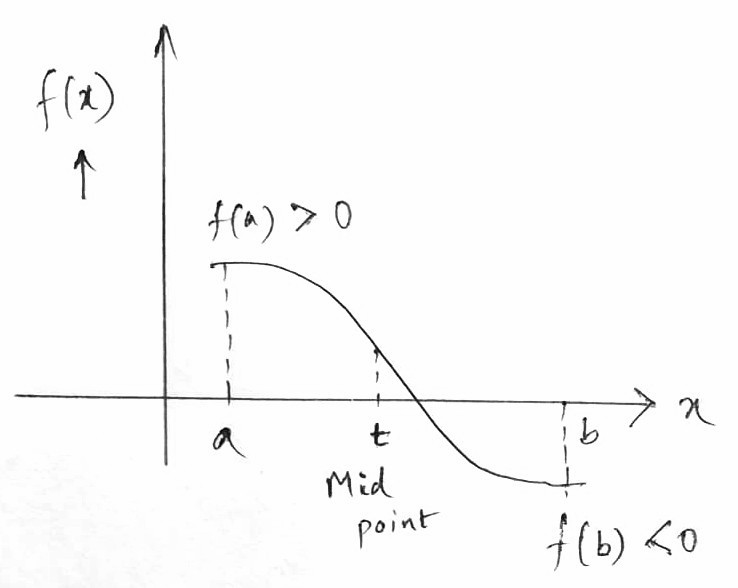
\includegraphics[scale=0.3]{code/sort/pic/bisection.jpeg}
	\caption{Bisection method}
\end{figure}

\begin{lstlisting}
'''Bisection method'''
def f(x):
    # The equation to be solved is written in form f(x) = 0
    return x**3-3*x**2-7

def bisection_method(tolerance):
    a = int(input('Type the value of initial guess a = '))
    b = int(input('Type the value of initial guess b = '))
    
    while f(a)*f(b) > 0:
        print('f(a) = ', f(a))
        print('f(b) = ', f(b))
        print('Solution cannot be found. Enter new values of a and b.')
        a = int(input('Type the value of initial guess a = '))
        b = int(input('Type the value of initial guess b = '))
    print('f(a) = ', f(a))
    print('f(b) = ', f(b))
    if f(a)*f(b) < 0:
        t = (a + b)/2
        error = abs(f(t))
        iteration_counter = 1
        print('Iteration ',iteration_counter,': Value = ',t, ': Error = ', error)
        while error > tolerance:
            iteration_counter += 1
            if f(a)*f(t)>0: 
                a = t
            else:
                b = t          
            t = (a + b)/2
            error = abs(f(t))
            print('Iteration ',iteration_counter,': Value = ',t, ': Error = ', error)
    return t


if __name__ == "__main__":
    tolerance = 0.0001
    bisection_method(tolerance)
\end{lstlisting}
\textbf{Output}
\begin{lstlisting}
Type the value of initial guess a = 2
Type the value of initial guess b = 6
f(a) =  -11
f(b) =  101
Iteration  1 : Value =  4.0 : Error =  9.0
Iteration  2 : Value =  3.0 : Error =  7.0
Iteration  3 : Value =  3.5 : Error =  0.875
Iteration  4 : Value =  3.75 : Error =  3.546875
Iteration  5 : Value =  3.625 : Error =  1.212890625
Iteration  6 : Value =  3.5625 : Error =  0.138916015625
Iteration  7 : Value =  3.53125 : Error =  0.375457763671875
Iteration  8 : Value =  3.546875 : Error =  0.12013626098632812
Iteration  9 : Value =  3.5546875 : Error =  0.008922100067138672
Iteration  10 : Value =  3.55078125 : Error =  0.05572384595870972
Iteration  11 : Value =  3.552734375 : Error =  0.02343008667230606
Iteration  12 : Value =  3.5537109375 : Error =  0.007261299528181553
Iteration  13 : Value =  3.55419921875 : Error =  0.0008285733638331294
Iteration  14 : Value =  3.553955078125 : Error =  0.0032168197649298236
Iteration  15 : Value =  3.5540771484375 : Error =  0.0011942373766942183
Iteration  16 : Value =  3.55413818359375 : Error =  0.00018286055114913324
Iteration  17 : Value =  3.554168701171875 : Error =  0.00032284927007708575
Iteration  18 : Value =  3.5541534423828125 : Error =  6.999257541195902e-05
\end{lstlisting}

\subsection{Secant method}
\begin{enumerate}
    \item Choose two initial guesses $x_0$ and $x_1$.
    \item For $n = 1,2,3, \cdots $
    $$x_{n+1} = x_n - \dfrac{x_n-x_{n-1}}{f(x_n)-f(x_{n-1})}f(x_n)$$
    \item Iteration stops for $n=k$ when $f(x_k) < \epsilon$ where $\epsilon$ is the specified tolerance and the solution is then given by the value of $x_k$.
\end{enumerate}
\noindent N.B. This method does not always converge.
\vspace{5mm}

\begin{figure}[ht]
	\centering
	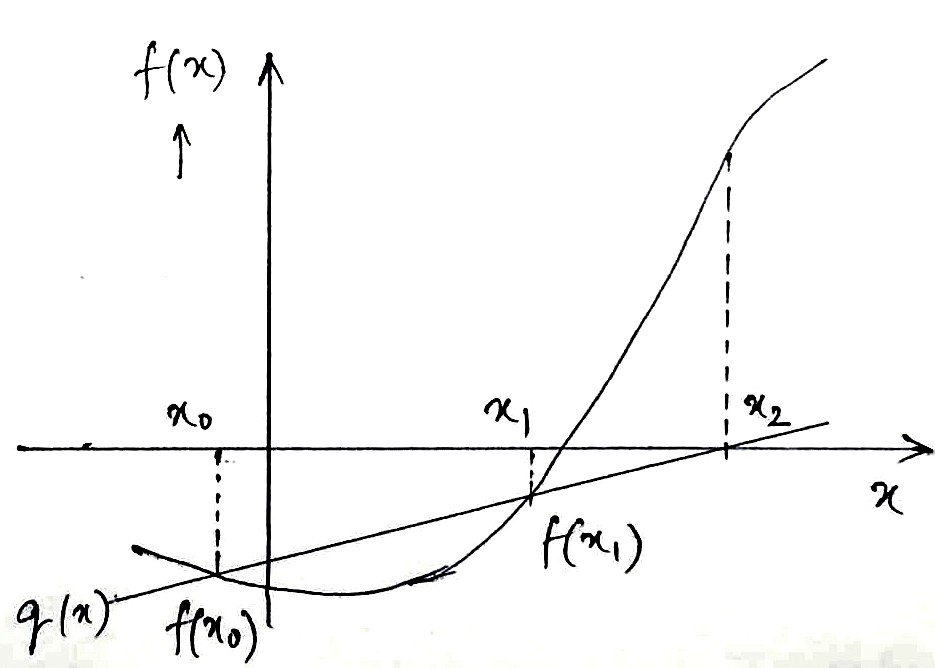
\includegraphics[scale=0.2]{code/sort/pic/secant.jpeg}
	\caption{Secant method: geometric interpretation}
\end{figure}
\noindent \textbf{Geometric interpretation}: Let $x_0$ and $x_1$ be the initial approximations for the root $s$ of $f(x)=0$. $f(x_0)$ and $f(x_1)$ are their function values. Let $x_2$ be the point of intersection of the line joining $\left(x_0, f(x_0)\right)$ and $\left(x_1, f(x_1)\right)$.
$$\dfrac{f(x_1)-f(x_0)}{x_1-x_0} = \dfrac{0-f(x_1)}{x_2-x_1}$$
\noindent since $f(x_2)=0$.
$$\Rightarrow x_2 = x_1 - \dfrac{x_1-x_0}{f(x_1)-f(x_0)}f(x_1)$$
\noindent General rule:
$$x_{n+1} = x_n - \dfrac{x_n-x_{n-1}}{f(x_n)-f(x_{n-1})}f(x_n)$$

\begin{lstlisting}
'''Secant method'''
import sys

def f(x):
    # The equation to be solved is written in form f(x) = 0
    return x**3-3*x**2-7

def secant_method(tolerance):
    x0 = int(input('Type the value of the first initial guess x0 = '))
    x1 = int(input('Type the value of the second initial guess x1 = '))
    iteration_counter = 0
    while abs(f(x1)) > tolerance and iteration_counter < 100:
        try:
            denominator = float(f(x1) - f(x0))/(x1 - x0)
            x = x1 - float(f(x1))/denominator
        except ZeroDivisionError:
            print("Error! - denominator zero for x = ", x)
            sys.exit(1)     # Abort with error
        x0 = x1
        x1 = x
        iteration_counter += 1
        error = abs(f(x1))
        print('Iteration ', iteration_counter,': Value = ',x1, ': Error = ', error)
    return x1


if __name__ == "__main__":
    tolerance = 0.0001
    secant_method(tolerance)
\end{lstlisting}
\textbf{Output}
\begin{lstlisting}
Type the value of the first initial guess x0 = 1
Type the value of the second initial guess x1 = 4
Iteration  1 : Value =  2.5 : Error =  10.125
Iteration  2 : Value =  3.2941176470588234 : Error =  3.808467331569311
Iteration  3 : Value =  3.7729200652528556 : Error =  4.0024597927268815
Iteration  4 : Value =  3.527573079295066 : Error =  0.435000977724485
Iteration  5 : Value =  3.5516242617830494 : Error =  0.04179231189964128
Iteration  6 : Value =  3.554180549595233 : Error =  0.0005191945178779633
Iteration  7 : Value =  3.5541491819902817 : Error =  6.06673715708439e-07
\end{lstlisting}

\subsection{Newton-Raphson method}
\begin{enumerate}
    \item Choose an initial guess $x_0$.
    \item For $n = 0,1,2, \cdots $
    $$x_{n+1} = x_n - \dfrac{f(x_n)}{f'(x_n)}$$
    provided $f'(x)$, the derivative of $f(x)$, exists at $x=x_n$.
    \item Iteration stops for $n=k$ when $f(x_k) < \epsilon$ where $\epsilon$ is the specified tolerance and the solution is then given by the value of $x_k$.
\end{enumerate}
\noindent N.B. This method does not always converge.
\vspace{5mm}

\begin{figure}[ht]
	\centering
	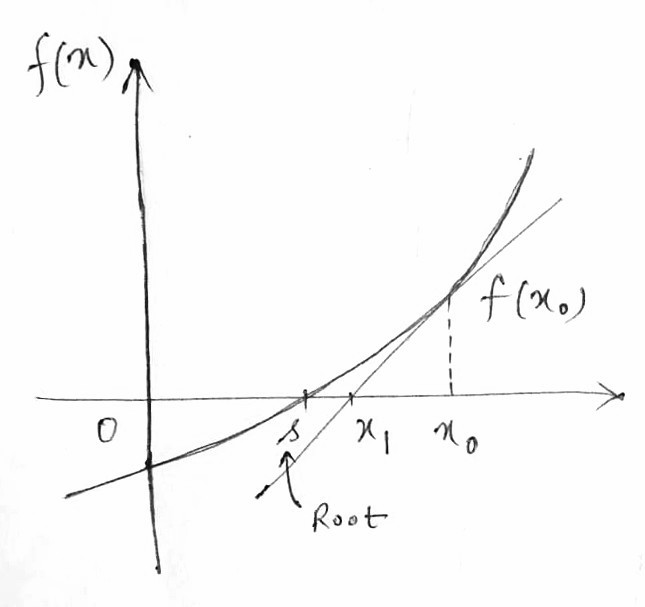
\includegraphics[scale=0.3]{code/sort/pic/newtonraphson.jpeg}
	\caption{Newton-Raphson method: geometric interpretation}
\end{figure}

\noindent \textbf{Geometric interpretation}: Let $x_0$ be the initial guess for the root $s$ of $f(x)=0$. The tangent line to $y=f(x)$ at point $(x_0, f(x_0)$ has the following equation:
$$f'(x_0) = \dfrac{y-f(x_0)}{x-x_0}$$
\noindent If $x_1$ is the $x$-intercept of the tangent lin, then
\begin{align*}
    f'(x_0) &= -\dfrac{f(x_0)}{x_1-x_0}\\
    x_1 &= x_0 - \dfrac{f(x_0)}{x_1-x_0}
\end{align*}
\noindent $x_1$ is the new Newton-Raphson estimate of the root. Next tangent line at $\left(x_1, f(x_1)\right)$ will cut the $x$-axis much closer to the root.
$$\Rightarrow x_2 = x_1 - \dfrac{x_1-x_0}{f(x_1)-f(x_0)}f(x_1)$$
\noindent General rule:
$$x_{n+1} = x_n - \dfrac{x_n-x_{n-1}}{f(x_n)-f(x_{n-1})}f(x_n)$$

\begin{lstlisting}
'''Newton-Raphson method'''
def f(x):
# The equation to be solved is written in form f(x) = 0
    return x**3-3*x**2-7

def df_dx(x):
    # The derivative of f(x) w.r.t x
    return 3*x**2-6*x

def newton_raphson(tolerance):
    x0 = int(input('Type the value of the first initial guess x0 = '))
    iteration_counter = 0
    error = abs(f(x0))
    if error <= tolerance:
        return x0
    while error >= tolerance and iteration_counter <= 100:
        x1 = x0 - (f(x0)/df_dx(x0))
        x0 = x1
        error = abs(f(x0))
        iteration_counter += 1
        print('Iteration ', iteration_counter,': Value = ', x1, ': Error = ', error)
    return x1


if __name__ == "__main__":
    tolerance = 0.0001
    newton_raphson(tolerance)
\end{lstlisting}
\textbf{Output}
\begin{lstlisting}
Type the value of the first initial guess x0 = 3
Iteration  1 : Value =  3.7777777777777777 : Error =  4.100137174211248
Iteration  2 : Value =  3.574278322440087 : Error =  0.3366729108147055
Iteration  3 : Value =  3.5543341033367417 : Error =  0.003063993300784773
Iteration  4 : Value =  3.5541492344047616 : Error =  2.618884451521808e-07
\end{lstlisting}

\subsection{Regula-falsi method}
\begin{enumerate}
    \item Choose two values $a$ and $b$ such that $a<b$ and $f(a)f(b) < 0$.
    \item Find the midpoint $t = \dfrac{af(b)-bf(a)}{f(b)-f(a)}$.
    \item If $f(t) = 0$, then $t$ is a solution.
    \item If $f(t) \neq 0$, then
    \begin{enumerate}
        \item If $f(a)$ and $f(t)$ are of same sign, replace $a \leftarrow t$.
        \item Else, replace $b \leftarrow t$.
    \end{enumerate}
    \item Go back to step 2.
    \item Iteration stops when $f(t) < \epsilon$ where $\epsilon$ is the specified tolerance and the solution is then given by the value of $t$.
\end{enumerate}

\vspace{5mm}

\begin{figure}[ht]
	\centering
	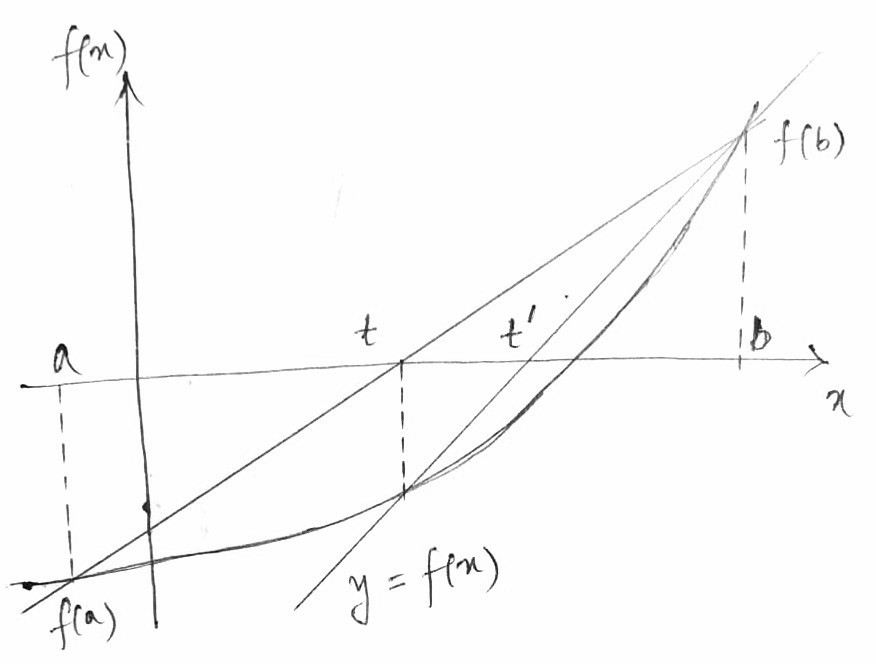
\includegraphics[scale=0.26]{code/sort/pic/regulafalsi.jpeg}
	\caption{Regula-falsi method: geometric interpretation}
\end{figure}

\noindent \textbf{Geometric interpretation}: The equation of a straight line passing through the points $(a, f(a))$ and $(b, f(b))$ is
$$\dfrac{y-f(a)}{x-a} = \dfrac{f(b)-f(a)}{b-a}$$
\noindent At the intersection point with $x$-axis,
\begin{align*}
    \dfrac{-f(a)}{x-a} &= \dfrac{f(b)-f(a)}{b-a}\\
    \Rightarrow t\left(f(b)-f(a)\right) &= af(b)-af(a)-bf(a)+af(a)\\
    \Rightarrow t &= \dfrac{af(b)-bf(a)}{f(b)-f(a)}
\end{align*}
\noindent Now if $f(t)f(a) > 0$, $a$ is replaced by $t$.
\begin{lstlisting}
'''Regula-falsi method'''
def f(x):
    # The equation to be solved is written in form f(x) = 0
    return x**3-3*x**2-7

def regulafalsi_method(tolerance):
    a = int(input('Type the value of initial guess a = '))
    b = int(input('Type the value of initial guess b = '))
    
    while f(a)*f(b) > 0:
        print('f(a) = ', f(a))
        print('f(b) = ', f(b))
        print('Solution cannot be found. Enter new values of a and b.')
        a = int(input('Type the value of initial guess a = '))
        b = int(input('Type the value of initial guess b = '))
    print('f(a) = ', f(a))
    print('f(b) = ', f(b))
    if f(a)*f(b) < 0:
        t = (a*f(b) - b*f(a))/(f(b) - f(a))
        error = abs(f(t))
        iteration_counter = 1
        print('Iteration ',iteration_counter,': Value = ',t, ': Error = ', error)
        while error > tolerance:
            iteration_counter += 1
            if f(a)*f(t)>0: 
                a = t
            else:
                b = t          
            t = (a*f(b) - b*f(a))/(f(b) - f(a))
            error = abs(f(t))
            print('Iteration ',iteration_counter,': Value = ',t, ': Error = ', error)
    return t


if __name__ == "__main__":
    tolerance = 0.0001
    regulafalsi_method(tolerance)
\end{lstlisting}
\textbf{Output}
\begin{lstlisting}
Type the value of initial guess a = 1
Type the value of initial guess b = 4
f(a) =  -9
f(b) =  9
Iteration  1 : Value =  2.5 : Error =  10.125
Iteration  2 : Value =  3.2941176470588234 : Error =  3.808467331569311
Iteration  3 : Value =  3.504004576659039 : Error =  0.8118075786435668
Iteration  4 : Value =  3.5450421571877415 : Error =  0.1502786735172137
Iteration  5 : Value =  3.5525141111646144 : Error =  0.02707494028368984
Iteration  6 : Value =  3.553856257297017 : Error =  0.0048540143135582525
Iteration  7 : Value =  3.5540967484931585 : Error =  0.0008694628781782399
Iteration  8 : Value =  3.5541398217013684 : Error =  0.00015571566942895743
Iteration  9 : Value =  3.5541475357252508 : Error =  2.7886966961432336e-05
\end{lstlisting}

\end{document}
